\documentclass[12pt,a4paper]{article}
\usepackage{graphicx}
\usepackage{geometry}
\usepackage{booktabs}
\usepackage{threeparttable} % Add to preamble
\usepackage{cite}
\usepackage{amsmath,amssymb}
\usepackage{hyperref}
\usepackage{multirow}
\usepackage{array}
\usepackage{xcolor}
\usepackage{colortbl}
\usepackage{longtable}
\usepackage{pdflscape}
\usepackage{caption}
\usepackage{subcaption}
\usepackage{float}
\usepackage{xurl}
\usepackage{enumitem}
% \usepackage{microtype}

% Start sections on new pages
\usepackage{titlesec}
\newcommand{\sectionbreak}{\clearpage}

% Number figures and tables by section
\usepackage{chngcntr}
\counterwithin{figure}{section}
\counterwithin{table}{section}

% Center Table of Contents, List of Figures, and List of Tables titles
\makeatletter
\renewcommand\tableofcontents{%
    \section*{\centering\contentsname}%
    \@starttoc{toc}%
}
\renewcommand\listoffigures{%
    \section*{\centering\listfigurename}%
    \@starttoc{lof}%
}
\renewcommand\listoftables{%
    \section*{\centering\listtablename}%
    \@starttoc{lot}%
}
\makeatother

\geometry{a4paper, margin=1in}
\captionsetup{font=small, labelfont=bf, skip=6pt}
\usepackage{iftex}
\ifXeTeX
  \usepackage{fontspec}
  \newfontfamily\banglafont[Script=Bengali]{Kalpurush}
\else
  \providecommand{\banglafont}{}
\fi
\ifdefined\DeclareUnicodeCharacter
  \DeclareUnicodeCharacter{0964}{\textbar}
\fi

\begin{document}

\begin{titlepage}
\centering

\vspace*{0.5cm}

{\large \textbf{Comparative Analysis of Locally Produced Bitumen and Imported Low-Cost Bitumen for Bangladesh Road Construction (Focusing on Aggregate Shape)}\par}

\vspace{0.5cm}

by

\vspace{0.5cm}

Md. Rakibul Hasan Mridha\\
ID: 2020333545

\vspace{0.2cm}

Md Sagor Hossain Saddas\\
ID: 2020333553

\vspace{0.5cm}

Course Code: CE 800

\vspace{0.5cm}

Bachelor of Science in Civil Engineering

\vspace{0.2cm}

IN

\vspace{0.2cm}

DEPARTMENT OF CIVIL ENGINEERING

\vspace{0.5cm}

\textbf{Supervised by}

\vspace{0.1cm}

Md Johir Bin Alam\\
Professor\\
Department of CEE\\
Shahjalal University of Science \& Technology

\vspace{0.4cm}

\textbf{Co-Supervised by}

\vspace{0.1cm}

Mohiuddin Arif\\
Lecturer\\
Department of Civil Engineering\\
Sylhet Engineering College

\vspace{0.5cm}


\includegraphics[width=0.25\textwidth]{graphics/sec logo.png}

\vspace{0.3cm}

Sylhet Engineering College\\
(Shahjalal University of Science \& Technology)

\vspace{0.2cm}

Sylhet-3100, Bangladesh

\vspace{0.3cm}

August 2026

\end{titlepage}

\newpage
\pagenumbering{roman}
\phantomsection
\addcontentsline{toc}{section}{Candidate's Declaration}

\begin{center}
    \Large \textbf{Candidate's Declaration}
\end{center}

\vspace{1.5cm}

\noindent This is to certify that the work presented in this thesis entitled, \textbf{``Comparative Analysis of Locally Produced Bitumen and Imported Low-Cost Bitumen for Bangladesh Road Construction (Focusing on Aggregate Shape)''}, is the outcome of the research carried out by the authors under the supervision of \textbf{Md Johir Bin Alam, Professor, Department of CEE, Shahjalal University of Science \& Technology, Bangladesh}, and the co-supervision of \textbf{Mohiuddin Arif, Lecturer, Department of Civil Engineering, Sylhet Engineering College, Bangladesh}.

\vspace{0.5cm}

\noindent It is also declared that neither this thesis nor any part thereof has been submitted anywhere else for the award of any degree, diploma, or other qualifications.

\vspace{2cm}

\noindent \textbf{Signature of the Candidates}

\vspace{2cm}

% First row of candidate signatures
\noindent
\begin{minipage}[t]{0.45\textwidth}
    \rule{0.8\textwidth}{0.5pt}\\
    Md. Rakibul Hasan Mridha\\
    Reg. No.: 2020333545
\end{minipage}
\hfill
\begin{minipage}[t]{0.45\textwidth}
    \rule{0.8\textwidth}{0.5pt}\\
    Md Sagor Hossain Saddas\\
    Reg. No.: 2020333553
\end{minipage}

\newpage
\phantomsection
\addcontentsline{toc}{section}{Recommendation Letter from Thesis Supervisor}
\begin{center}
    \Large \textbf{Recommendation Letter from Thesis Supervisor}
\end{center}
\vspace{1.5cm}



The thesis entitled \textbf{``Comparative Analysis of Locally Produced Bitumen and Imported Low-Cost Bitumen for Bangladesh Road Construction (Focusing on Aggregate Shape)''} submitted by the students:
\begin{enumerate}
    \item Md. Rakibul Hasan Mridha (Reg. No.: 2020333545)
    \item Md Sagor Hossain Saddas (Reg. No.: 2020333553)
\end{enumerate}
is a record of research work carried out under our supervision and we, hereby, approve that the report is submitted in partial fulfilment of the requirement for the award of their Bachelor's Degree.

\vspace{3.5cm}

\noindent
\begin{minipage}[t]{0.48\textwidth}
    \noindent\makebox[2.5in]{\hrulefill} \\
    Signature of the Supervisor \\
    \textbf{Md Johir Bin Alam} \\
    Professor \\
    Department of CEE \\
    Shahjalal University of Science \& Technology
\end{minipage}
\hfill
\begin{minipage}[t]{0.48\textwidth}
    \noindent\makebox[2.5in]{\hrulefill} \\
    Signature of the Co-Supervisor \\
    \textbf{Mohiuddin Arif} \\
    Lecturer \\
    Department of Civil Engineering \\
    Sylhet Engineering College
\end{minipage}

\vspace{2cm}

\noindent \textbf{Date:} \makebox[2.5in]{\hrulefill}

\newpage
\phantomsection
\addcontentsline{toc}{section}{Certificate of Acceptance}
\begin{center}
    \Large \textbf{Certificate of Acceptance}
\end{center}
\vspace{1cm}

The thesis titled \textbf{``Comparative Analysis of Locally Produced Bitumen and Imported Low-Cost Bitumen for Bangladesh Road Construction (Focusing on Aggregate Shape)''} submitted by Md. Rakibul Hasan Mridha and Md Sagor Hossain Saddas; Student ID: 2020333545 and 2020333553, to the Department of Civil Engineering, Sylhet Engineering College, has been accepted as satisfactory in partial fulfillment of the requirement for the Degree of Bachelor of Science in Civil Engineering and approved as to its style and contents.

\vspace{0.8cm}

\begin{center}
    \textbf{BOARD OF EXAMINERS}
\end{center}

\vspace{0.8cm}

\noindent
\begin{minipage}[t]{0.70\textwidth}
    \noindent\makebox[2.5in]{\hrulefill} \\
    Sibbir Ahmed \\
    Assistant Professor and Head of the Department \\
    Department of Civil Engineering \\
    Sylhet Engineering College
\end{minipage}
\hfill
\begin{minipage}[t]{0.28\textwidth}
    \raggedleft
    Chairperson
\end{minipage}

\vspace{0.8cm}

\noindent
\begin{minipage}[t]{0.70\textwidth}
    \noindent\makebox[2.5in]{\hrulefill} \\
    Tahia Rabbi \\
    Assistant Professor \\
    Department of Civil Engineering \\
    Sylhet Engineering College
\end{minipage}
\hfill
\begin{minipage}[t]{0.28\textwidth}
    \raggedleft
    Internal Examiner
\end{minipage}

\vspace{0.8cm}

\noindent
\begin{minipage}[t]{0.70\textwidth}
    \noindent\makebox[2.5in]{\hrulefill} \\
    Mohiuddin Arif \\
    Lecturer \\
    Department of Civil Engineering \\
    Sylhet Engineering College
\end{minipage}
\hfill
\begin{minipage}[t]{0.28\textwidth}
    \raggedleft
    Internal Examiner
\end{minipage}

\vspace{0.8cm}

\noindent
\begin{minipage}[t]{0.70\textwidth}
    \noindent\makebox[2.5in]{\hrulefill} \\
    Md. Titumir Hassan \\
    Workshop Maintenance Engineer \\
    Department of Civil Engineering \\
    Sylhet Engineering College
\end{minipage}
\hfill
\begin{minipage}[t]{0.28\textwidth}
    \raggedleft
    Internal Examiner
\end{minipage}

\vspace{0.8cm}

\noindent
\begin{minipage}[t]{0.70\textwidth}
    \noindent\makebox[2.5in]{\hrulefill} \\
    Md Johir Bin Alam \\
    Professor \\
    Department of CEE \\
    Shahjalal University of Science \& Technology
\end{minipage}
\hfill
\begin{minipage}[t]{0.28\textwidth}
    \raggedleft
    External Examiner
\end{minipage}

\newpage
\phantomsection
\addcontentsline{toc}{section}{Acknowledgement}
\begin{center}
    \Large \textbf{Acknowledgement}
\end{center}
\vspace{1cm}

We would like to thank the Department of Civil Engineering, Sylhet Engineering College, Sylhet for supporting this research.

We are very thankful to our honorable supervisor Md Johir Bin Alam and co-supervisor Mohiuddin Arif for their worthy support and directions.

We are also very grateful to the authors and researchers for their previous works which played a very important role in our thesis.

Finally, we must acknowledge with due respect the constant support and patience of our parents.

\vspace{2cm}

\begin{flushright}
\textbf{The Authors}\\
\end{flushright}

\newpage
\phantomsection
\addcontentsline{toc}{section}{Abstract}
\begin{abstract}
\noindent Flexible pavements in Bangladesh frequently experience premature distress due to inconsistent imported bitumen and suboptimal aggregate morphology. This study investigates the combined effect of bitumen source quality and aggregate particle shape on the Marshall mix properties of bituminous mixtures. A laboratory-based comparative analysis evaluated four mix combinations: locally produced bitumen and imported bitumen, each paired with either natural aggregates or a 20\% cubical aggregate replacement. Specimens were compacted at 75 blows per face to simulate heavy traffic conditions according to Roads and Highways Department specifications, with an established optimum binder content of 5.0\%. Results indicated that combining local bitumen with 20\% cubical aggregates improved both volumetric and mechanical characteristics. This mix achieved a peak Marshall stability of 13.3\,kN (2991\,lbs) and maintained an air void content of 5.20\%. This represents a 167\% improvement in stability and a 50\% reduction in permanent deformation compared to the imported bitumen control mix, which exhibited the lowest stability and highest flow. In contrast, combining imported bitumen with cubical aggregates reduced air voids to 2.59\%, increasing the risk of pavement bleeding. The data indicates that utilizing local bitumen with shape-optimized aggregates increases the load-bearing capacity and rutting resistance of flexible pavements, offering an evidence-based material selection strategy for road construction in subtropical climates.

\vspace{0.5cm}

\noindent \textbf{Keywords:} bitumen, aggregate shape, Marshall stability, cubical aggregate, Bangladesh, road construction, flexible pavement
\end{abstract}

\newpage
\tableofcontents
\newpage
\phantomsection
\addcontentsline{toc}{section}{\listfigurename}
\listoffigures
\newpage
\phantomsection
\addcontentsline{toc}{section}{\listtablename}
\listoftables
\clearpage

\clearpage
\pagenumbering{arabic}
\setcounter{page}{1}
\section{Introduction}

\subsection{Background}

Bangladesh has an extensive road network spanning approximately 375,000\,km, of which more than 90\% comprises flexible pavements constructed using bituminous materials. The performance of these pavements depends on the quality of the constituent materials, specifically the bituminous binder and the mineral aggregates~\cite{werkineh2020assessment}. Bitumen provides the adhesive and cohesive properties necessary to bind aggregate particles into a durable pavement matrix. In Bangladesh, Eastern Refinery Limited in Chittagong is the sole domestic producer of bitumen, supplying penetration-grade 60/70 bitumen at a controlled price of approximately Tk\,6,300 per unit. Because domestic supply often falls short of national demand, contractors frequently source imported bitumen from international markets.

The Roads and Highways Department (RHD) has periodically imposed restrictions on certain imported bitumen grades due to concerns regarding their quality and the resulting pavement deterioration~\cite{imran2025developing}. Nevertheless, imported low-cost bitumen continues to be used in numerous road construction projects across the country for short-term economic reasons.

The aggregate component of hot mix asphalt (HMA) constitutes approximately 92\% to 96\% of the total mixture by weight and influences the structural performance of the pavement~\cite{rajkumar2018experimental}. Among aggregate properties, particle shape affects the interlocking behaviour, compaction characteristics, and resistance to permanent deformation of bituminous mixes~\cite{teja2020effect}. Cubical aggregates, characterised by roughly equal dimensions along all three axes, exhibit stronger mechanical interlock and internal friction compared to flaky, elongated, or blade-shaped particles~\cite{sumanth2017study}. While the effect of aggregate shape is documented, its combined effect with local versus imported bitumen source quality has not been extensively studied in the context of Bangladesh.

\subsection{Problem Statement}

The quality disparity between locally refined bitumen from Eastern Refinery and imported alternatives affects Bangladesh's road infrastructure. Imported bitumen often exhibits variable penetration grades and rheological properties, which have been associated with accelerated pavement distress, including rutting, stripping under monsoon conditions, and fatigue cracking~\cite{khairandish2020influence}. These distress modes reduce structural integrity and increase maintenance frequency, affecting the pavement service life.

Existing research addresses bitumen characterisation and aggregate shape effects independently; however, few studies have integrated these variables within an experimental framework tailored to the climatic and traffic conditions in Bangladesh~\cite{sood2015evaluation}. The subtropical monsoon climate, which includes summer temperatures exceeding 40$^{\circ}$C and prolonged heavy rainfall, subjects bituminous pavements to thermal and moisture-induced stresses. A gap remains in understanding how bitumen source quality and aggregate particle shape combined affect the Marshall mix design properties of flexible pavements in this region.

\subsection{Objectives of the Study}

The primary objective of this study is to assess and compare the performance of locally produced bitumen from Eastern Refinery with imported low-cost bitumen for road construction applications in Bangladesh, with particular emphasis on the role of aggregate particle shape. The specific objectives are as follows:

\begin{enumerate}[label=\roman*.]
    \item To compare the physical properties (penetration, softening point, ductility, specific gravity, and flash point and fire point) of local and imported 60/70 penetration-grade bitumen.
    \item To determine the optimum binder content (OBC) using the Marshall method for the control mix with local bitumen.
    \item To evaluate the effect of cubical aggregate shape (20\% replacement of coarse fraction) on the Marshall mix design properties of bituminous mixes.
    \item To assess the performance of the four mix combinations in terms of Marshall stability, flow, and volumetric properties.
    \item To compare the four bituminous mixes in terms of required pavement thickness, cost effectiveness, and load bearing capacity.
    \item To provide evidence-based recommendations for material selection in Bangladesh's road construction practice.
\end{enumerate}

\subsection{Scope and Limitations}

This study is limited to a laboratory-scale investigation employing the Marshall mix design method. The experimental programme utilises 60/70 penetration-grade bitumen from two sources (local Eastern Refinery and imported) and crushed stone aggregates conforming to MoRTH Grading-II for Dense Bituminous Macadam (DBM) with a nominal maximum aggregate size (NMAS) of 19\,mm. Four mix combinations are investigated, incorporating natural (as-received) and shape-sorted (20\% cubical replacement) aggregates.

The following limitations are acknowledged:
\begin{itemize}
    \item \textbf{Aggregate Morphological Evaluation:} The shape classification of coarse aggregates was solely based on the Zingg diagram, utilizing elongation and flatness ratios. The relevant shape parameters are defined as follows:
    \begin{align*}
        \text{Elongation ratio} &= d_i / d_l \\
        \text{Flatness ratio} &= d_s / d_i \\
        \text{Shape factor} &= \frac{d_s}{\sqrt{d_i \cdot d_l}} \\
        \text{Sphericity} &= \sqrt[3]{\frac{d_s \cdot d_i}{d_l^2}}
    \end{align*}
    where $d_l$, $d_i$, and $d_s$ represent the longest, intermediate, and shortest dimensions of the aggregate, respectively. With these ratios, the aggregates are classified into Blade shape, Disc shape, Cubical shape, and Rod shape, as shown in Table~\ref{tab:shape_classification_limitations}.
    
    \begin{table}[H]
        \centering
        \caption{Aggregate shape classification using Zingg's classification}
        \label{tab:shape_classification_limitations}
        \begin{tabular}{@{}lcc@{}}
            \toprule
            \textbf{Aggregate shape} & \textbf{Elongation ratio} & \textbf{Flatness ratio} \\
            \midrule
            Blade & $< 2/3$ & $< 2/3$ \\
            Rod & $< 2/3$ & $> 2/3$ \\
            Disc & $> 2/3$ & $< 2/3$ \\
            Cubical & $> 2/3$ & $> 2/3$ \\
            \bottomrule
        \end{tabular}
    \end{table}

    A more comprehensive metric incorporating the aforementioned Shape factor or Sphericity, or the Particle Index (PI), was not determined. Evaluating the Particle Index (PI) would have provided a more adequate measure of the combined contributions of particle shape, angularity, and surface texture to the dense packing configuration and internal resistance of the mix.
    \item \textbf{Material Sourcing:} Aggregates were sourced from a single quarry in the Sylhet region; therefore, the results may vary with aggregates of different geological origins or mineralogical compositions.
    \item \textbf{Binder Modification:} The scope of this investigation was restricted to unmodified penetration-grade binders. The performance enhancement using polymer-modified binders (e.g., adding 5\% SBS polymer) was not included.
    \item \textbf{Gradation Scope:} The study is strictly confined to the 19\,mm NMAS DBM gradation and does not extend to other critical pavement layers such as Bituminous Concrete (BC) or Stone Matrix Asphalt (SMA).
\end{itemize}

\subsection{Thesis Organisation}

The remainder of this thesis is organised as follows. Section~2 presents a review of the existing literature on bitumen characterisation, aggregate shape effects, and Marshall mix design. Section~3 details the experimental methodology, including materials, specimen preparation, and the testing programme. Section~4 presents the experimental results and discusses the findings in the context of prior research. Section~5 summarises the conclusions drawn from this study and provides recommendations for future work.



\section{Literature Review}

\subsection{Bitumen Grading and Pavement Performance in Tropical Climates}
The performance of flexible pavements depends on the structural capacity of the underlying materials, particularly in tropical and subtropical regions that experience high traffic volumes and climatic variations. Imran et al.~\cite{imran2025developing} developed a pavement quality index, noting that traffic growth and temperature fluctuations accelerate pavement deterioration. Their study observed that inadequate quality control during construction leads to distresses such as rutting and thermal cracking. Similarly, Werkineh and Demissie~\cite{werkineh2020assessment} investigated pavement failures along the Assosa-Mendi road network, reporting that weak sub-surface materials correlate with alligator cracking and pothole formation. These studies indicate that high-quality, temperature-resistant bituminous binders and sound granular bases are required to maintain highway infrastructure in these environments.

\subsection{Aggregate Shape and Its Influence on Mix Design}
The morphological characteristics of coarse aggregates---specifically their shape, angularity, and texture---affect the mechanical stability and volumetric properties of hot mix asphalt (HMA). Khairandish and Chopra~\cite{khairandish2020influence} indicated that flat and elongated particles tend to fracture under traffic loads, reducing the shear resistance and increasing the rutting susceptibility of bituminous mixes. Teja and Krishna~\cite{teja2020effect} investigated dense bituminous macadam (DBM) mixes containing various proportions of differently shaped aggregates. Their study observed that replacing conventional aggregates with 20\% cubical particles increased Marshall stability due to aggregate interlock and internal friction, whereas blade-shaped aggregates reduced mix workability and strength. Rajkumar et al.~\cite{rajkumar2018experimental} reported that a higher percentage of flaky and elongated aggregates increases air voids, which can affect the fatigue life of the pavement. Sumanth et al.~\cite{sumanth2017study} showed that DBM mixes with cubical aggregates exhibited higher rutting resistance compared to other shapes.

In the context of South Asia, Verma and Khare~\cite{verma2024study} investigated the physical properties of crushed rock aggregates used in Indian road construction. They noted that aggregate characteristics influence the strength and serviceability of bituminous mixtures. Following the MORT\&H specifications, their study showed that Marshall parameters (Stability, Flow, VMA, VFB, and Air Voids) vary with aggregate particle shapes classified as cubical, rounded, and blade. They concluded that flakiness negatively affects the quality of the bituminous mix, supporting the use of cubical aggregates for pavement performance.

\subsection{Subgrade Stabilization and Economic Road Construction}
Strengthening the pavement foundation is a strategy for achieving cost-effective road construction. Sood and Bansal~\cite{sood2015evaluation} evaluated the use of industrial by-products, such as lime and fly ash, for subgrade soil stabilization. Their research observed that treating weak subgrade soils with these additives increases the California Bearing Ratio (CBR) up to an optimal limit. A stabilized subgrade reduces the required thickness of the overlying flexible pavement layers, lowering the volume of construction materials required for highway projects.

\subsection{Influence of Bitumen Properties on Stripping and Durability}
The durability of bitumen during its design life is a primary concern in pavement engineering. Bagampadde et al.~\cite{bagampadde2006impact} examined the effect of aggregate and bitumen mixtures on stripping. They reported that compositions with lower penetration grade asphalt showed higher durability due to greater resilient and tensile strength. However, bitumen characteristics such as acid number, penetration grade, and molecular size distribution had a minimal effect on moisture sensitivity.

\subsection{Research Gap}
While prior investigations have documented the independent effects of cubical aggregates~\cite{teja2020effect, sumanth2017study} and subgrade stabilization~\cite{sood2015evaluation}, the combined influence of aggregate morphology and varying qualities of bituminous binders remains unexplored in the context of Bangladesh. Specifically, the interaction between a 20\% cubical aggregate replacement and penetration-grade 60/70 bitumen sourced locally compared to imported variants requires systematic evaluation. This study addresses this gap by comparing these mix variants to inform material selection in the region.

Additionally, Bagampadde et al.~\cite{bagampadde2006impact} reported that the inherent characteristics of bitumen have a minimal influence on the moisture sensitivity of bituminous mixtures. Because all experimental mixes in this study utilized aggregates sourced from a single quarry in Sylhet, additional moisture damage assessments were not conducted. The investigation instead focused on evaluating the load-bearing capacity of the two bitumen types using Marshall stability testing.

\section{Methodology}

\subsection{General}

This section describes the materials, experimental procedures, and testing programme. The investigation includes material characterisation, aggregate gradation and shape classification, mix design, specimen preparation, and performance evaluation. The overall experimental methodology is illustrated in Figure~\ref{fig:flowchart}.

\begin{figure}[htbp]
    \centering
    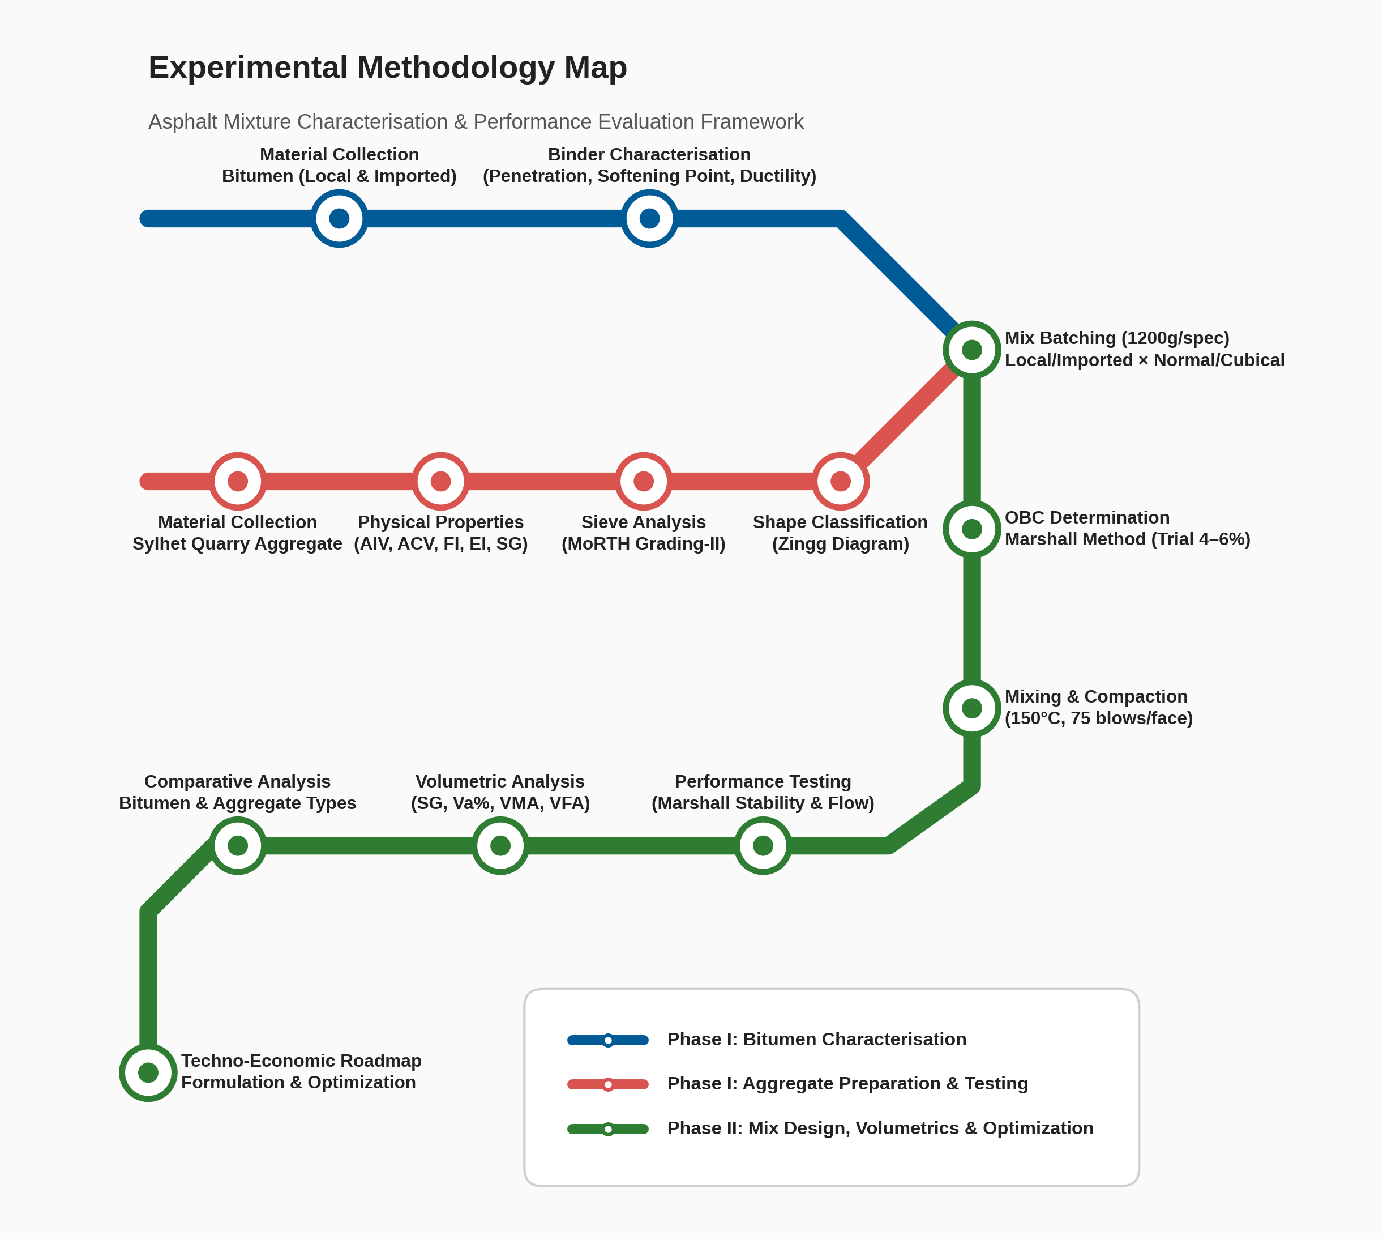
\includegraphics[width=0.85\textwidth]{graphics/methodology_flowchart.pdf}
    \caption{Flowchart of the experimental methodology adopted in this study.}
    \label{fig:flowchart}
\end{figure}

\subsection{Materials}

\subsubsection{Bitumen}

Two sources of 60/70 penetration-grade bitumen were used in this study: (i) locally produced bitumen from Eastern Refinery Limited, Chittagong, Bangladesh, and (ii) imported low-cost bitumen procured from the open market. Both binders were subjected to standard characterisation tests in accordance with the relevant ASTM standards. The tests included penetration at 25$^{\circ}$C (ASTM D5~--- Standard Test Method for Penetration of Bituminous Materials), softening point by the ring-and-ball method (ASTM D36~--- Standard Test Method for Softening Point of Bitumen), ductility at 25$^{\circ}$C (ASTM D113~--- Standard Test Method for Ductility of Asphalt Materials), kinematic viscosity (ASTM D2170~--- Standard Test Method for Kinematic Viscosity of Asphalts), specific gravity at 25$^{\circ}$C (ASTM D70~--- Standard Test Method for Density of Semi-Solid Asphalt Binder), and flash point by the Cleveland open cup method (ASTM D92~--- Standard Test Method for Flash and Fire Points). The physical properties of the local and imported bitumen are presented in Table~\ref{tab:local_bitumen} and Table~\ref{tab:imported_bitumen}, respectively.

\begin{table}[htbp]
    \centering
    \caption{Physical properties of local bitumen (Eastern Refinery, 60/70 grade).}
    \label{tab:local_bitumen}
    \begin{tabular}{@{}llc@{}}
        \toprule
        \textbf{Property} & \textbf{Test Standard} & \textbf{Specification} \\
        \midrule
        Penetration at 25$^{\circ}$C (dmm) & ASTM D5 & 60--70 \\
        Softening Point ($^{\circ}$C) & ASTM D36 & 49--56 \\
        Ductility at 25$^{\circ}$C (cm) & ASTM D113 & $\geq$75 \\
        Kinematic Viscosity at 135$^{\circ}$C (cSt) & ASTM D2170 & $\geq$300 \\
        Specific Gravity at 25$^{\circ}$C & ASTM D70 & 0.97--1.02 \\
        Flash Point ($^{\circ}$C) & ASTM D92 & $\geq$230 \\
        \bottomrule
    \end{tabular}
\end{table}

\begin{table}[htbp]
    \centering
    \caption{Physical properties of imported low-cost bitumen (60/70 grade).}
    \label{tab:imported_bitumen}
    \begin{tabular}{@{}llc@{}}
        \toprule
        \textbf{Property} & \textbf{Test Standard} & \textbf{Specification} \\
        \midrule
        Penetration at 25$^{\circ}$C (dmm) & ASTM D5 & 60--70 \\
        Softening Point ($^{\circ}$C) & ASTM D36 & 49--56 \\
        Ductility at 25$^{\circ}$C (cm) & ASTM D113 & $\geq$75 \\
        Kinematic Viscosity at 135$^{\circ}$C (cSt) & ASTM D2170 & $\geq$300 \\
        Specific Gravity at 25$^{\circ}$C & ASTM D70 & 0.97--1.02 \\
        Flash Point ($^{\circ}$C) & ASTM D92 & $\geq$230 \\
        \bottomrule
    \end{tabular}
\end{table}

\subsubsection{Aggregates}

Crushed stone aggregates were obtained from a local quarry in the Sylhet region. The aggregates were evaluated for their physical and mechanical properties in accordance with the relevant standards. The tests performed included the Los Angeles Abrasion test, Aggregate Impact Value (AIV) test, Aggregate Crushing Value test, specific gravity determination, and water absorption measurement. Table~\ref{tab:agg_properties} presents the test results alongside the specification requirements.

\begin{table}[htbp]
    \centering
    \caption{Physical and mechanical properties of coarse aggregates.}
    \label{tab:agg_properties}
    \begin{tabular}{@{}llc@{}}
        \toprule
        \textbf{Property} & \textbf{Test Standard} & \textbf{Specification Limit} \\
        \midrule
        Los Angeles Abrasion Value (\%) & ASTM C131 & $\leq$30 \\
        Aggregate Impact Value (\%) & IS 2386 Part IV & $\leq$27 \\
        Aggregate Crushing Value (\%) & IS 2386 Part IV & $\leq$30 \\
        Specific Gravity (Coarse) & ASTM C127 & 2.5--2.9 \\
        Specific Gravity (Fine) & ASTM C128 & 2.5--2.9 \\
        Water Absorption (\%) & ASTM C127 & $\leq$2 \\
        Flakiness Index (\%) & IS 2386 Part I & $\leq$30 \\
        Elongation Index (\%) & IS 2386 Part I & $\leq$30 \\
        \bottomrule
    \end{tabular}
\end{table}

\subsubsection{Mineral Filler}

Stone dust was used as the mineral filler in the bituminous mixture. The filler material was obtained by collecting the fraction passing the 0.075\,mm (No.\,200) sieve from the same quarry source. The gradation of the mineral filler conformed to the requirements specified in MoRTH Section 500.

\subsection{Aggregate Gradation and Blending}
\label{subsec:agg_gradation}

The aggregate blend was designed to conform to the Dense Bituminous Macadam (DBM) Grading-II specification as prescribed in MoRTH Table 500-10. Four material fractions were identified through sieve analysis and blended in the following proportions to satisfy the gradation envelope:

\begin{itemize}
    \item Material A: 19\,mm -- 12.5\,mm retained fraction (53\%)
    \item Material B: 12.5\,mm -- 2.36\,mm retained fraction (2\%)
    \item Material C: 2.36\,mm -- 0.075\,mm retained fraction (43\%)
    \item Material D: Passing 0.075\,mm, mineral filler (2\%)
\end{itemize}

The resulting combined gradation and the MoRTH specification limits are presented in Table~\ref{tab:gradation}. Figure~\ref{fig:gradation} illustrates the aggregate gradation curve plotted against the upper and lower specification boundaries.

\begin{table}[htbp]
    \centering
    \caption{Combined aggregate gradation for DBM Grading-II (MoRTH Table 500-10).}
    \label{tab:gradation}
    \begin{tabular}{@{}cccc@{}}
        \toprule
        \textbf{IS Sieve Size (mm)} & \textbf{Lower Limit (\%)} & \textbf{Upper Limit (\%)} & \textbf{Trial Mix (\%)} \\
        \midrule
        26.5  & 100 & 100 & 100 \\
        19    & 90  & 100 & 98  \\
        13.2  & 71  & 95  & 82  \\
        9.5   & 56  & 80  & 64  \\
        4.75  & 38  & 54  & 46  \\
        2.36  & 28  & 42  & 37  \\
        0.3   & 7   & 21  & 16  \\
        0.075 & 4   & 8   & 6   \\
        \bottomrule
    \end{tabular}
\end{table}

\begin{figure}[htbp]
    \centering
    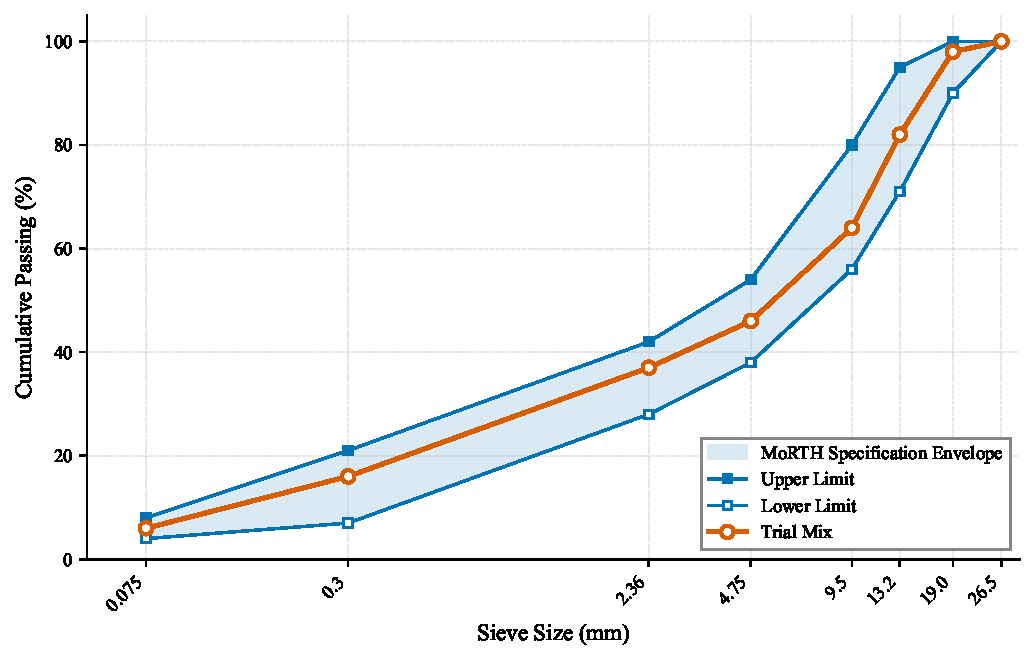
\includegraphics[width=0.9\textwidth]{graphics/gradation_curve.pdf}
    \caption{Aggregate gradation curve for DBM Grading-II with MoRTH specification limits.}
    \label{fig:gradation}
\end{figure}

\subsection{Aggregate Shape Classification}

The shape of coarse aggregates retained on the 12.5\,mm sieve (Material A fraction: 19--12.5\,mm) was characterised using the Zingg diagram classification method. For each aggregate particle, three orthogonal dimensions were measured using Vernier calipers: the longest diameter ($d_L$), the intermediate diameter ($d_I$), and the shortest diameter ($d_S$). Two dimensionless ratios were then calculated:

\begin{equation}
    \text{Elongation Ratio} = \frac{d_I}{d_L}
    \label{eq:elongation}
\end{equation}

\begin{equation}
    \text{Flatness Ratio} = \frac{d_S}{d_I}
    \label{eq:flatness}
\end{equation}

Based on the threshold value of $2/3$ for each ratio, aggregate particles were classified into four shape categories as defined by the Zingg diagram~\cite{teja2020effect}: Cubical (Elongation Ratio $\geq 2/3$ and Flatness Ratio $\geq 2/3$), Rod (Elongation Ratio $< 2/3$ and Flatness Ratio $\geq 2/3$), Disk (Elongation Ratio $\geq 2/3$ and Flatness Ratio $< 2/3$), and Blade (Elongation Ratio $< 2/3$ and Flatness Ratio $< 2/3$). The Zingg classification scheme is illustrated in Figure~\ref{fig:zingg}.

Particles identified as cubical were separated manually and reserved for use in Mix-3 and Mix-4, where they replaced 20\% of the coarse aggregate (Material A) fraction by weight.

\begin{figure}[htbp]
    \centering
    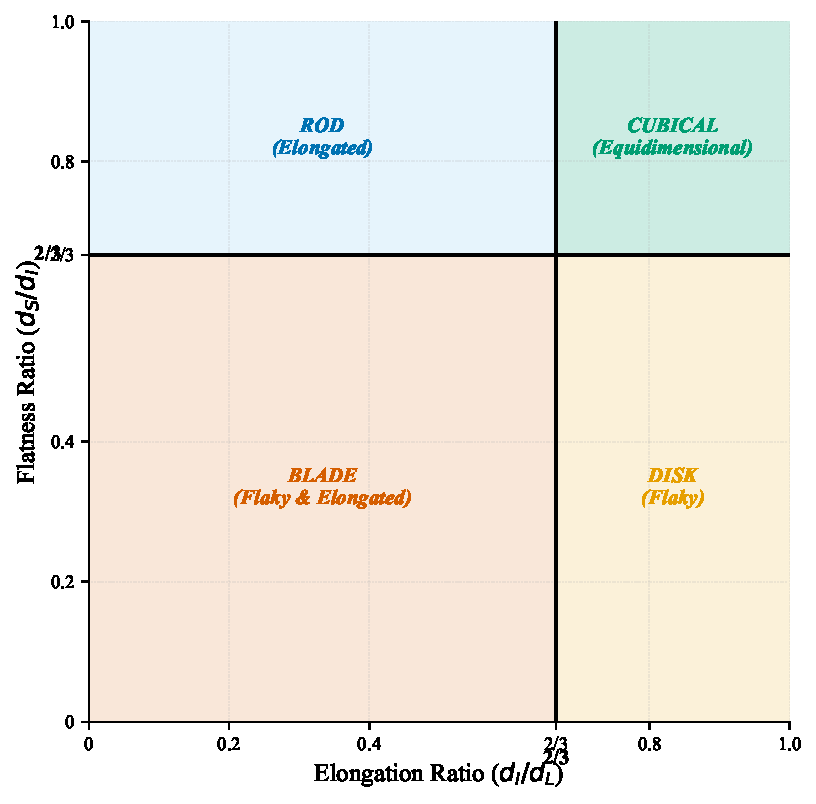
\includegraphics[width=0.7\textwidth]{graphics/zingg_diagram.pdf}
    \caption{Zingg diagram for aggregate shape classification based on elongation ratio and flatness ratio.}
    \label{fig:zingg}
\end{figure}

\subsection{Mix Design}

\subsubsection{Mix Combinations}

Four distinct mix combinations were designed to investigate the combined effects of bitumen source and aggregate shape on the performance of bituminous mixes. The experimental matrix is presented in Table~\ref{tab:mix_matrix}.

\begin{table}[htbp]
    \centering
    \caption{Experimental mix design matrix.}
    \label{tab:mix_matrix}
    \begin{tabular}{@{}clll@{}}
        \toprule
        \textbf{Mix} & \textbf{Bitumen Source} & \textbf{Aggregate Type} & \textbf{Purpose} \\
        \midrule
        Mix-1 & Local (Eastern Refinery) & Natural (as-received) & Control + OBC determination \\
        Mix-2 & Imported (low-cost) & Natural (as-received) & Imported bitumen control \\
        Mix-3 & Local (Eastern Refinery) & 20\% cubical replacement & Shape effect (local) \\
        Mix-4 & Imported (low-cost) & 20\% cubical replacement & Shape effect (imported) \\
        \bottomrule
    \end{tabular}
\end{table}

\subsubsection{Specimen Preparation}

The total batch weight for each specimen was 1200\,g. In compliance with the Ministry of Road Transport and Highways (MoRTH) specifications for Dense Bituminous Macadam (DBM) Grading-II, the material proportioning was established as detailed in Section~\ref{subsec:agg_gradation}: 55\% coarse aggregate, 43\% fine aggregate, and 2\% mineral filler. The aggregates were heated in an oven at 150--170$^{\circ}$C prior to mixing. The bitumen binder was heated separately to 150$^{\circ}$C to achieve the requisite mixing viscosity. The heated aggregate and the designated quantity of bitumen (at the optimum binder content) were combined and mixed thoroughly until all aggregate particles were uniformly coated.

The mix was transferred into a preheated Marshall mould (101.6\,mm diameter) and rodded with a spatula to ensure elimination of entrapped air. Compaction was performed using the Marshall hammer, applying 75 blows on each face of the specimen. The 75-blow compaction effort corresponds to the MoRTH specification for heavy-traffic pavements~\cite{rajkumar2018experimental}. The compacted specimens were allowed to cool to room temperature before extraction from the mould.

\subsubsection{Optimum Binder Content Determination}

The Optimum Binder Content (OBC) was determined exclusively from Mix-1 (local bitumen with natural aggregates), which served as the control mix. Five trial bitumen contents were investigated: 4.0\%, 4.5\%, 5.0\%, 5.5\%, and 6.0\% by weight of the total mix. For each trial bitumen content, three replicate specimens were prepared and tested for Marshall stability, flow, bulk specific gravity, and air voids.

The OBC was determined as the average of the bitumen contents corresponding to: (i) maximum Marshall stability, (ii) maximum bulk specific gravity, and (iii) 4\% design air voids. The resulting OBC was found to be \textbf{5.0\%}. This OBC value was subsequently adopted for the preparation of all remaining mixes (Mix-2, Mix-3, and Mix-4) to ensure a consistent basis for comparison.

\subsection{Testing Programme}

\subsubsection{Marshall Stability and Flow Test}

The Marshall stability and flow test was conducted in accordance with ASTM D6927 / AASHTO T245. For each of the four mix combinations, three replicate specimens were prepared at the OBC of 5.0\%. Prior to testing, the specimens were conditioned in a water bath maintained at 60$^{\circ}$C for a period of 30--40 minutes. The Marshall stability (maximum load sustained by the specimen in kN) and the corresponding flow value (deformation at maximum load in mm) were recorded.

\subsubsection{Volumetric Analysis}

The volumetric properties of the compacted specimens were determined for all four mixes. The following parameters were calculated:

\begin{itemize}
    \item Bulk Specific Gravity ($G_{mb}$)
    \item Air Voids ($V_a$, \%)
    \item Voids in Mineral Aggregate (VMA, \%)
    \item Voids Filled with Bitumen (VFB, \%)
\end{itemize}

\subsection{Summary of Test Matrix}

Table~\ref{tab:test_matrix} summarises the experimental test matrix adopted in this study. A total of 12 Marshall specimens were prepared across the four mix combinations for the performance testing at the optimum binder content.

\begin{table}[htbp]
    \centering
    \caption{Summary of the experimental test matrix.}
    \label{tab:test_matrix}
    \begin{tabular}{@{}lccc@{}}
        \toprule
        \textbf{Test} & \textbf{Specimens per Mix} & \textbf{Number of Mixes} & \textbf{Total Specimens} \\
        \midrule
        Marshall Stability \& Flow & 3 & 4 & 12 \\
        \midrule
        \textbf{Grand Total} & & & \textbf{12} \\
        \bottomrule
    \end{tabular}
\end{table}


\section{Results and Discussion}

\subsection{Properties of Aggregates}

The physical and mechanical properties of the coarse aggregates, sourced from a local quarry in the Sylhet region of Bangladesh, were evaluated against specification limits. The results are presented against their respective maximum specification limits without cross-variant comparison because a single source of natural crushed stone was utilised. 

As illustrated in Figure~\ref{fig:agg_properties}, the Aggregate Impact Value (AIV) and Aggregate Crushing Value (ACV) of the Sylhet quarry aggregates were 18\% and 20\%, respectively, satisfying the required maximum limits of 27\% and 30\%. The Flakiness Index (15\%) and Elongation Index (23\%) were within the maximum limit of 30\%, indicating that the base aggregate shape characteristics meet the requirements prior to any manual shape-sorting.

\begin{figure}[htbp]
    \centering
    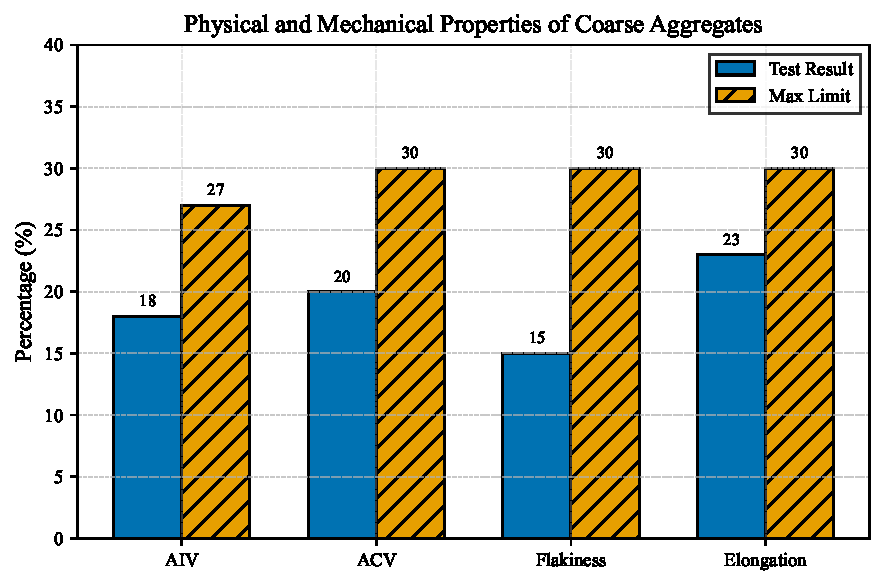
\includegraphics[width=0.7\textwidth]{graphics/aggregate_properties.pdf}
    \caption{Physical and mechanical properties of coarse aggregates compared with maximum specification limits.}
    \label{fig:agg_properties}
\end{figure}

\subsection{Properties of Bituminous Binders}

In Bangladesh's road infrastructure sector, imported bitumen is used to meet demand that exceeds local production capacities. Because the quality of these imported binders varies, which can lead to pavement distresses such as rutting and thermal cracking, a comparative evaluation against the locally produced Eastern Refinery Limited (ERL) bitumen was conducted to quantify the differences.

The physical properties of the locally produced (ERL) and imported bitumen were evaluated and compared graphically in Figure~\ref{fig:bitumen_properties}. The local ERL bitumen exhibited a higher specific gravity (1.023) compared to the imported bitumen (0.99). The softening point of the local binder (52$^{\circ}$C) was higher than that of the imported variant (41$^{\circ}$C), indicating greater resistance to high-temperature deformation.

The flash point (255$^{\circ}$C) and fire point (312$^{\circ}$C) of the local bitumen were higher than those of the imported binder (218$^{\circ}$C and 253$^{\circ}$C, respectively). The ductility of the local bitumen was measured at 112\,cm, compared to 91\,cm for the imported bitumen. The local ERL bitumen met or exceeded the testing requirements across the evaluated rheological and physical parameters.

\begin{figure}[htbp]
    \centering
    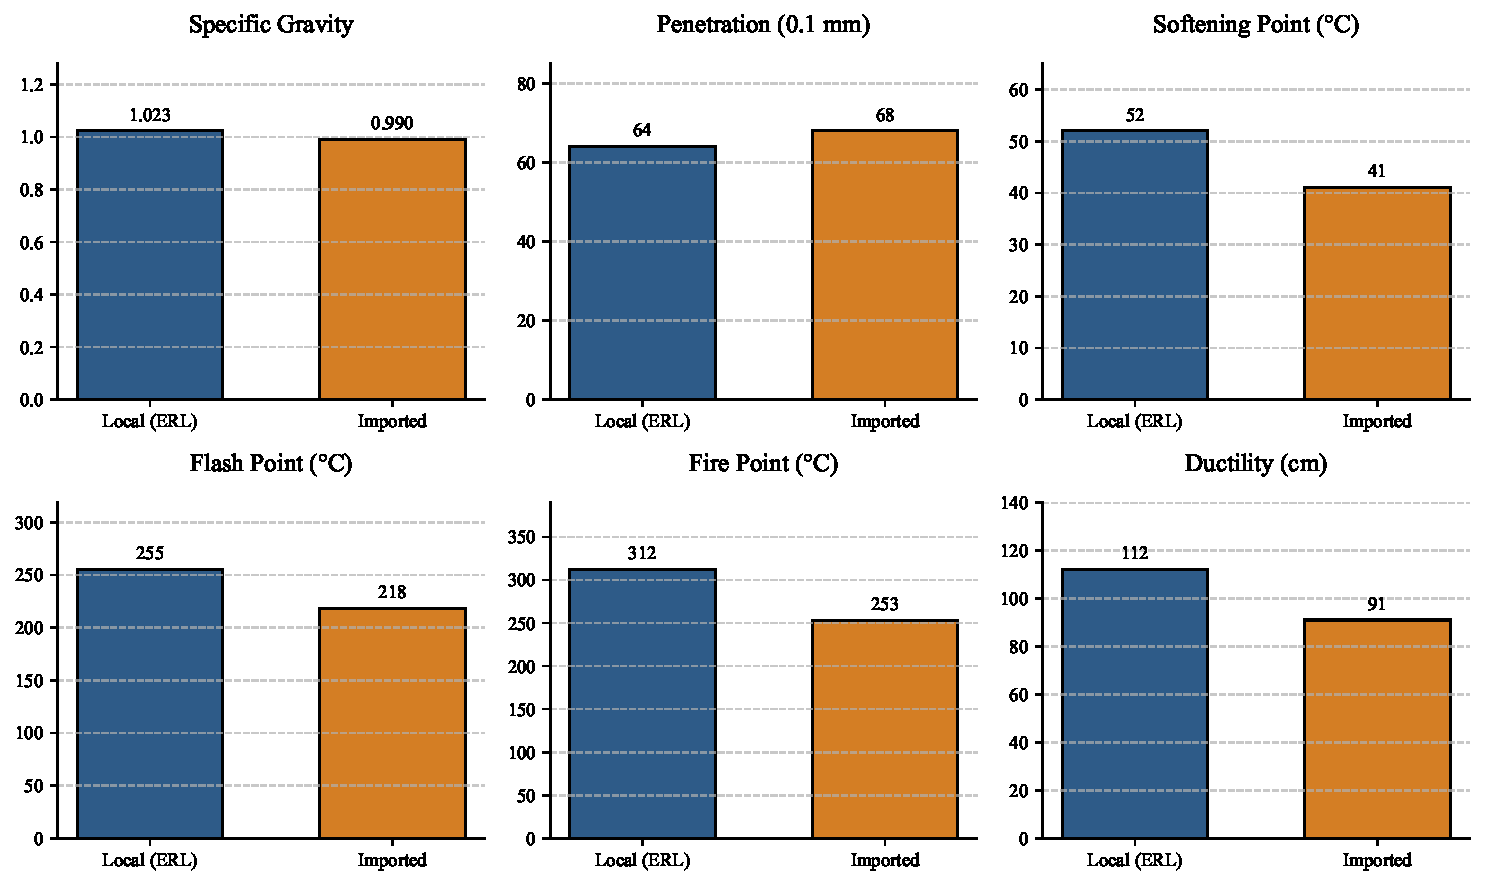
\includegraphics[width=.85\textwidth]{graphics/bitumen_properties.pdf}
    \caption{Graphical comparison of physical properties between local (ERL) and imported low-cost bitumen.}
    \label{fig:bitumen_properties}
\end{figure}

\noindent\textbf{Regional Comparative Assessment (South Asia):}
A comparative assessment of the tested binders against the national highway specifications of neighbouring South Asian countries (India, Pakistan, and Nepal) is detailed in Table~\ref{tab:regional_comparison} and illustrated in Figure~\ref{fig:bitumen_regional_comparison}. The local ERL bitumen, with a Softening Point of $52^{\circ}\text{C}$, satisfies the requirements of Pakistan's NHA ($48$--$56^{\circ}\text{C}$), Nepal's DOR ($48$--$56^{\circ}\text{C}$), and India's MORT\&H (minimum $47^{\circ}\text{C}$). The imported bitumen exhibited a Softening Point of $41^{\circ}\text{C}$, which is below the minimum standards of these regional highway authorities.

The Flash Point of the imported bitumen ($218^{\circ}\text{C}$) does not meet the minimum safety threshold of $232^{\circ}\text{C}$ specified across Bangladesh, India, Nepal, and Pakistan. The local ERL bitumen has a Flash Point of $255^{\circ}\text{C}$, exceeding this threshold. The comparison indicates that the imported bitumen tested does not meet the regional specifications for flexible pavements.

\begin{table}[htbp]
    \centering
    \caption{Comparative analysis of physical properties between experimental bitumen and South Asian standards.}
    \label{tab:regional_comparison}
    \renewcommand{\arraystretch}{1.3}
    \resizebox{\textwidth}{!}{%
    \begin{tabular}{@{}lccccccc@{}}
        \toprule
        \multirow{2}{*}{\textbf{Property}} & \multicolumn{2}{c}{\textbf{Experimental Data}} & \multicolumn{4}{c}{\textbf{National Specifications (60/70 Grade)}} & \multirow{2}{*}{\textbf{Standard}} \\
        \cmidrule(lr){2-3} \cmidrule(lr){4-7}
        & \textbf{Local (ERL)} & \textbf{Imported} & \textbf{RHD (BD)} & \textbf{MORT\&H (IN)} & \textbf{DOR (NP)} & \textbf{NHA (PK)} & \\
        \midrule
        Penetration (dmm) & 64 & 68 & 60--70 & 60--70 & 60--70 & 60--70 & ASTM D5 \\
        Softening Point ($^\circ$C) & 52 & \textbf{41} & 48--56 & 47--55 & 48--56 & 48--56 & ASTM D36 \\
        Ductility (cm) & 112 & \textbf{91} & $\geq$100 & $\geq$75 & $\geq$100 & $\geq$100 & ASTM D113 \\
        Flash Point ($^\circ$C) & 255 & \textbf{218} & $\geq$232 & $\geq$232 & $\geq$232 & $\geq$232 & ASTM D92 \\
        Specific Gravity & 1.023 & \textbf{0.990} & 1.01--1.06 & 1.01--1.06 & 1.01--1.06 & 1.01--1.06 & ASTM D70 \\
        \bottomrule
        \multicolumn{8}{@{}l@{}}{\small Note: Bold values indicate the imported bitumen failed to meet the specified minimum regional requirements.} \\
    \end{tabular}%
    }
\end{table}

\begin{figure}[htbp]
    \centering
    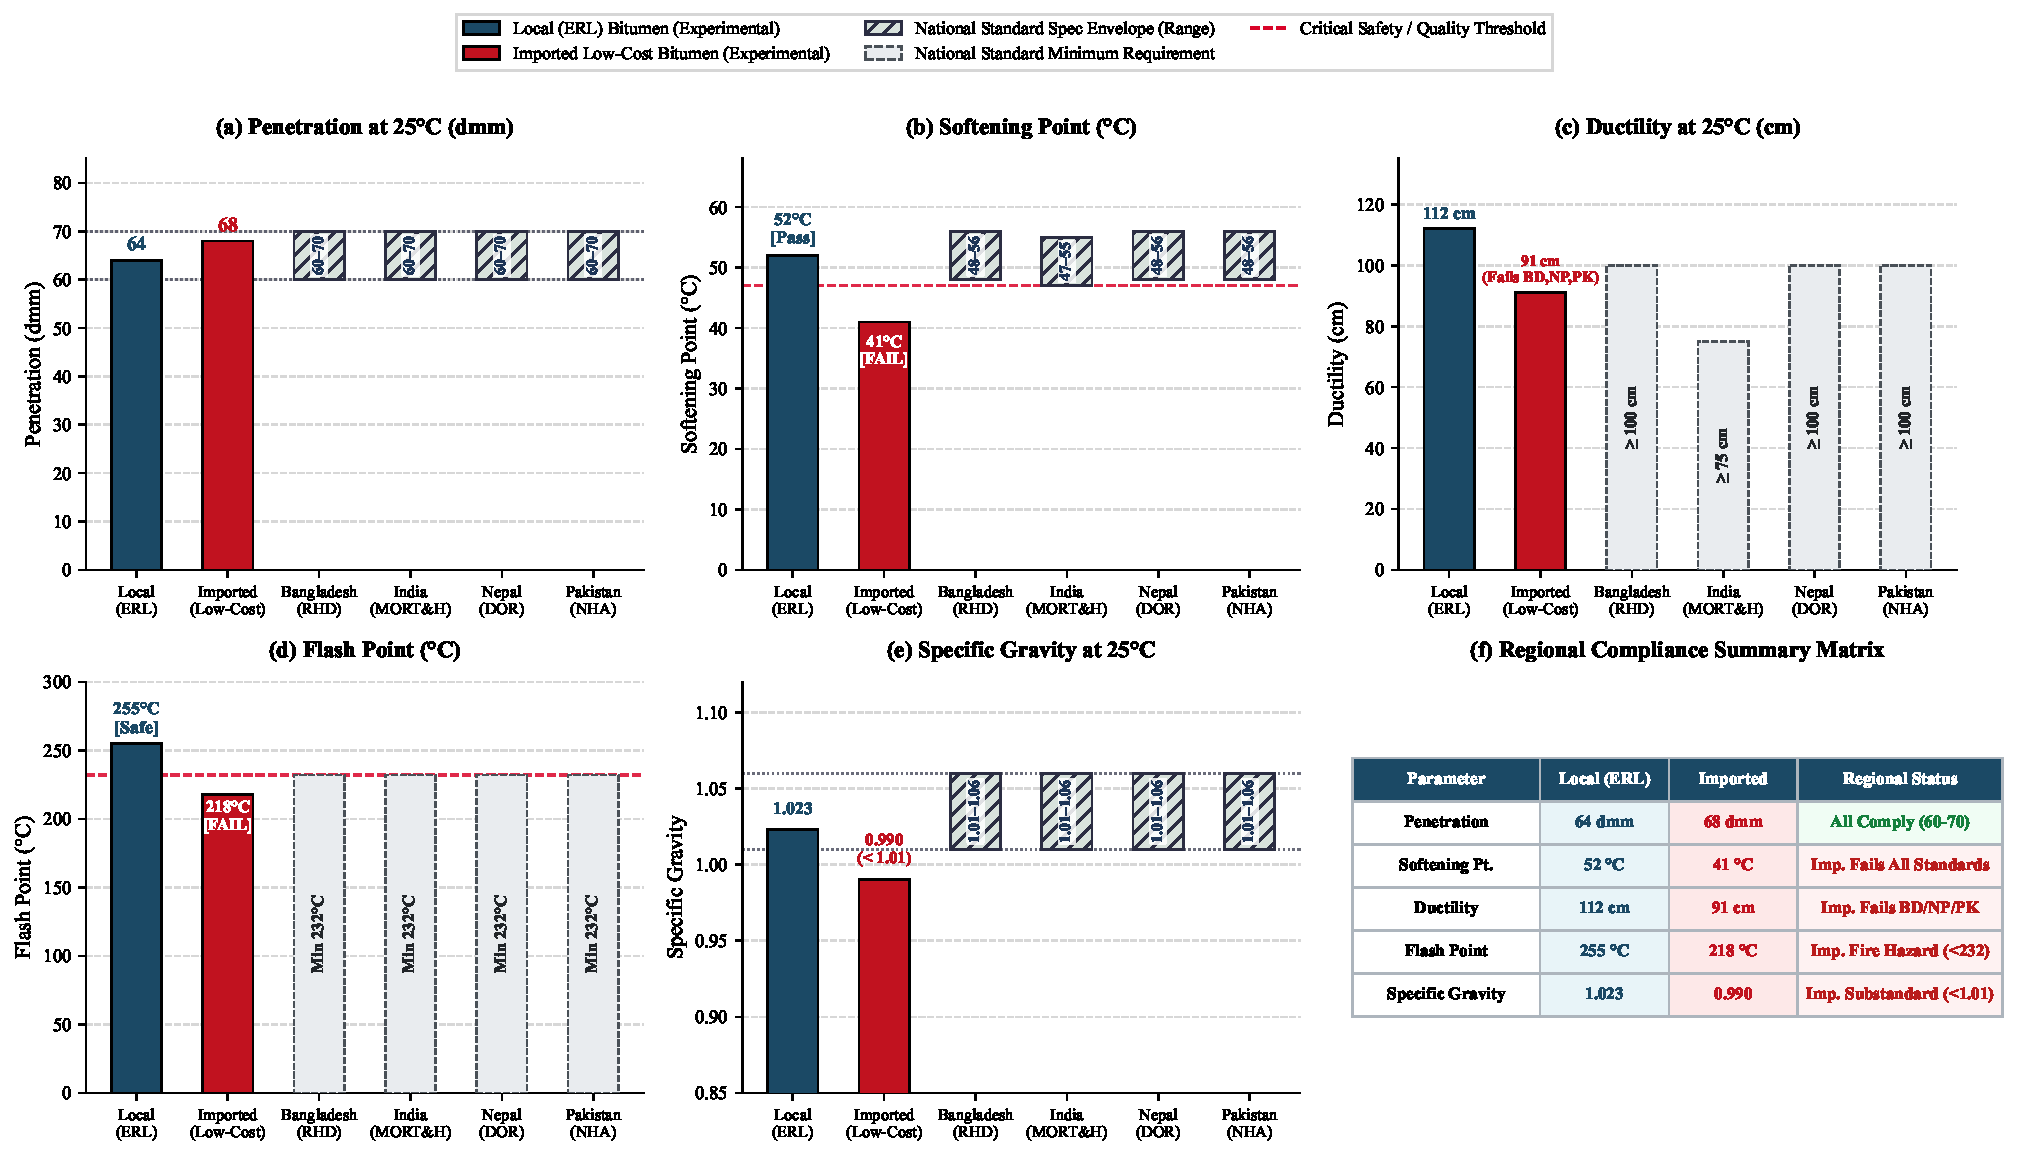
\includegraphics[width=\textwidth]{graphics/bitumen_regional_comparison.pdf}
    \caption{Comparative analysis of experimental physical properties of local (ERL) and imported low-cost bitumen against national highway specifications of South Asian countries (Bangladesh RHD, India MORT\&H, Nepal DOR, and Pakistan NHA).}
    \label{fig:bitumen_regional_comparison}
\end{figure}

\subsection{Determination of Optimum Binder Content}

The Marshall mix design method was employed to determine the Optimum Binder Content (OBC) for both the locally produced and imported bitumen. Specimens were prepared at varying asphalt contents ranging from 4.0\% to 6.0\% in 0.5\% increments. The volumetric properties (air voids, VMA, VFA) and mechanical properties (Marshall stability, flow, and unit weight) were evaluated to establish the optimal mix proportions. 

As detailed in Table~\ref{tab:obc_data} and illustrated in Figure~\ref{fig:obc_determination}, the stability for both binders reached a peak before declining at higher binder contents, while the flow value increased monotonically. The target air void content ($V_a$) of 4.0\%, a standard criterion for heavy traffic pavements, corresponded to an asphalt content of approximately 5.0\% for both the local and imported bitumen mixes. At this 5.0\% OBC, all other volumetric and mechanical parameters, including VMA, VFA, and unit weight, satisfactorily met the Roads and Highways Department (RHD) specification limits. Therefore, 5.0\% was selected as the OBC for the subsequent comparative performance evaluations.

The following fundamental equations were utilised to compute the volumetric properties of the Marshall specimens:
\begin{align}
    G_{mb} &= \frac{W_a}{W_{ssd} - W_w} \\
    G_{mm} &= \frac{P_{mm}}{\frac{P_s}{G_{se}} + \frac{P_b}{G_b}} \\
    P_s &= 100 - P_b \\
    P_{mm} &= 100 \\
    G_{se} &= \frac{P_{mm} - P_b}{\frac{P_{mm}}{G_{mm}} - \frac{P_b}{G_b}} \\
    G_{sb} &= \frac{P_1 + P_2 + P_3}{\frac{P_1}{G_1} + \frac{P_2}{G_2} + \frac{P_3}{G_3}} \\
    V_a (\%) &= 100 \times \frac{G_{mm} - G_{mb}}{G_{mm}} \\
    \text{VMA} (\%) &= 100 - \frac{G_{mb} \times P_s}{G_{sb}} \\
    \text{VFA} (\%) &= \frac{\text{VMA} - V_a}{\text{VMA}} \times 100
\end{align}
where $W_a$ is the weight of the specimen in air, $W_{ssd}$ is the saturated surface dry weight, $W_w$ is the weight in water, $P_b$ is the percent of binder by total weight of mix, $P_s$ is the percent of aggregate, $G_b$ is the specific gravity of the binder, $G_{se}$ is the effective specific gravity of the aggregate, $G_{sb}$ is the bulk specific gravity of the aggregate blend (with $P_1, P_2, P_3$ and $G_1, G_2, G_3$ being the percentages and specific gravities of the individual aggregate fractions), $G_{mm}$ is the theoretical maximum specific gravity of the mixture, and $G_{mb}$ is the bulk specific gravity of the compacted mixture.

\begin{table}[htbp]
    \centering
    \caption{Marshall mix design properties for Optimum Binder Content determination.}
    \label{tab:obc_data}
    \resizebox{\textwidth}{!}{
    \begin{threeparttable}
    \begin{tabular}{lccccccccccccccccc}
        \toprule
        \textbf{Bitumen Type} & \textbf{AC} & \textbf{$W_a$} & \textbf{$W_w$} & \textbf{$W_{ssd}$} & \textbf{$G_{mb}$} & \textbf{$\gamma$} & \textbf{$G_{mm}$} & \textbf{$P_s$} & \textbf{$G_{sb}$} & \textbf{$V_a$} & \textbf{VMA} & \textbf{VFA} & \textbf{$H$} & \textbf{CF} & \textbf{$S_{obs}$} & \textbf{$S_{cor}$} & \textbf{$F$} \\
        \midrule
        \multirow{5}{*}{\textbf{Local (ERL)}} 
        & 4.0 & 1176.5 & 677.4 & 1181.2 & 2.330 & 145.72 & 2.520 & 96.0 & 2.684 & 7.54 & 16.66 & 54.75 & 65.0 & 0.932 & 1946 & 1813.67 & 9.5 \\
        & 4.5 & 1216.6 & 704.7 & 1230.2 & 2.315 & 144.46 & 2.501 & 95.5 & 2.684 & 7.44 & 17.44 & 57.81 & 65.0 & 0.932 & 2625 & 2446.50 & 9.0 \\
        & 5.0 & 1202.3 & 696.9 & 1206.3 & 2.360 & 147.28 & 2.482 & 95.0 & 2.684 & 4.92 & 16.47 & 70.15 & 63.5 & 1.000 & 2500 & 2500.00 & 10.0 \\
        & 5.5 & 1221.2 & 715.6 & 1222.3 & 2.410 & 150.38 & 2.464 & 94.5 & 2.684 & 2.19 & 15.15 & 85.54 & 64.3 & 0.950 & 2517 & 2438.60 & 11.0 \\
        & 6.0 & 1230.6 & 722.4 & 1231.3 & 2.418 & 150.89 & 2.445 & 94.0 & 2.684 & 1.10 & 15.32 & 92.79 & 65.0 & 0.932 & 2273 & 2118.40 & 14.0 \\
        \midrule
        \multirow{5}{*}{\textbf{Imported}} 
        & 4.0 & 1199.5 & 690.1 & 1204.2 & 2.333 & 145.58 & 2.520 & 96.0 & 2.684 & 7.42 & 16.55 & 55.17 & 64.5 & 0.946 & 1452 & 1373.81 & 10.0 \\
        & 4.5 & 1205.9 & 691.5 & 1210.7 & 2.323 & 144.96 & 2.501 & 95.5 & 2.684 & 7.12 & 17.35 & 58.97 & 64.6 & 0.944 & 1133 & 1069.42 & 11.0 \\
        & 5.0 & 1206.7 & 701.6 & 1208.6 & 2.380 & 148.51 & 2.482 & 95.0 & 2.684 & 4.11 & 15.76 & 73.92 & 63.4 & 1.003 & 1909 & 1913.51 & 11.0 \\
        & 5.5 & 1225.7 & 715.8 & 1226.8 & 2.399 & 149.70 & 2.464 & 94.5 & 2.684 & 2.64 & 15.53 & 83.01 & 63.6 & 0.992 & 2045 & 2028.64 & 12.0 \\
        & 6.0 & 1200.0 & 708.1 & 1201.5 & 2.432 & 151.76 & 2.445 & 94.0 & 2.684 & 0.53 & 14.83 & 96.11 & 65.1 & 0.960 & 2274 & 2182.67 & 15.0 \\
        \bottomrule
    \end{tabular}
    \begin{tablenotes}
        \small
        \item \textit{Note:} AC = Asphalt Content (\%); $W_a$ = Specimen weight in air (g); $W_w$ = Specimen weight in water (g); $W_{ssd}$ = Saturated surface dry weight (g); $G_{mb}$ = Bulk specific gravity; $\gamma$ = Unit weight (lb/cft); $G_{mm}$ = Maximum specific gravity; $P_s$ = Percent of aggregate (\%); $G_{sb}$ = Bulk specific gravity of aggregate; $V_a$ = Air voids (\%); VMA = Voids in mineral aggregate (\%); VFA = Voids filled with asphalt (\%); $H$ = Specimen height (mm); CF = Correction factor; $S_{obs}$ = Observed stability (lbs); $S_{cor}$ = Corrected stability (lbs); $F$ = Flow (0.25\,mm).
    \end{tablenotes}
    \end{threeparttable}
    }
\end{table}

\begin{figure}[H]
    \centering
    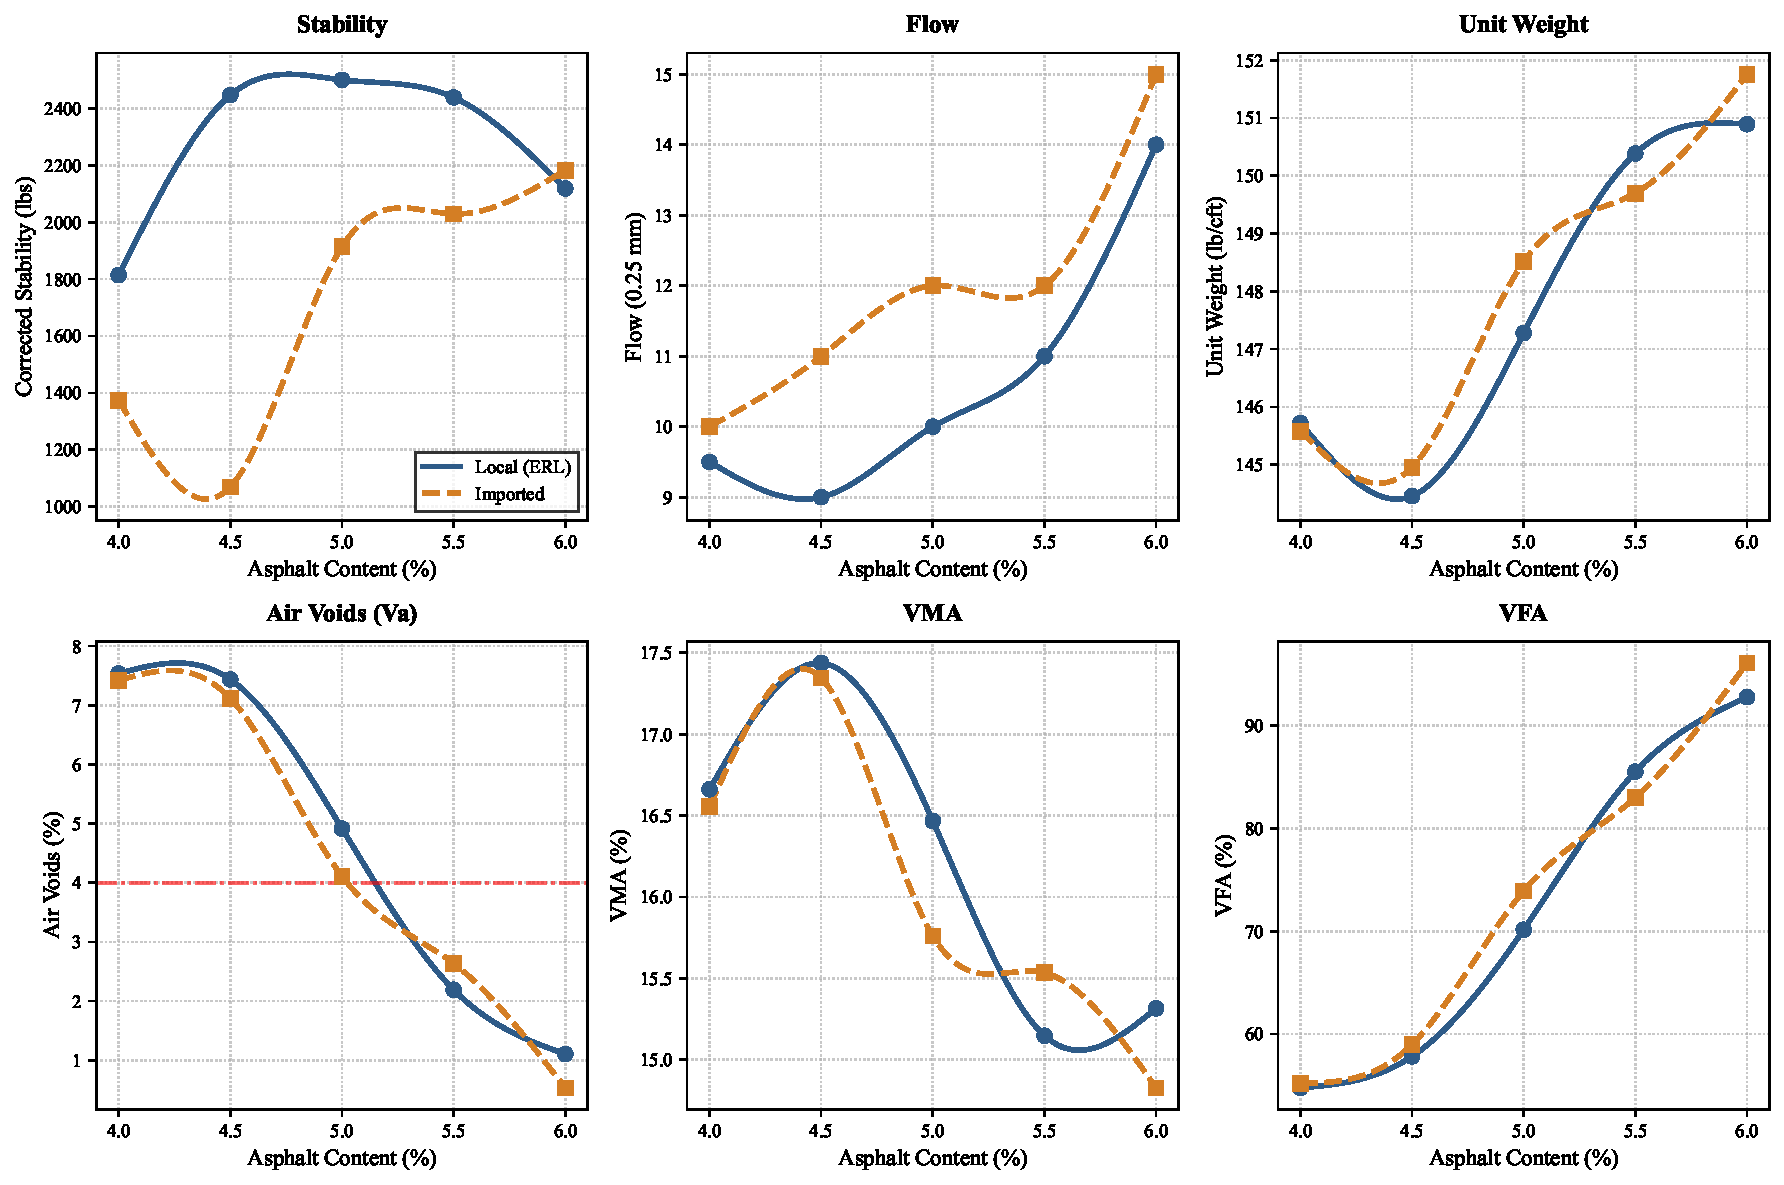
\includegraphics[width=\textwidth]{graphics/obc_determination.pdf}
    \caption{Marshall mix design properties across varying asphalt contents for Optimum Binder Content (OBC) determination.}
    \label{fig:obc_determination}
\end{figure}

\subsection{Comparative Analysis of Bituminous Mixtures}

Following the determination of the 5.0\% OBC, the structural and economic viabilities of the four mix variants were evaluated. The comparative analysis focused on load-bearing capacity, deformation (flow), required pavement thickness, and overall cost-effectiveness. The raw Marshall properties of the four variants are summarized in Table~\ref{tab:mix_data}, while the interaction effects between the binder type (Local vs. Imported) and aggregate shape (Normal vs. 20\% Cubical) are graphically illustrated in Figure~\ref{fig:mix_comparison}.

\begin{table}[htbp]
    \centering
    \caption{Comparative Marshall properties of the four bituminous mix variants evaluated at 5.0\% OBC.}
    \label{tab:mix_data}
    \resizebox{\textwidth}{!}{
    \begin{threeparttable}
    \begin{tabular}{lccccccccccccccccc}
        \toprule
        \textbf{Variant} & \textbf{OBC} & \textbf{$W_a$} & \textbf{$W_w$} & \textbf{$W_{ssd}$} & \textbf{$G_{mb}$} & \textbf{$\gamma$} & \textbf{$G_{mm}$} & \textbf{$P_s$} & \textbf{$G_{sb}$} & \textbf{$V_a$} & \textbf{VMA} & \textbf{VFA} & \textbf{$H$} & \textbf{CF} & \textbf{$S_{obs}$} & \textbf{$S_{cor}$} & \textbf{$F$} \\
        \midrule
        Local + Normal & 5.0 & 1168.9 & 688.5 & 1176.0 & 2.398 & 149.64 & 2.479 & 95.0 & 2.680 & 3.27 & 15.00 & 78.20 & 61.9 & 1.040 & 1883 & 1958.81 & 10.0 \\
        Imp + Normal & 5.0 & 1176.8 & 679.7 & 1181.0 & 2.348 & 146.52 & 2.469 & 95.0 & 2.680 & 4.90 & 16.77 & 70.78 & 64.6 & 0.994 & 1126 & 1119.40 & 17.0 \\
        Local + 20\% Cubical & 5.0 & 1180.2 & 684.3 & 1186.0 & 2.350 & 146.64 & 2.479 & 95.0 & 2.680 & 5.20 & 16.70 & 68.86 & 60.3 & 1.090 & 2744 & 2990.55 & 8.5 \\
        Imp + 20\% Cubical & 5.0 & 1250.3 & 733.2 & 1253.0 & 2.405 & 150.07 & 2.469 & 95.0 & 2.680 & 2.59 & 14.93 & 82.65 & 65.1 & 0.960 & 2156 & 2070.13 & 12.0 \\
        \bottomrule
    \end{tabular}
    \begin{tablenotes}
        \small
        \item \textit{Note:} See Table~\ref{tab:obc_data} for column abbreviations. OBC = Optimum Binder Content (\%).
    \end{tablenotes}
    \end{threeparttable}
    }
\end{table}

\textbf{A. Overall Performance Assessment:}

The performance of all four mix combinations was assessed across structural and volumetric parameters. A graphical representation of these parameters---Marshall stability, flow value, unit weight, air voids ($V_a$), voids in mineral aggregate (VMA), and voids filled with asphalt (VFA)---is provided in Figure~\ref{fig:performance_assessment}. The experimental results, detailed in Table~\ref{tab:mix_data}, indicate interactions between the binder source and the morphological properties of the aggregate matrix.

From a volumetric perspective, the spatial arrangement of the aggregate skeleton affects compaction characteristics. The control mixes incorporating normal aggregates (Mix-1 and Mix-2) maintained air voids within standard limits ($3.27\%$ and $4.90\%$, respectively) and exhibited sufficient VMA for durability. However, the introduction of $20\%$ cubical aggregates produced different volumetric responses depending on the bitumen type. The mix comprising imported bitumen and cubical aggregates (Mix-4) resulted in a dense matrix with air voids at $2.59\%$ and a VFA of $82.65\%$. In a subtropical monsoon climate, air void contents below the standard limit increase the risk of binder bleeding and plastic flow under traffic loading~\cite{imran2025developing}. 

In contrast, the combination of local Eastern Refinery (ERL) bitumen with $20\%$ cubical aggregates (Mix-3) achieved a VMA of $16.70\%$, providing space for the binder film thickness, while maintaining an air void content of $5.20\%$. As visualised in Figure~\ref{fig:performance_assessment}, this volumetric state coincided with an increase in shear resistance, yielding a Marshall stability of $2990.55$\,lbs. The comparative unit weights indicate improved densification and aggregate interlock with the cubical fraction. Mix-3 demonstrates that structural capacity can be increased while maintaining volumetric proportions necessary for long-term pavement fatigue life and rutting resistance.

\begin{figure}[H]
    \centering
    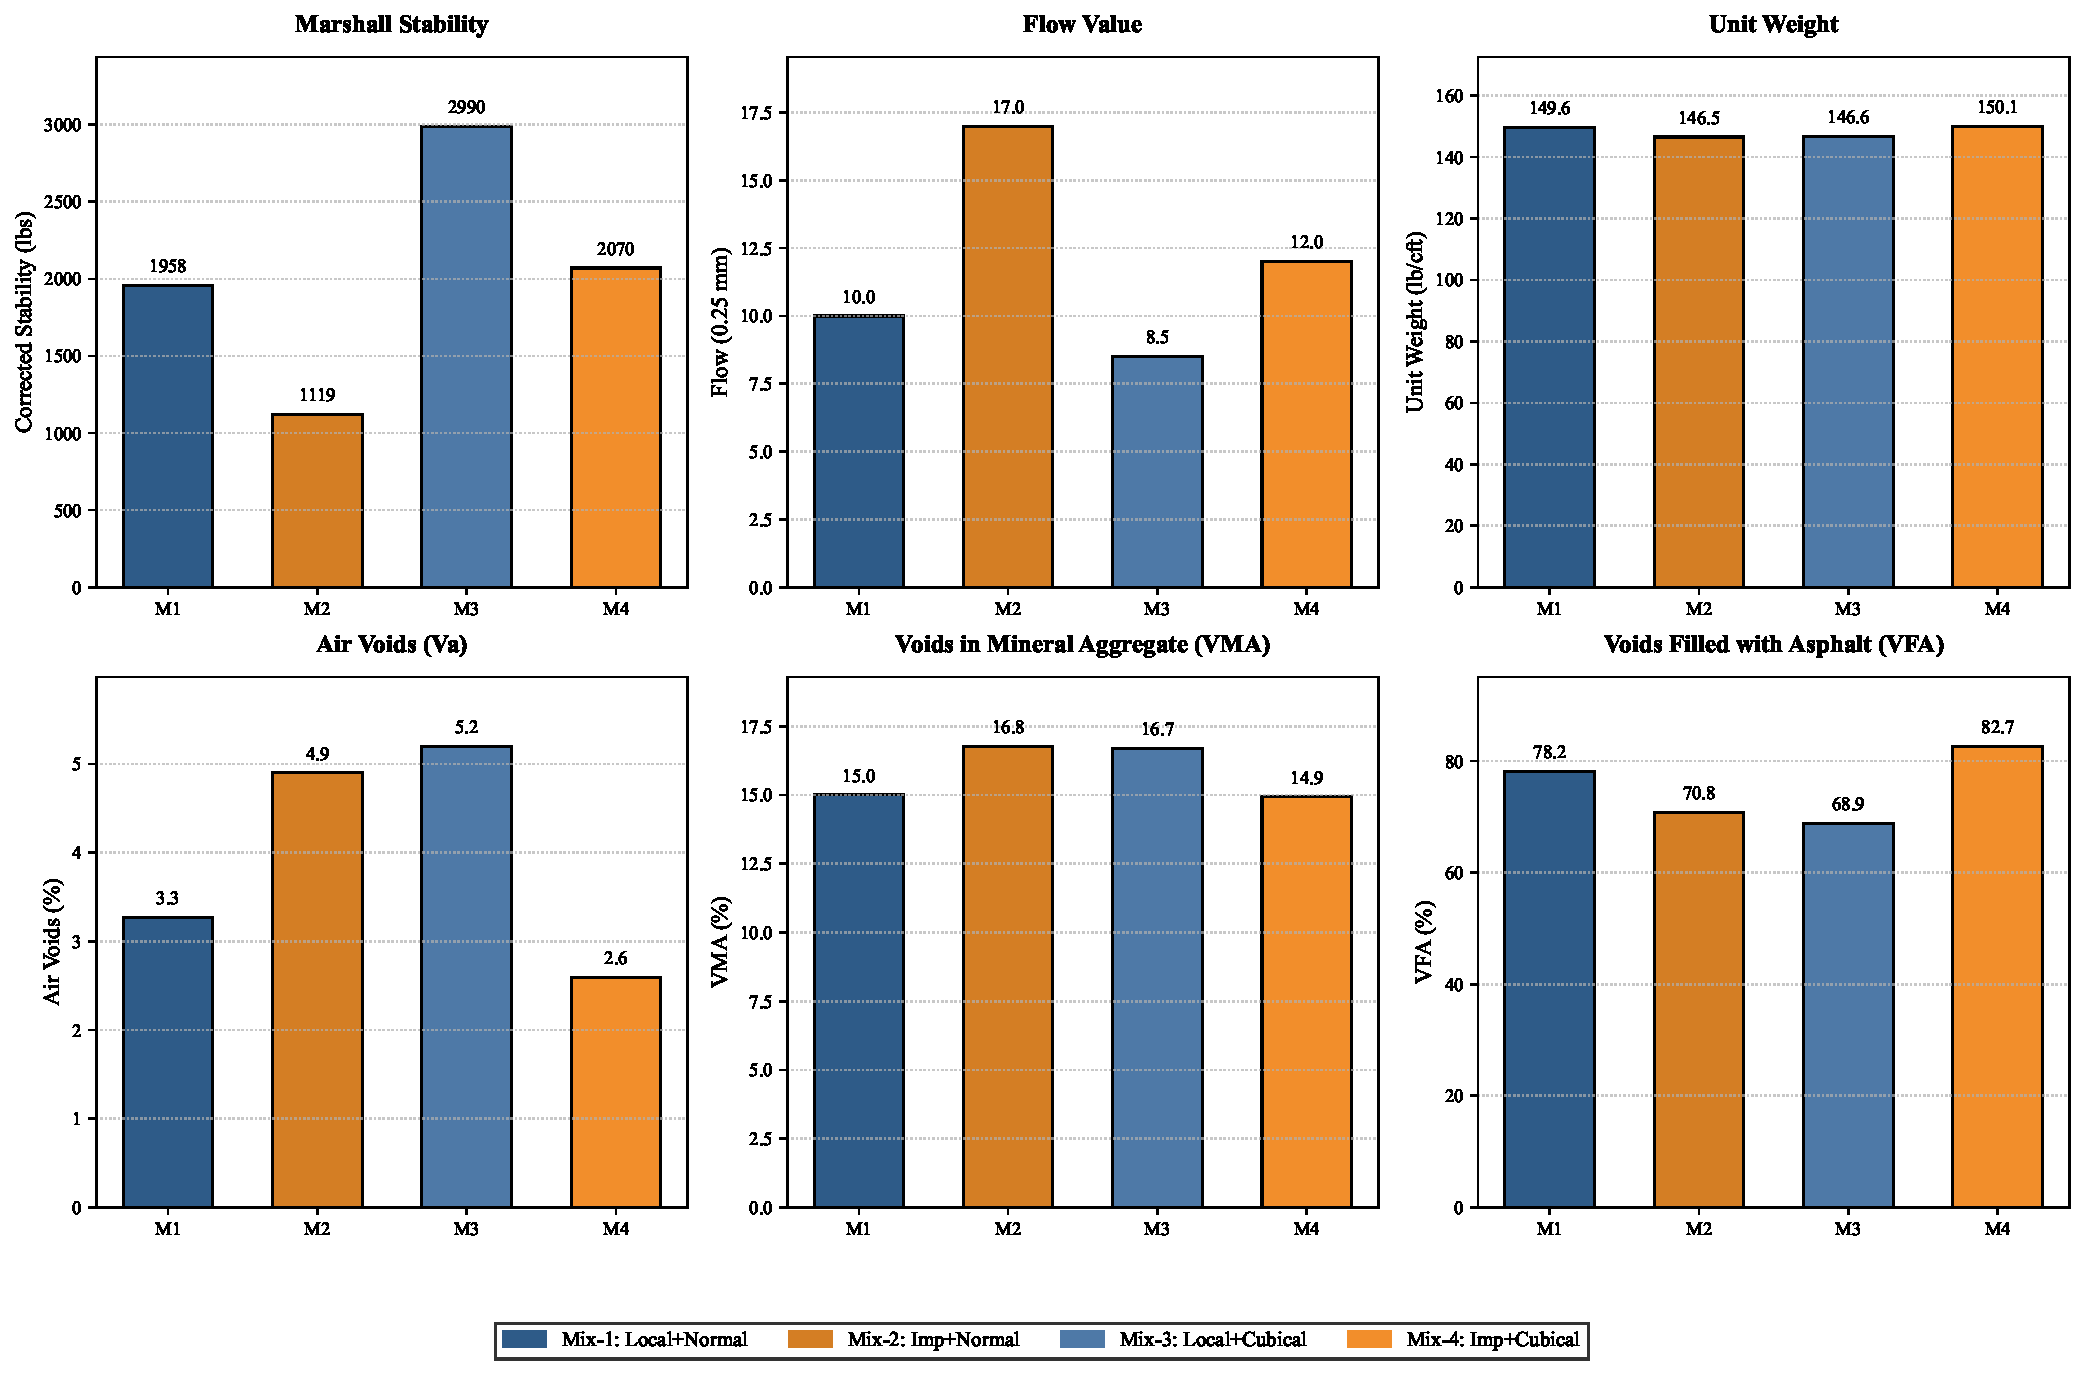
\includegraphics[width=\textwidth]{graphics/performance_assessment.pdf}
    \caption{Comprehensive performance assessment of the four bituminous mix variants across key Marshall stability, flow, and volumetric parameters.}
    \label{fig:performance_assessment}
\end{figure}

\textbf{B. Load Bearing Capacity (Marshall Stability):}
As depicted in the left subplot of Figure~\ref{fig:mix_comparison}, the incorporation of 20\% cubical aggregates increased the load-bearing capacity for both binder types. The mix comprising Local (ERL) bitumen and 20\% cubical aggregates exhibited the highest Marshall stability (2991 lbs). The lower penetration value of the ERL bitumen provided stiffness to the mix. This observation aligns with the findings of Bagampadde et al. (2006) \cite{bagampadde2006impact}, who reported that bitumen with lower penetration grades exhibits higher mechanical strength in bituminous mixes. The Imported bitumen with normal aggregates yielded the lowest stability (1119 lbs).

\textbf{C. Deformation (Flow Value):}
The right subplot of Figure~\ref{fig:mix_comparison} presents the flow characteristics, measured in units of 0.25\,mm. The Imported bitumen with normal aggregates displayed the highest flow (17 units), indicating susceptibility to permanent deformation and rutting under traffic loads. The Local bitumen with 20\% cubical aggregates combination maintained a flow value of 8.5 units, which aligns with the RHD specification limits for heavy-duty pavements.

\textbf{D. Required Pavement Thickness:}
According to the AASHTO structural design guidelines for flexible pavements, the structural layer coefficient ($a_1$) of the bituminous surfacing is proportional to its Marshall stability and resilient modulus. Because the Local bitumen with 20\% cubical aggregates mix achieved the highest stability, it corresponds to the highest $a_1$ value. To achieve a target Structural Number (SN) for a specific traffic load, this mix requires a lesser pavement thickness compared to the other variants. The Imported bitumen mix with normal aggregates would require a thicker asphalt layer due to its lower structural coefficient.

\textbf{E. Cost Effectiveness:}
The required pavement thickness affects the economics of road construction. By achieving the requisite structural capacity with a thinner asphalt layer, the Local bitumen and 20\% cubical aggregates mix reduces the total volume of bituminous materials required per kilometre of road. This material reduction can offset initial costs associated with local refining or aggregate shape-sorting, presenting a cost-effective alternative over the pavement's lifecycle.

\begin{figure}[H]
    \centering
    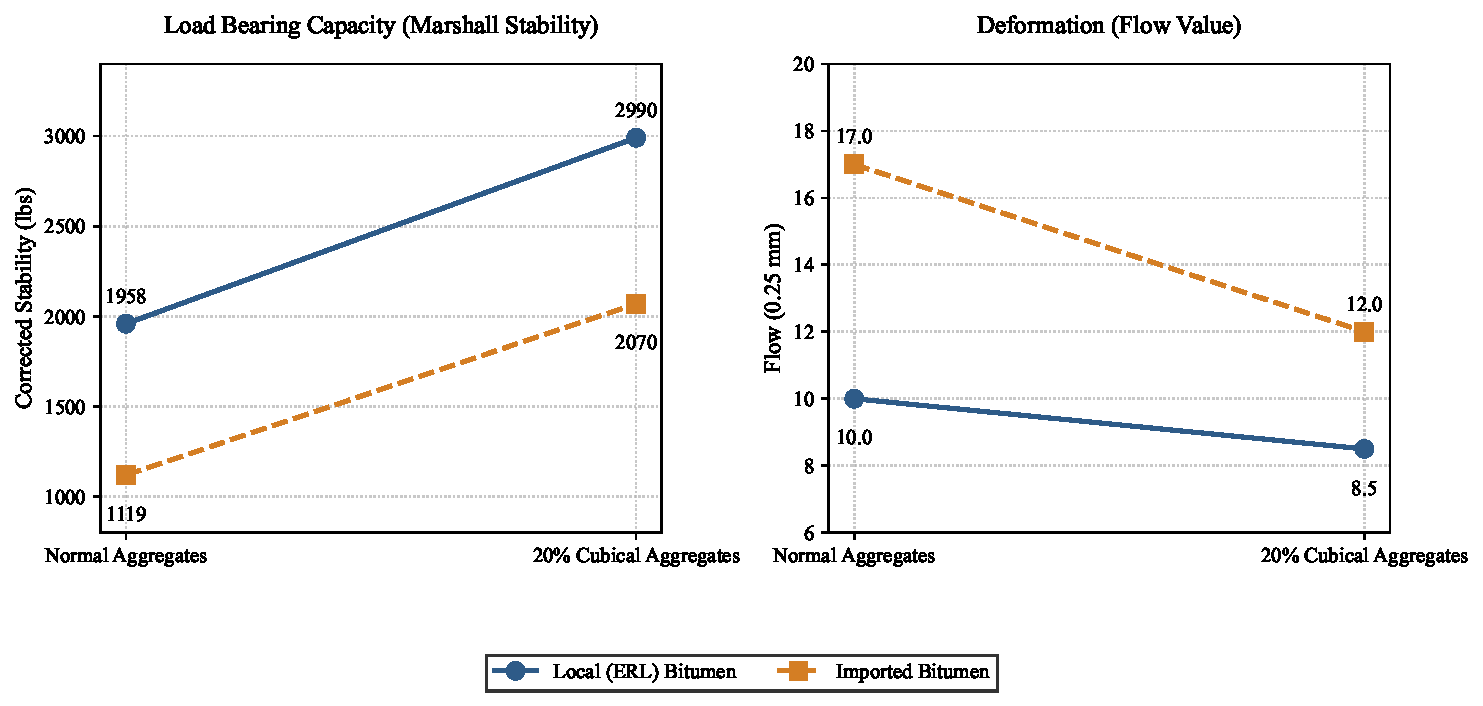
\includegraphics[width=\textwidth]{graphics/mix_comparison.pdf}
    \caption{Interaction line plots comparing Marshall stability and flow across four bituminous mix variants.}
    \label{fig:mix_comparison}
\end{figure}

\subsection{Proposed Roadmap for Cost-Effective Road Construction in Bangladesh}

Road construction costs in Bangladesh are affected by weak subgrade soils, heavy monsoon rainfall, and reliance on imported construction materials. Based on the findings of this study and existing literature, a dual-level strategy is proposed to improve pavement durability and manage construction costs.

The strategy combines subgrade stabilization with optimized surface layer mixtures:

\begin{enumerate}
    \item \textbf{Foundation Level (Subgrade Stabilization):} The subgrade acts as the load-bearing stratum for the pavement structure. In Bangladesh, weak subgrade conditions necessitate thick base and sub-base layers. As reported by Sood and Bansal \cite{sood2015evaluation}, treating weak subgrade soils with industrial by-products such as lime and fly ash increases the California Bearing Ratio (CBR). A stabilized, higher-CBR subgrade provides a platform that reduces the required thickness of overlying flexible pavement layers.
    \item \textbf{Surface Level (Optimized Bituminous Mix):} Building upon the stabilized foundation, the surface course requires resistance to rutting and moisture damage. The experimental results indicated that combining locally produced (ERL) bitumen with 20\% cubical aggregates yielded a Marshall stability of 2991 lbs and a flow value of 8.5 units. This stability translates to a higher structural layer coefficient ($a_1$) in empirical pavement design methodologies (e.g., AASHTO 1993).
\end{enumerate}

\textbf{Techno-Economic Summary:}
By strengthening the foundation using stabilizing agents (lime and fly ash) and utilizing the structural capacity of the optimized asphalt surfacing (ERL bitumen with 20\% cubical aggregates), the required structural number (SN) can be achieved with thinner pavement layers. This reduction in the volume of aggregates and bituminous binders provides a method to lower road construction costs in Bangladesh while maintaining structural integrity.

\section{Conclusion}

\subsection{Summary of Findings}
This study presented a comparative laboratory investigation of locally produced Eastern Refinery bitumen and imported bitumen for road construction applications in Bangladesh, focusing on the influence of aggregate particle shape (20\% cubical replacement). Based on the experimental results of the Marshall mix design and volumetric analyses, the following conclusions are drawn:
\begin{itemize}
    \item The locally refined bitumen from Eastern Refinery Limited (ERL) exhibited rheological properties, including higher viscosity and uniform penetration grades, that met or exceeded testing requirements when compared with the imported binder.
    \item The combination of 20\% cubical aggregates with local ERL bitumen (Mix-3) yielded a Marshall stability of 2991 lbs (13.3 kN) and a flow of 8.5 units.
    \item Volumetric analysis indicated that while conventional mixes maintained properties within standard tolerances, combining imported bitumen with 20\% cubical aggregates (Mix-4) resulted in air voids at 2.59\% and Voids Filled with Asphalt at 82.65\%, increasing the risk of binder bleeding under traffic.
    \item Local ERL bitumen combined with shape-optimised (cubical) aggregates provides a structurally and volumetrically stable bituminous matrix, achieving higher load-bearing capacity without compromising durability.
    \item \textbf{Proposed Roadmap for Bangladesh:} A dual-level strategy is proposed: (1) \textit{Foundation Level:} chemical stabilisation of weak local subgrade soils using industrial by-products to increase CBR; and (2) \textit{Surface Level:} employing local ERL bitumen with shape-optimised (minimum 20\% cubical) aggregates. This approach reduces the total volume of imported materials required.
\end{itemize}

\subsection{Recommendations for Practice}
Based on the experimental evidence, a dual-level strategy is recommended for road infrastructure in Bangladesh:

\begin{enumerate}
    \item \textbf{Foundation Level (Subgrade Stabilization):} To address weak subgrade soils, chemical stabilisation using industrial by-products (e.g., lime or fly ash) is recommended. This approach increases the California Bearing Ratio (CBR), providing a platform that reduces the required thickness of overlying flexible layers.
    \item \textbf{Surface Level (Optimized Bituminous Mix):} The Roads and Highways Department (RHD) should revise material specifications to include quality control on imported bitumen and aggregate shape sorting. Introducing a specification for a minimum threshold of $20\%$ cubical coarse aggregates paired with local ERL bitumen enhances the interlocking matrix. 
\end{enumerate}

Implementing these shifts will increase the structural layer coefficient ($a_1$) of the surfacing course. This integrated approach reduces the total volume of materials required, lowering lifecycle costs for highway projects.

\subsection{Future Work}
The following areas are proposed for future investigation:
\begin{itemize}
    \item \textbf{Indirect Tensile Strength (ITS) Testing:} Conducting ITS tests (ASTM D6931) to evaluate the tensile strength characteristics and fracture resistance of the mix combinations under loading.
    \item \textbf{Moisture Susceptibility and Climate Resistance:} Performing the Retained Stability test (Marshall immersion) or Tensile Strength Ratio (TSR) tests to evaluate the stripping resistance of the mixes under conditions representing Bangladesh's subtropical monsoon climate.
    \item \textbf{Rutting and Fatigue Evaluation:} Conducting the Hamburg Wheel Tracking Test (AASHTO T 324) to evaluate rutting depth progression, and the Four-Point Bending Beam Fatigue Test (AASHTO T 321) to assess the fatigue cracking resistance of the bituminous mixtures under cyclic traffic loading.
    \item \textbf{Evaluation of Polymer Modified Bitumen (PMB):} Future research should investigate the enhancement of these base bitumens by adding 5\% SBS (Styrene-Butadiene-Styrene) polymer to produce Polymer Modified Bitumen (PMB), in accordance with LGED specifications. A comparative study on PMB could evaluate the extent to which polymer modification affects the load-bearing capacity and fatigue life of flexible pavements in this region.
    \item \textbf{Performance Enhancement of Imported Bitumen:} Because importing bitumen remains necessary for Bangladesh, future research could explore the performance enhancement of these imported binders. Future studies should investigate the modification of imported bitumen using additives such as 5\% SBS polymer, crumb rubber, or waste plastics to elevate the structural and rheological properties of imported bitumen.
\end{itemize}

\clearpage
\phantomsection
\addcontentsline{toc}{section}{References}
\bibliographystyle{plain}
\bibliography{biblography}

\clearpage
\section{Appendix}

\begin{center}
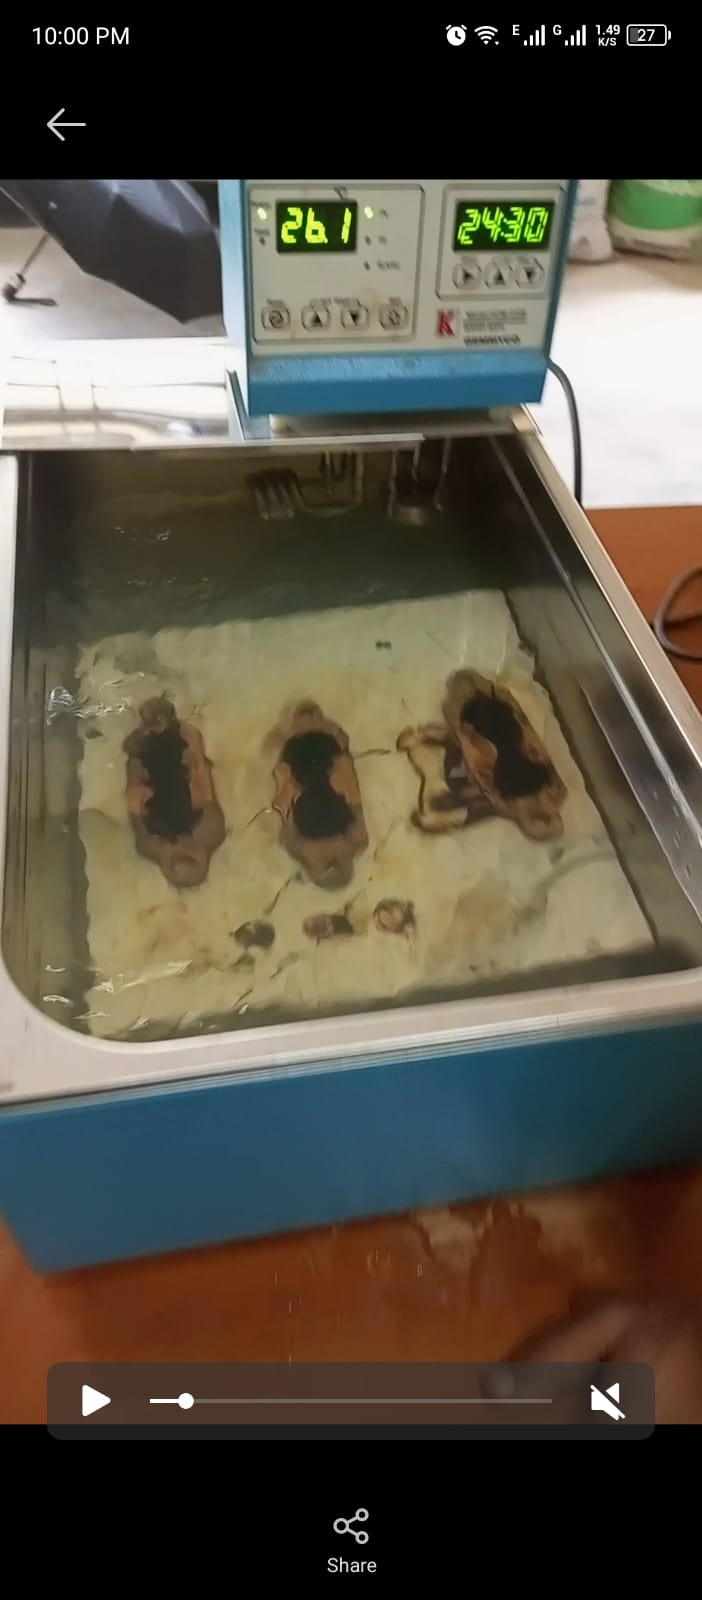
\includegraphics[width=4in, height=4in]{albums/appendix_01.jpeg}
\vspace{0.5cm}

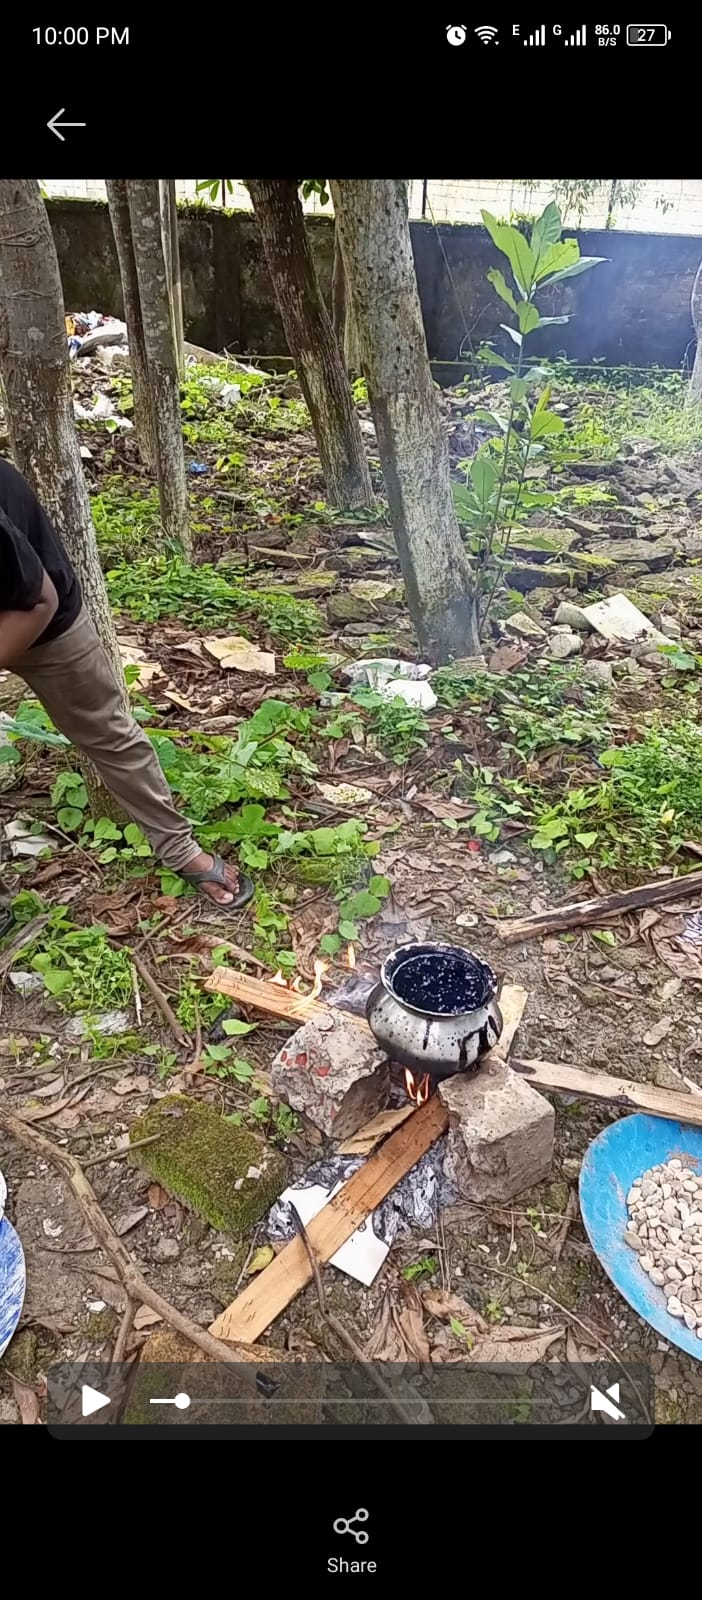
\includegraphics[width=4in, height=4in]{albums/appendix_02.jpeg}
\vspace{0.5cm}

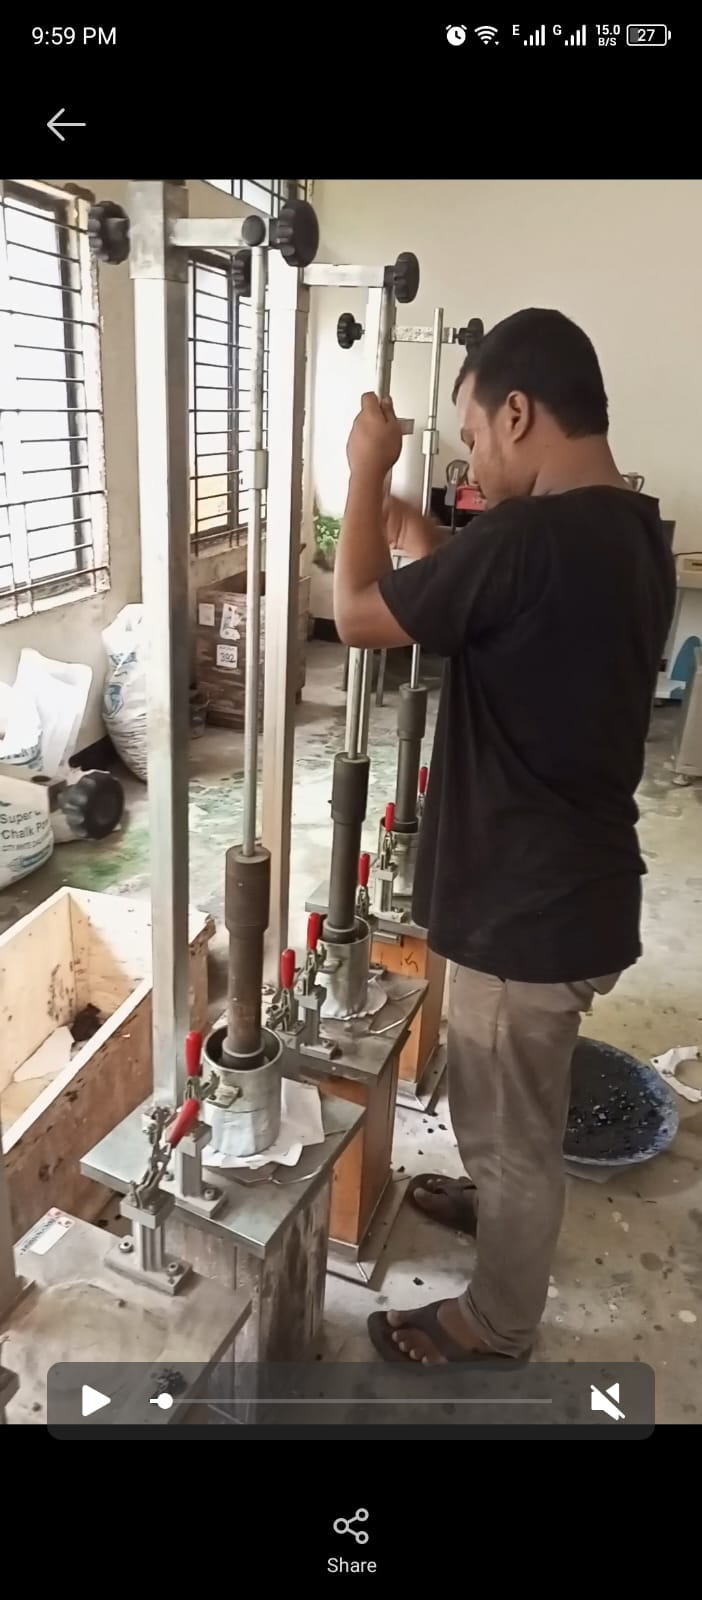
\includegraphics[width=4in, height=4in]{albums/appendix_03.jpeg}
\vspace{0.5cm}

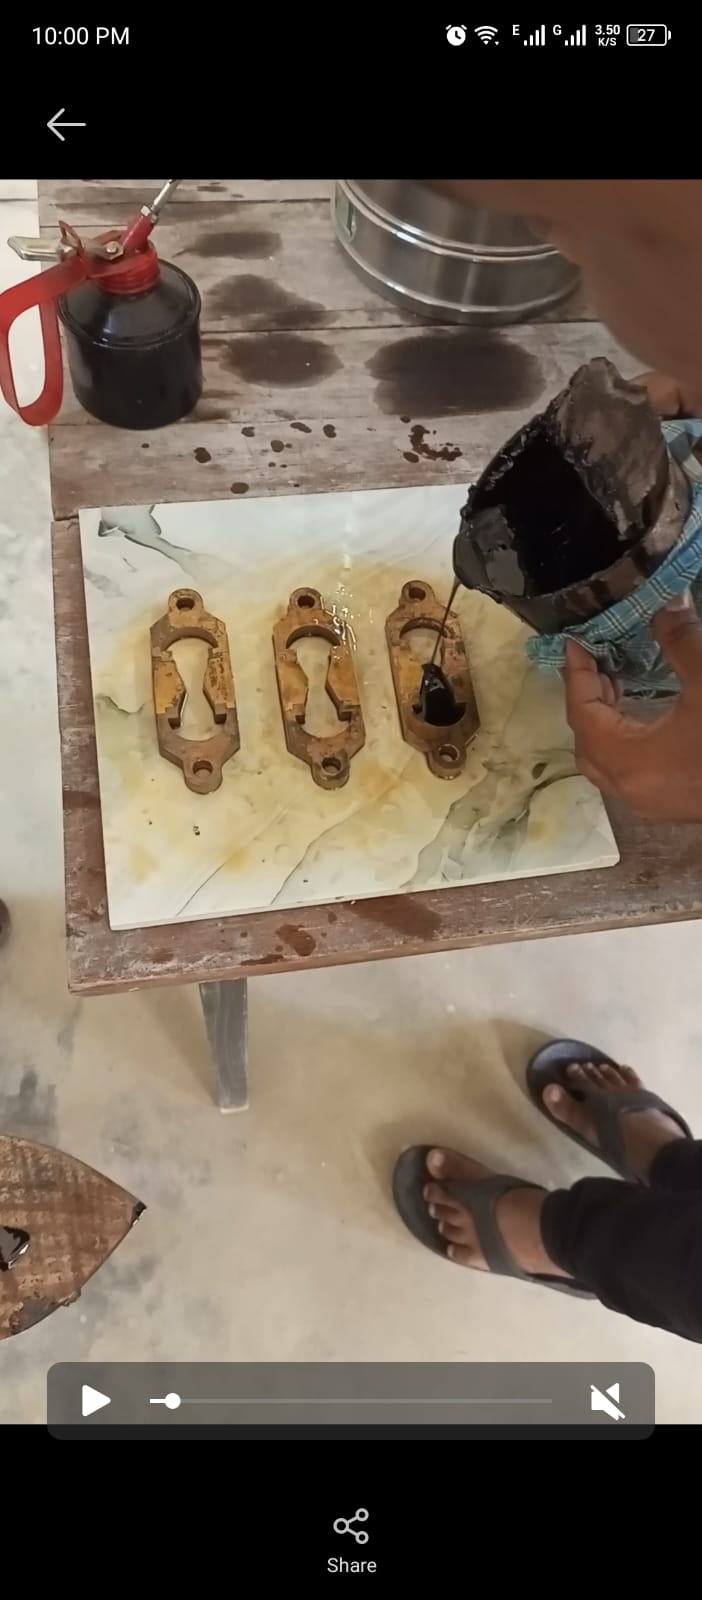
\includegraphics[width=4in, height=4in]{albums/appendix_04.jpeg}
\vspace{0.5cm}

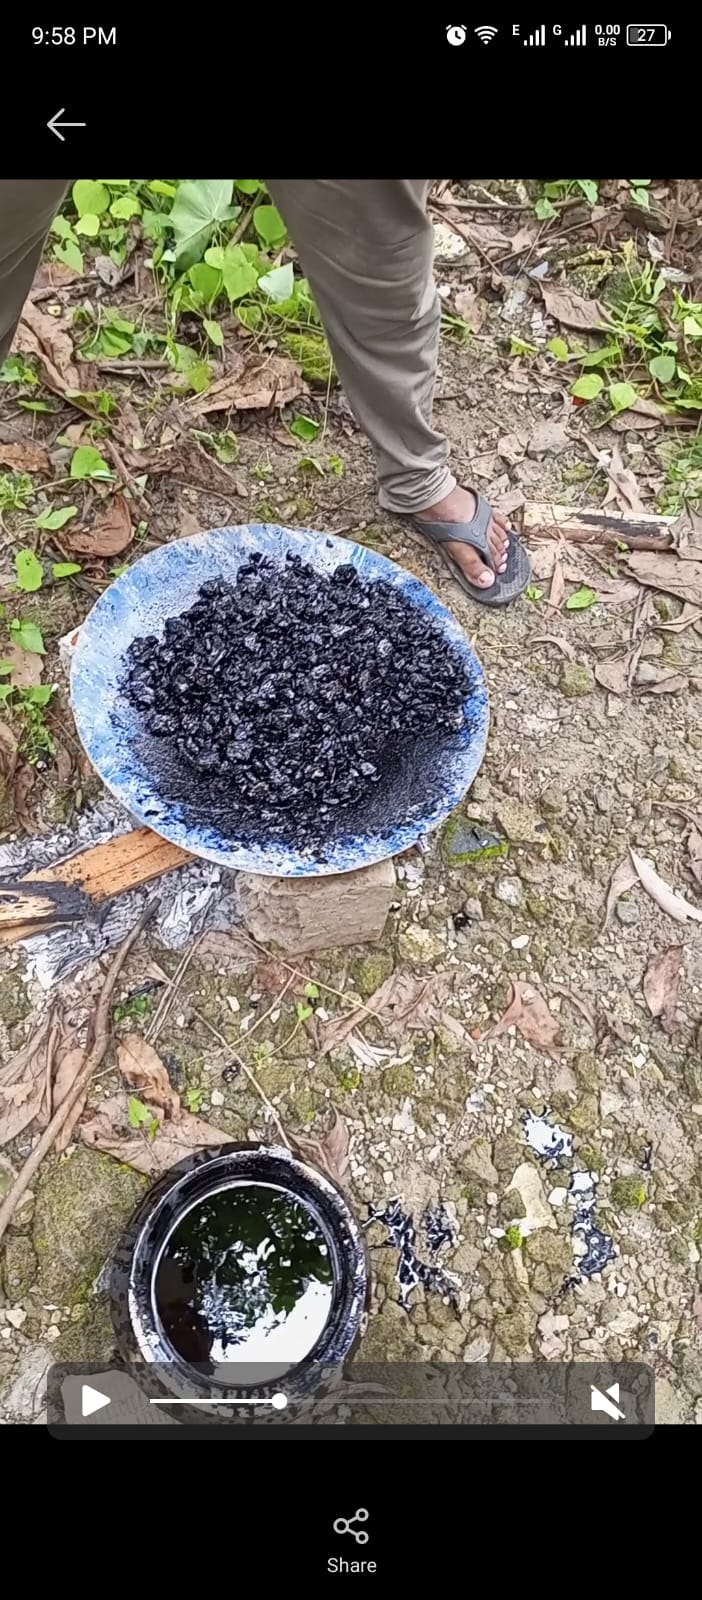
\includegraphics[width=4in, height=4in]{albums/appendix_05.jpeg}
\vspace{0.5cm}

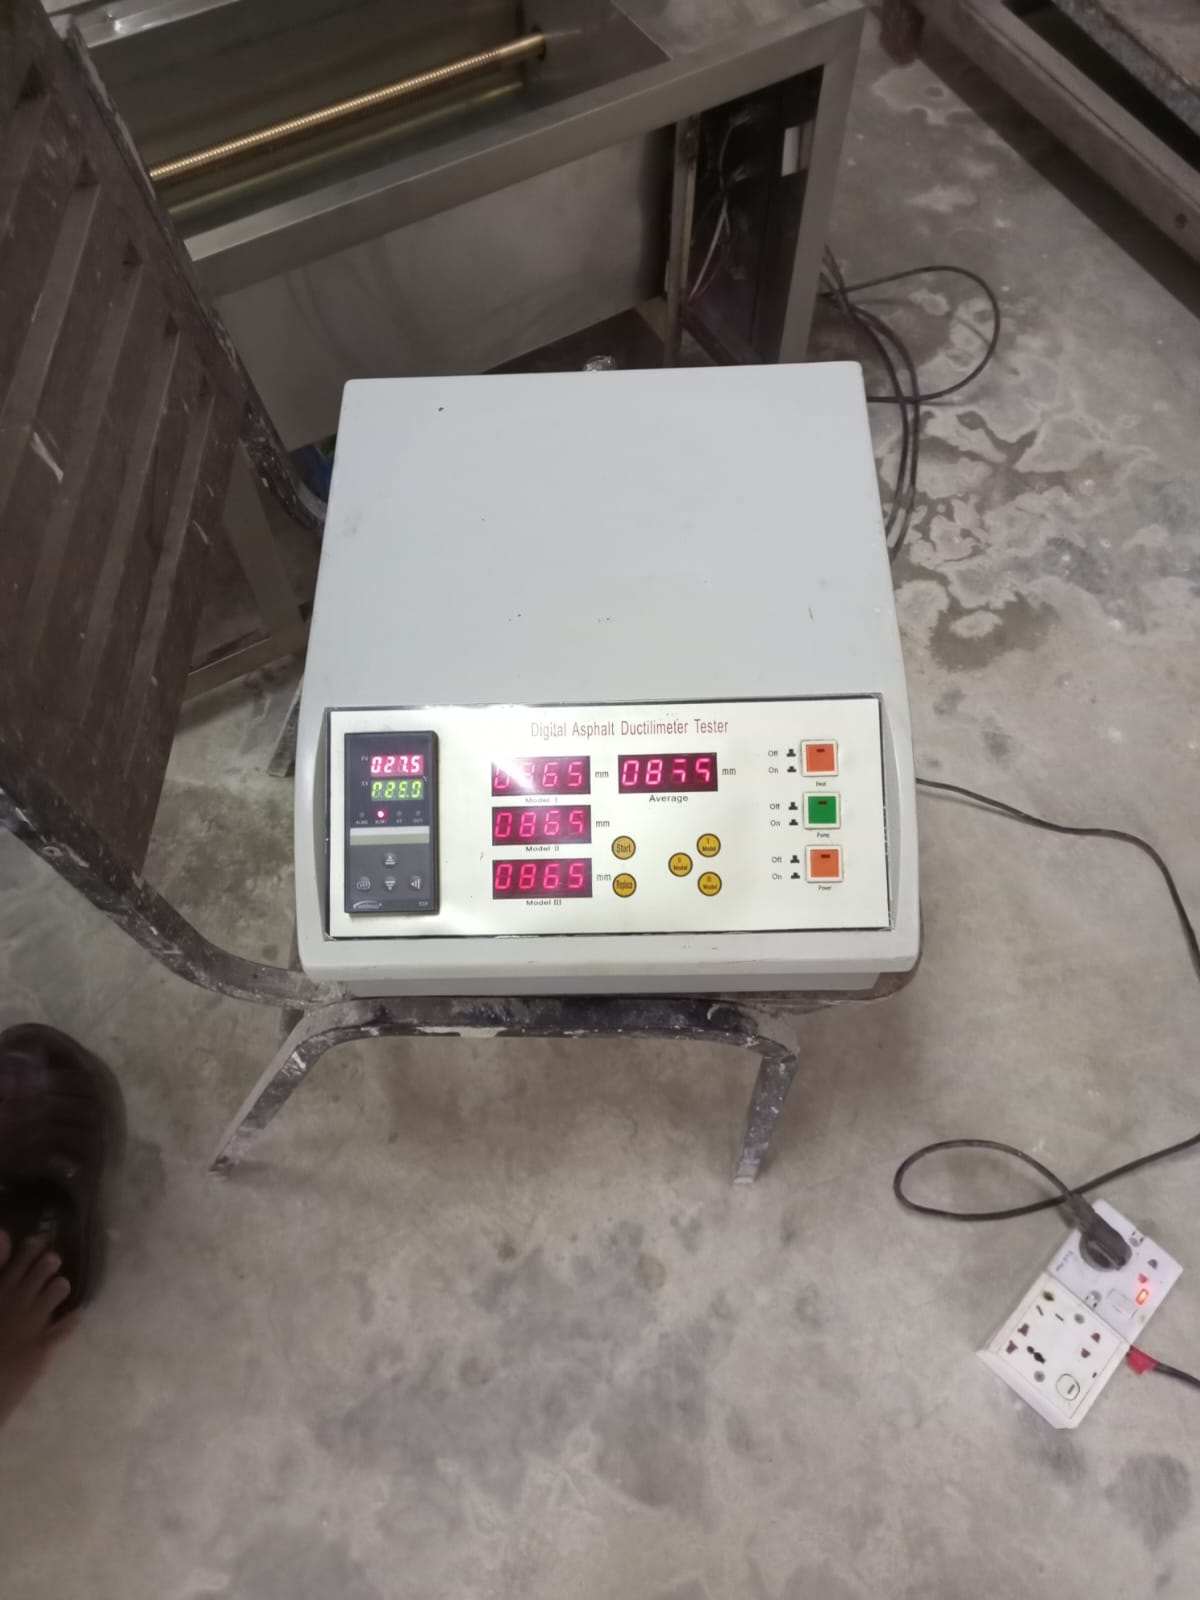
\includegraphics[width=4in, height=4in]{albums/appendix_06.jpeg}
\vspace{0.5cm}

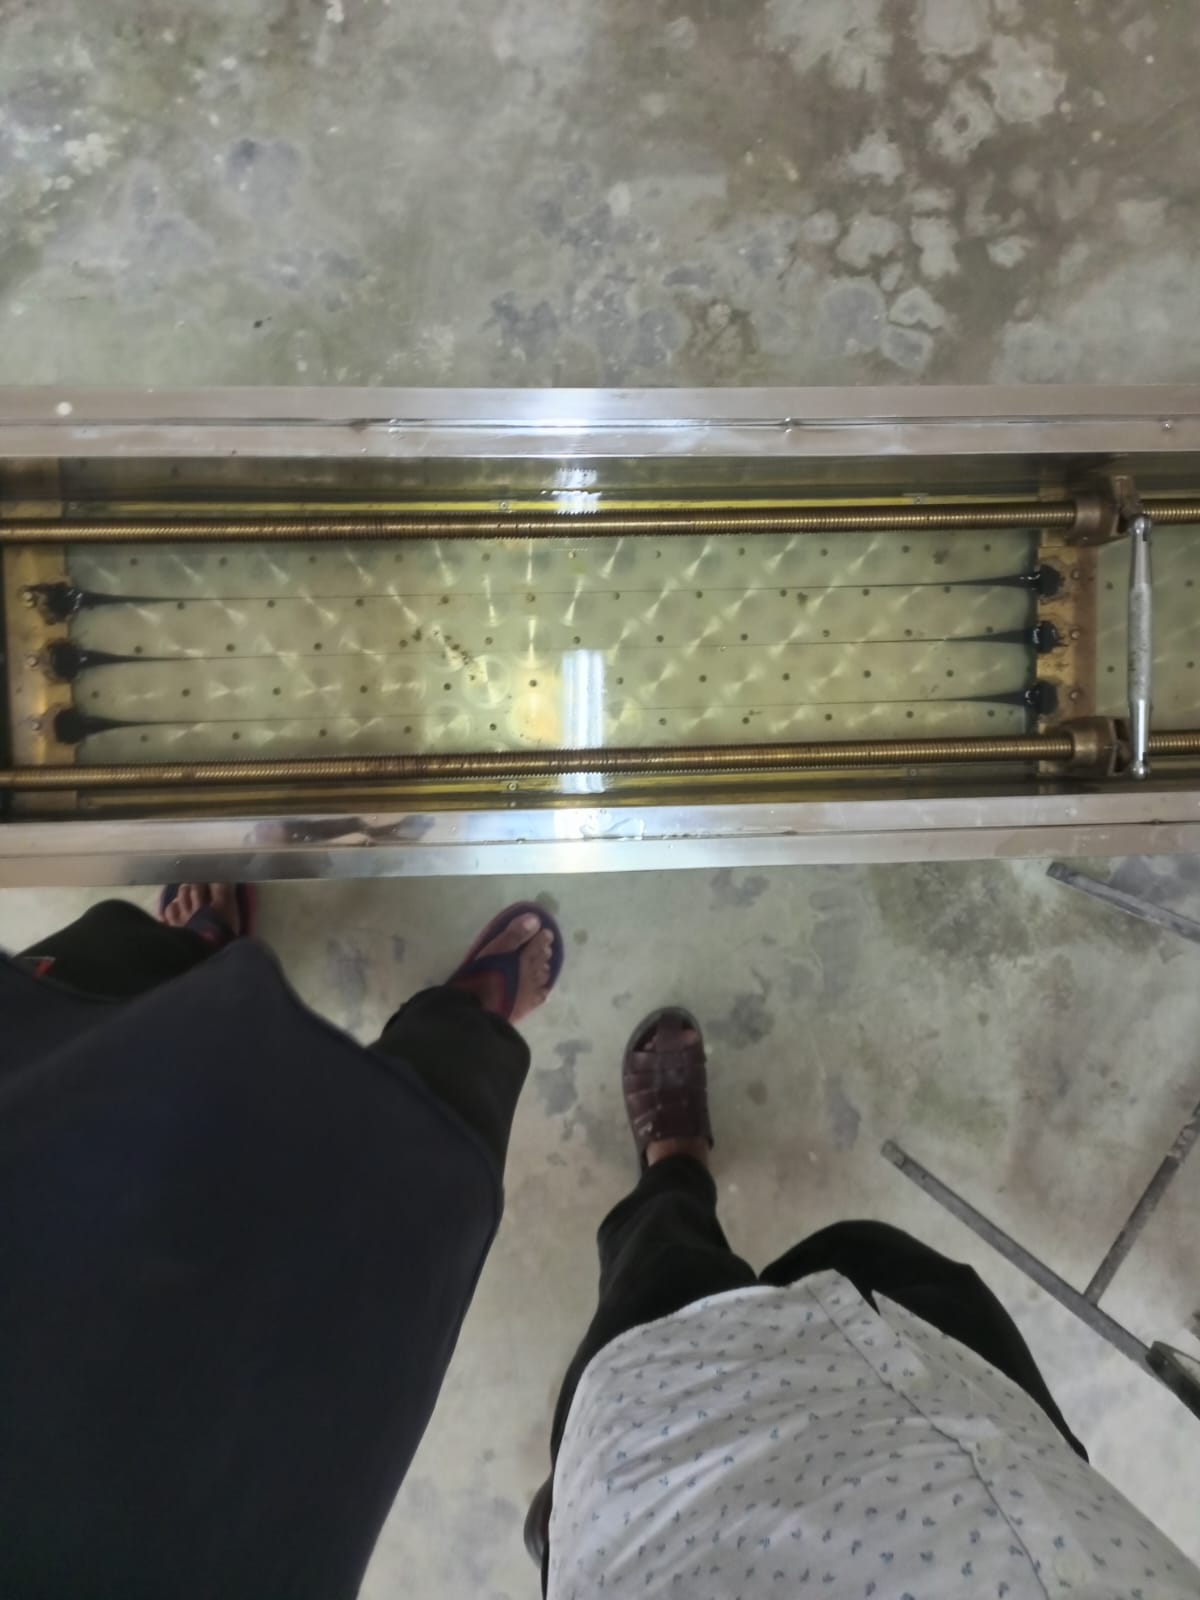
\includegraphics[width=4in, height=4in]{albums/appendix_07.jpeg}
\vspace{0.5cm}

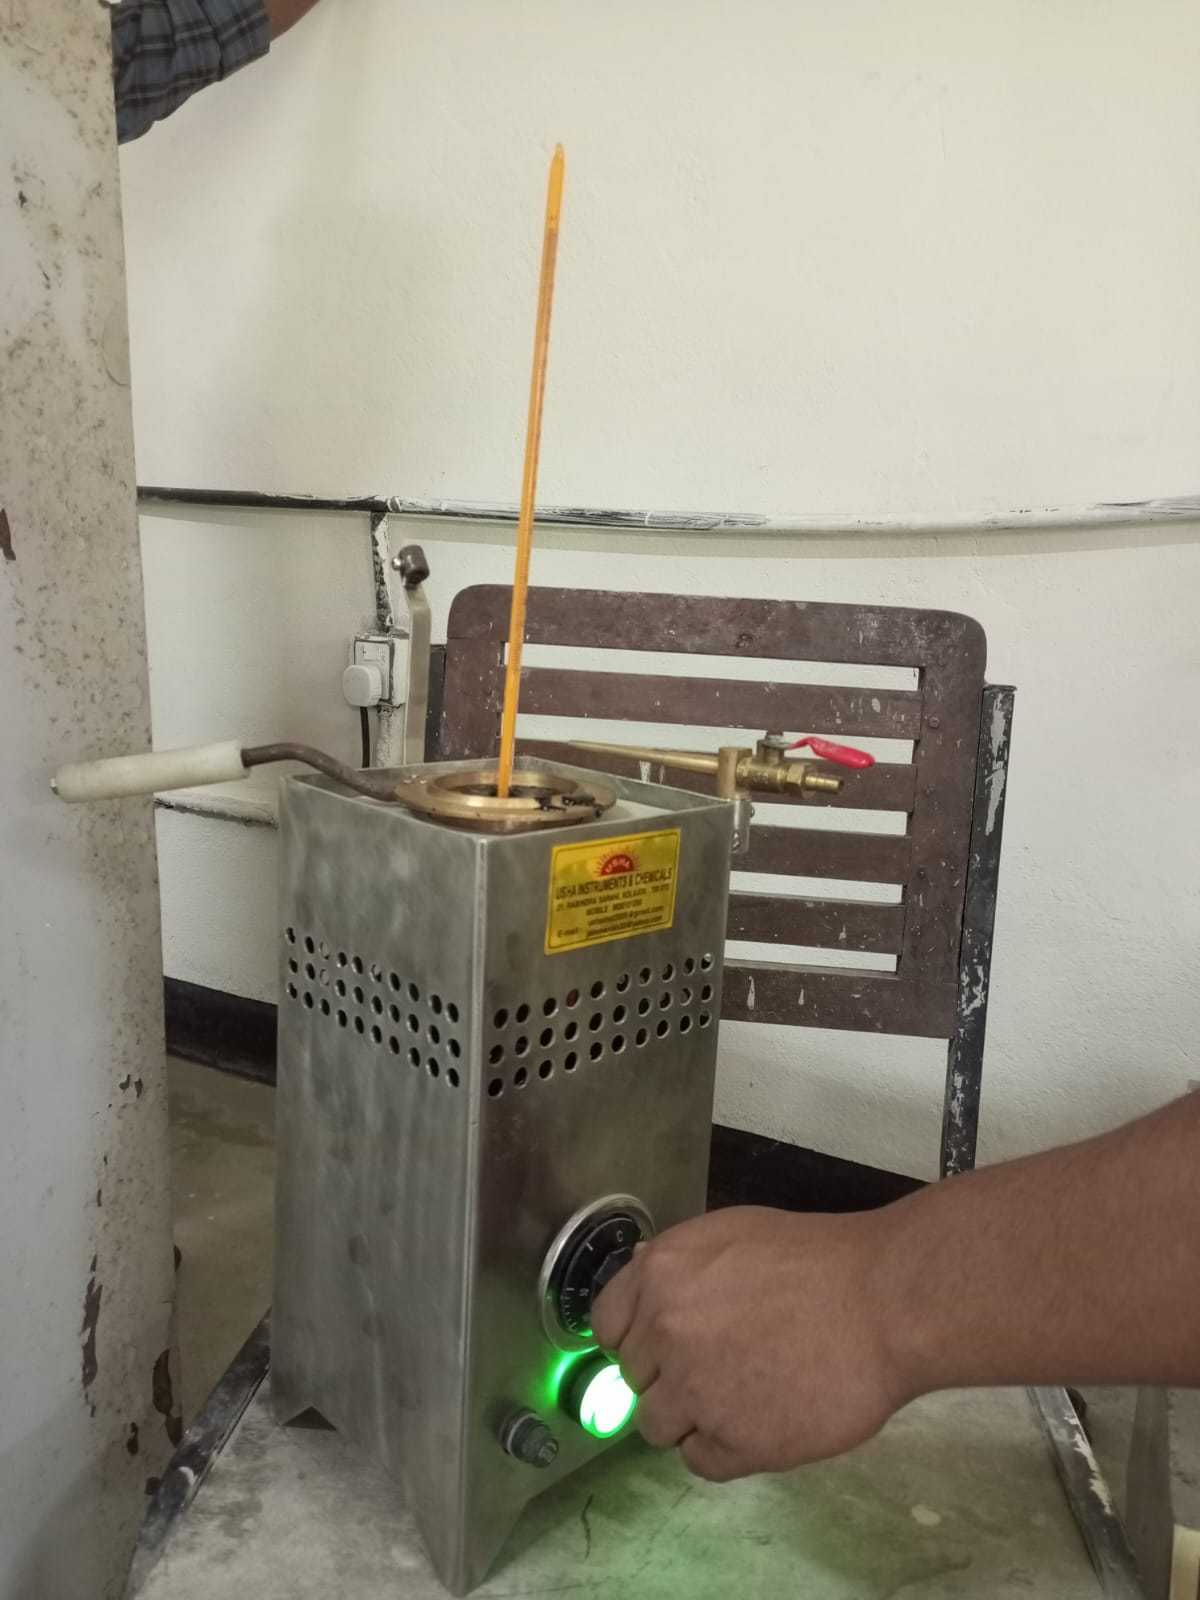
\includegraphics[width=4in, height=4in]{albums/appendix_08.jpeg}
\vspace{0.5cm}

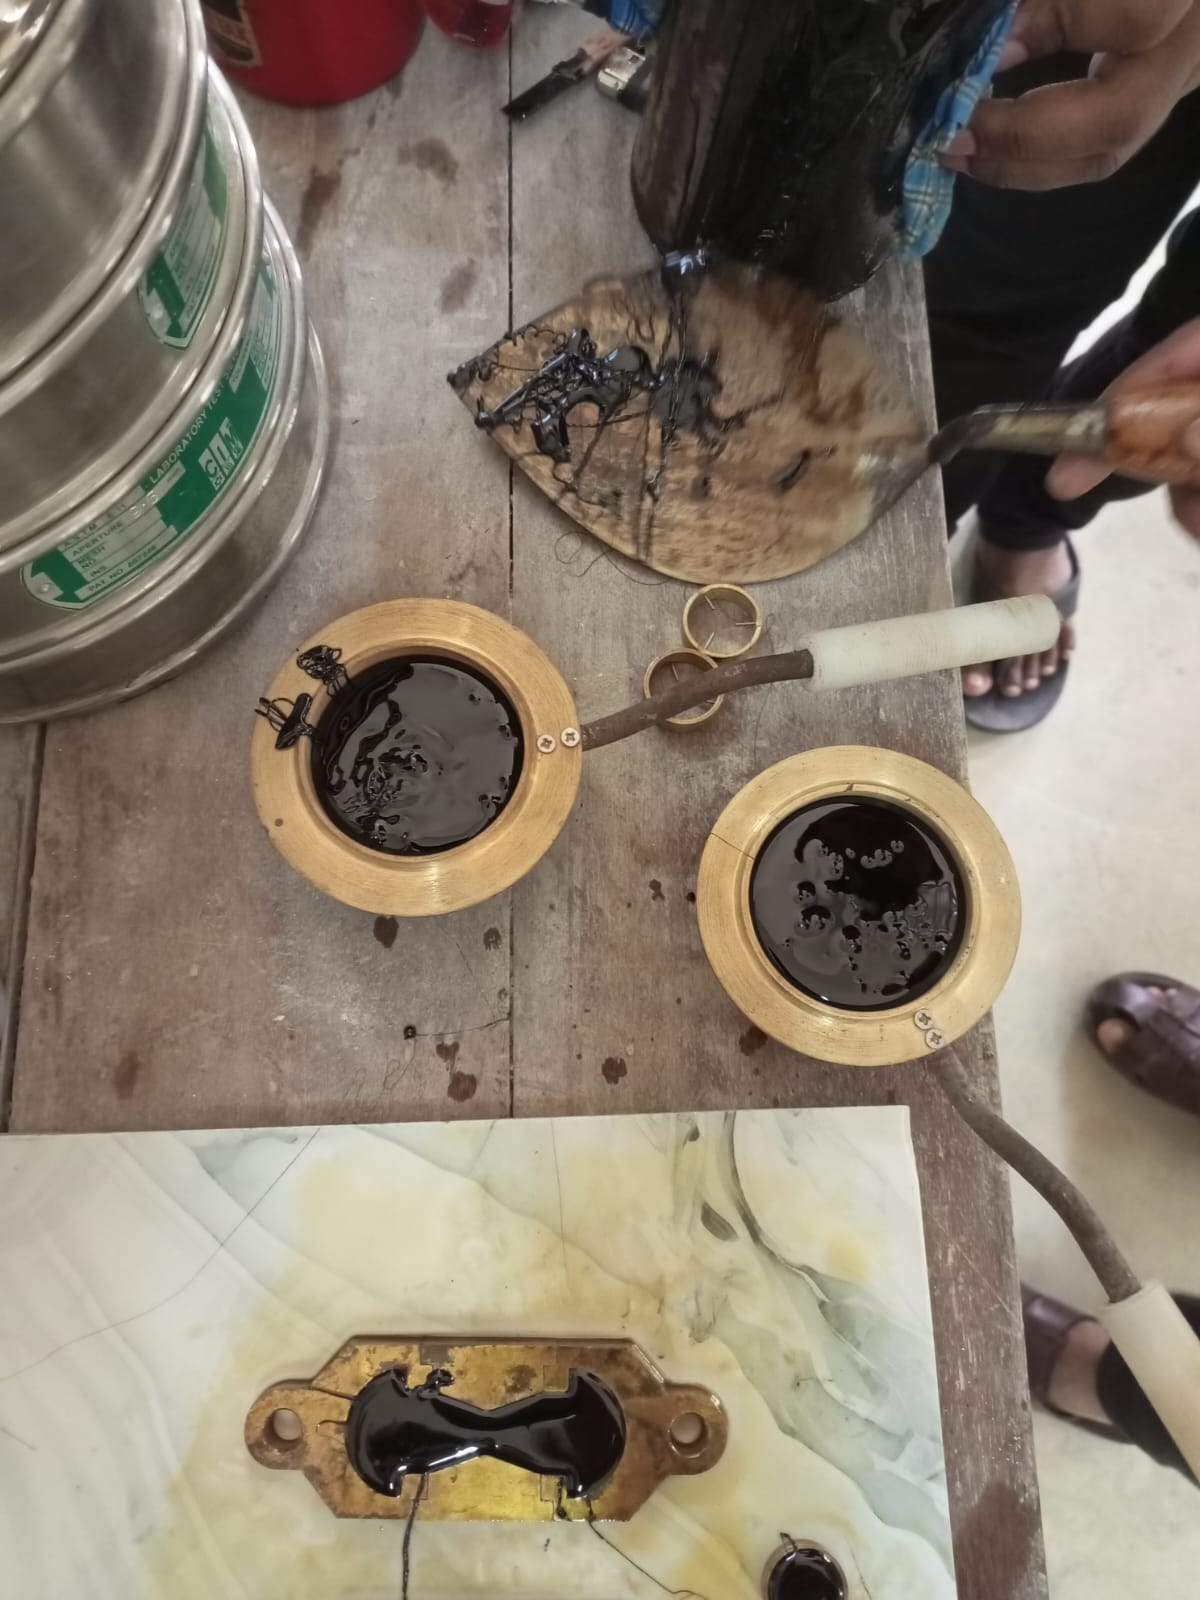
\includegraphics[width=4in, height=4in]{albums/appendix_09.jpeg}
\vspace{0.5cm}

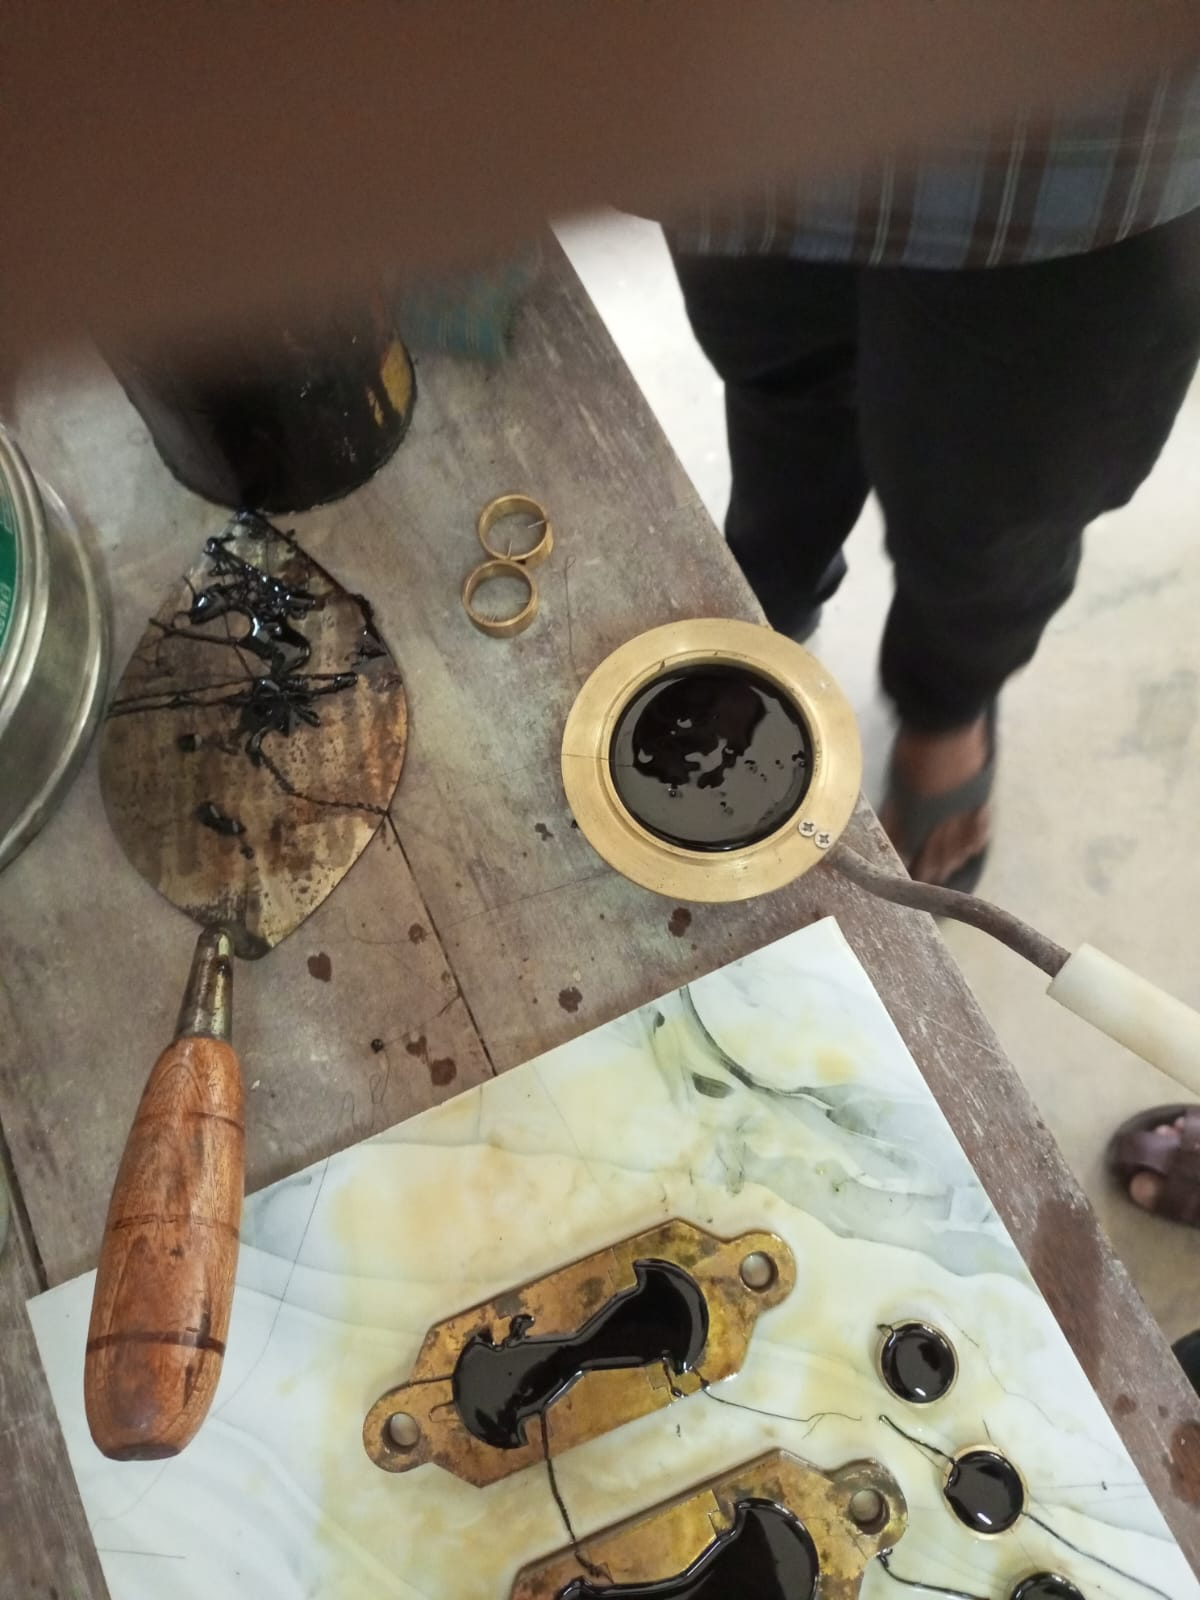
\includegraphics[width=4in, height=4in]{albums/appendix_10.jpeg}
\vspace{0.5cm}

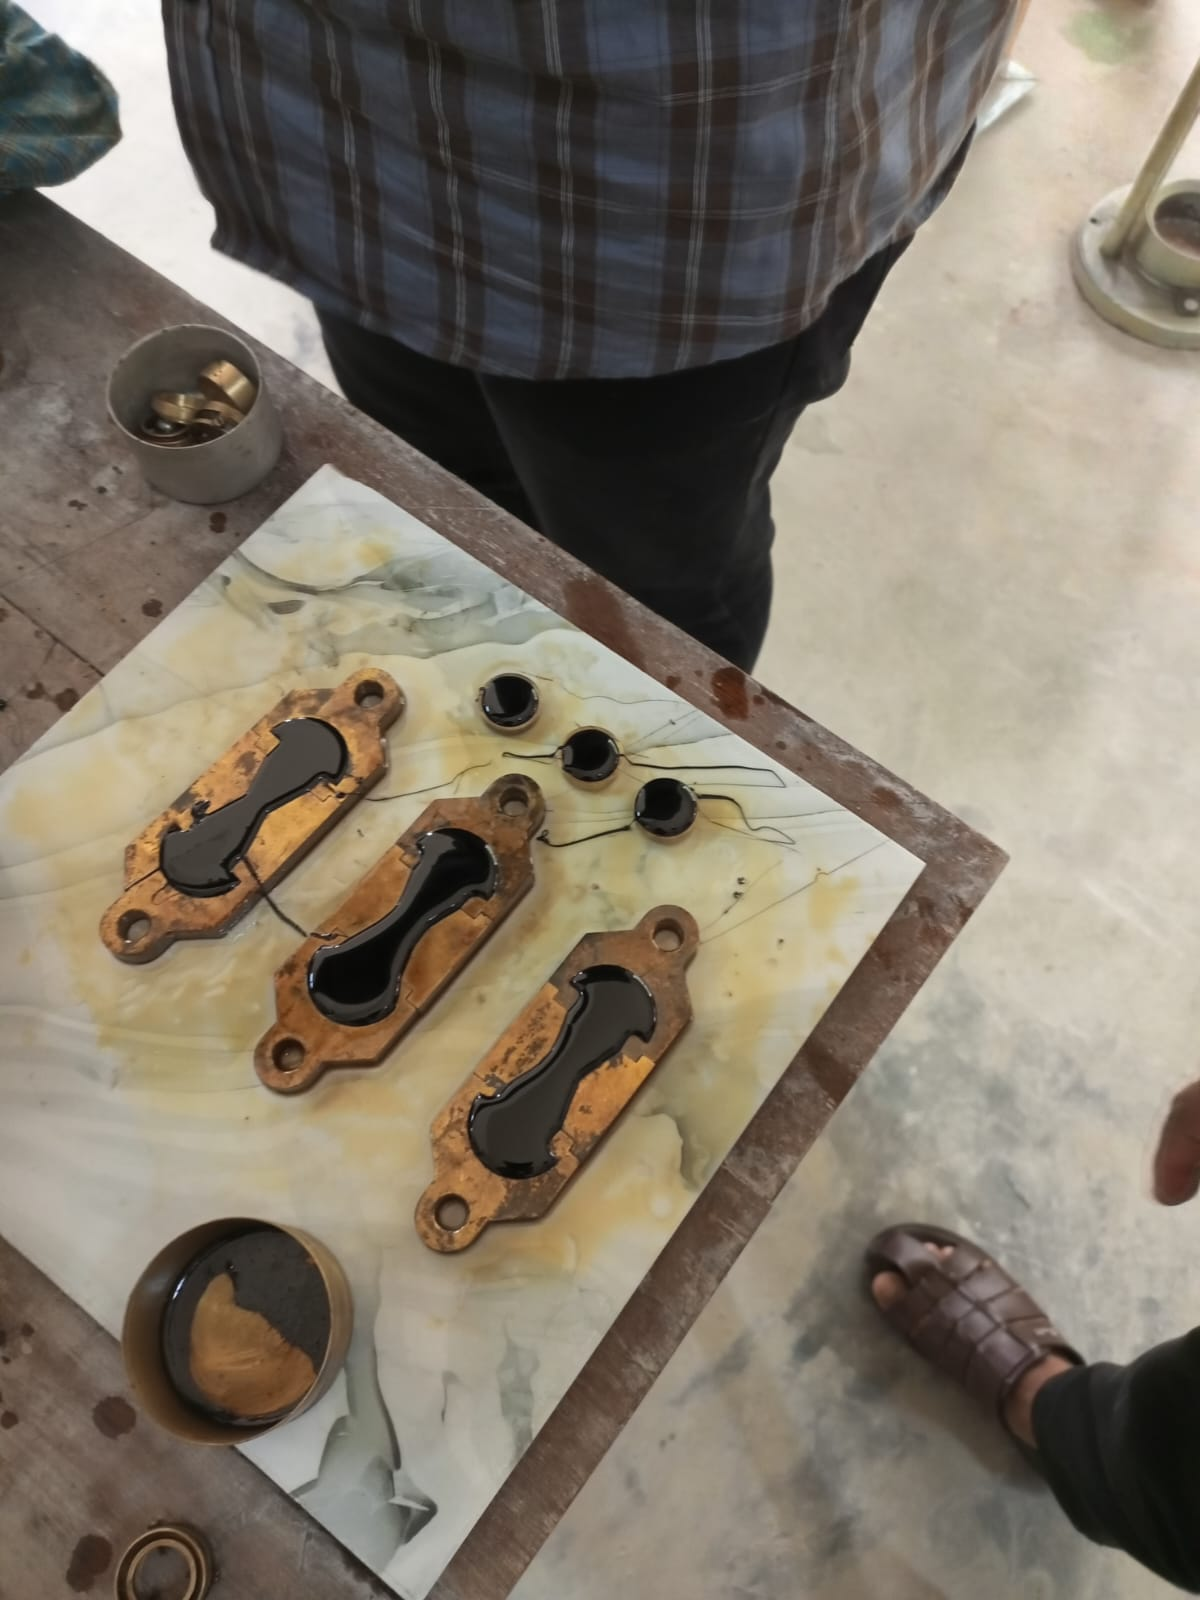
\includegraphics[width=4in, height=4in]{albums/appendix_11.jpeg}
\vspace{0.5cm}

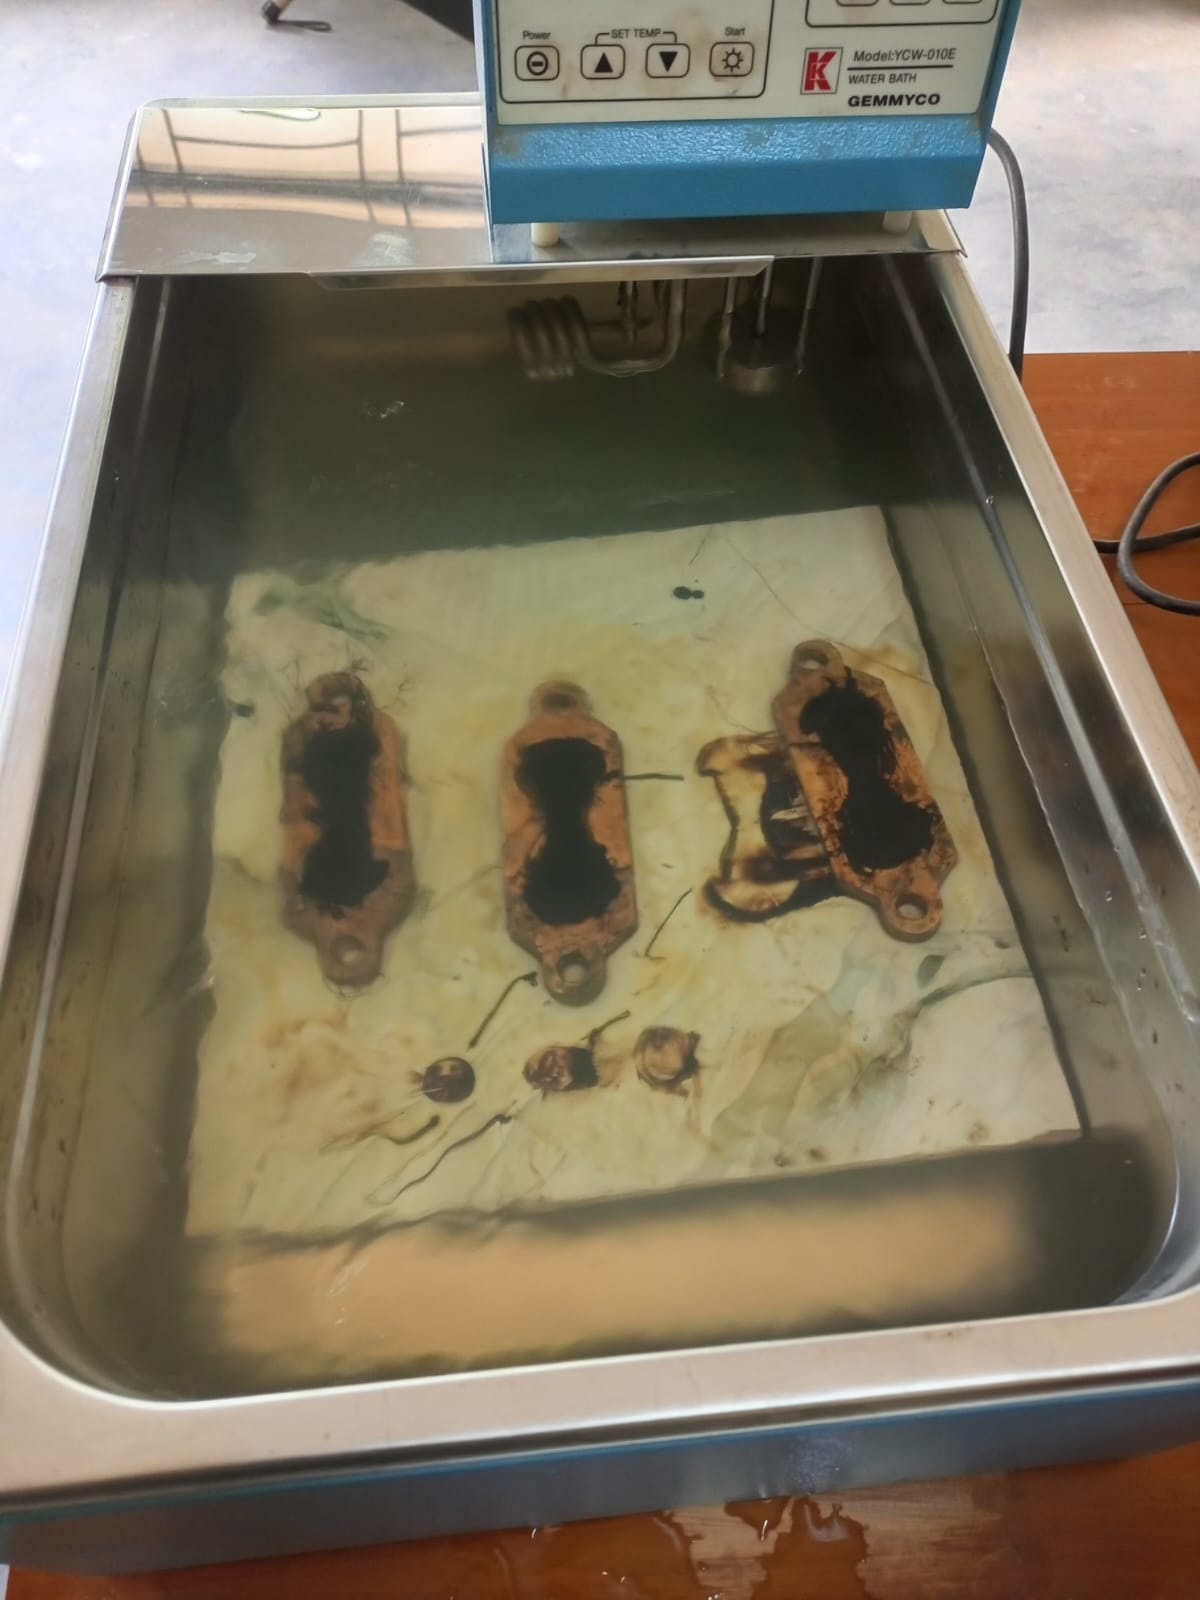
\includegraphics[width=4in, height=4in]{albums/appendix_12.jpeg}
\vspace{0.5cm}

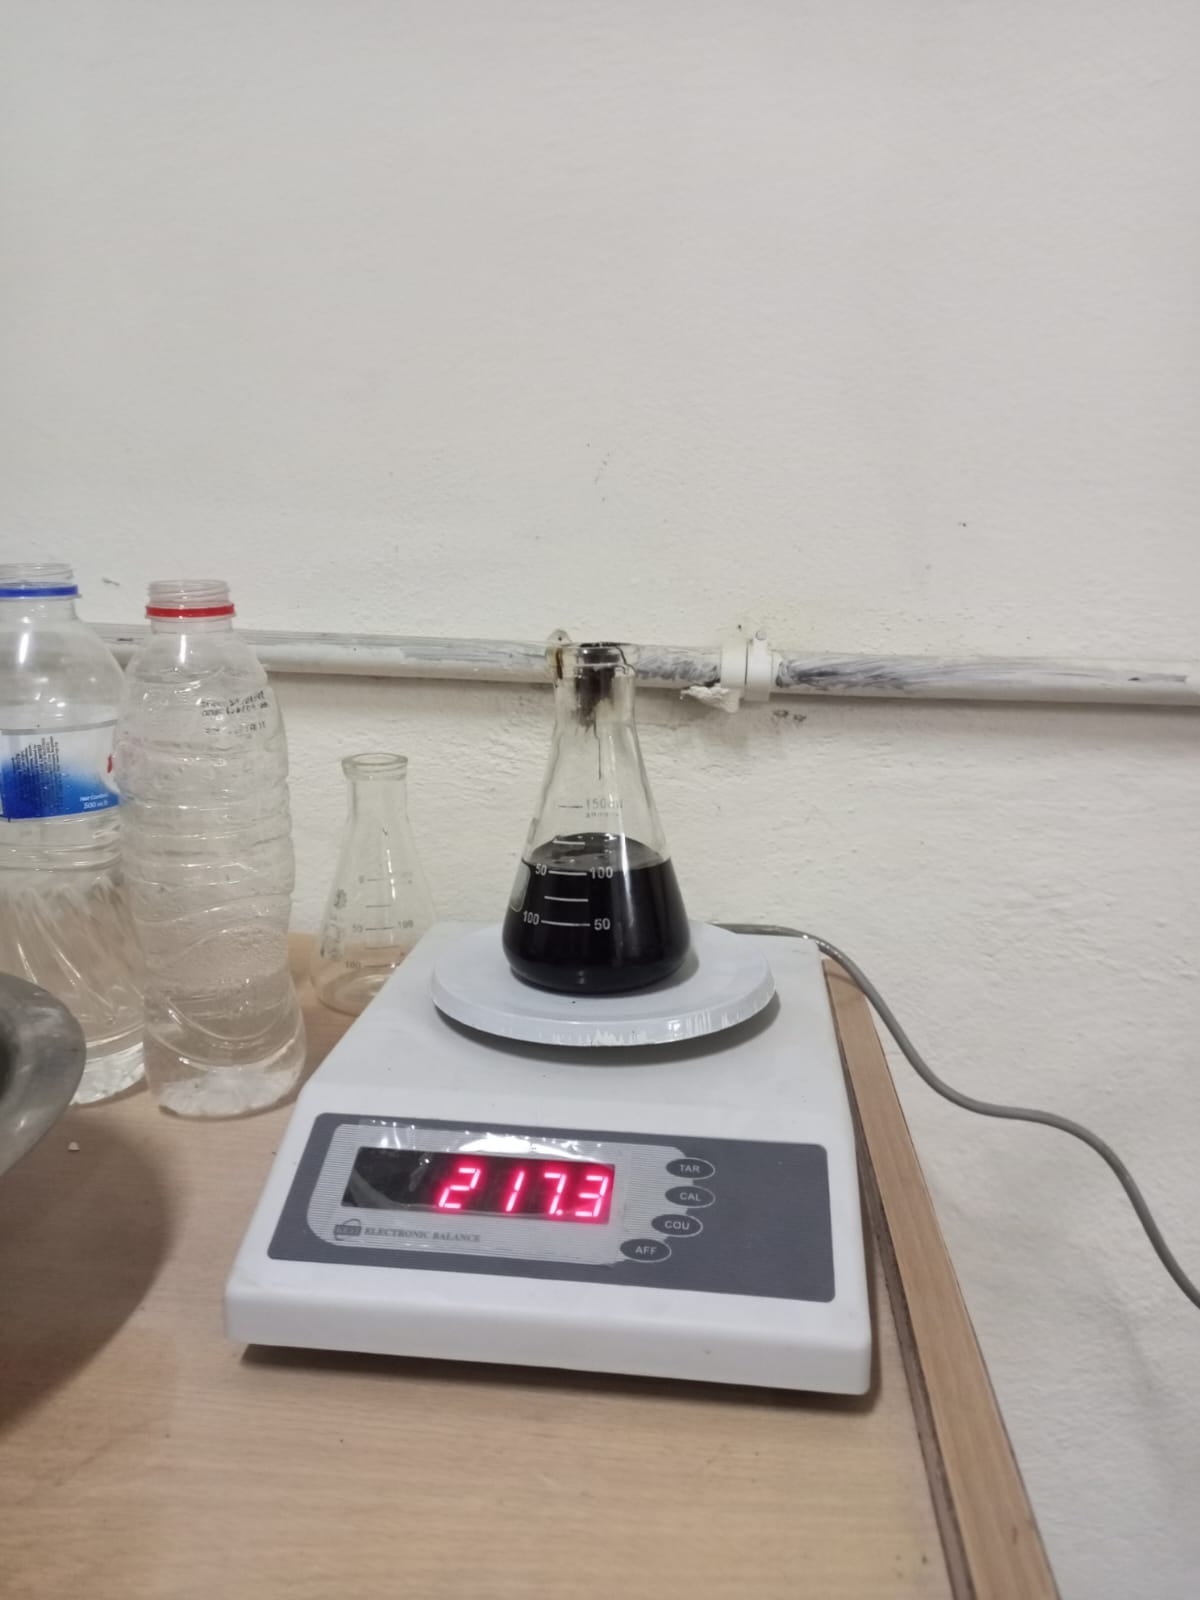
\includegraphics[width=4in, height=4in]{albums/appendix_13.jpeg}
\vspace{0.5cm}

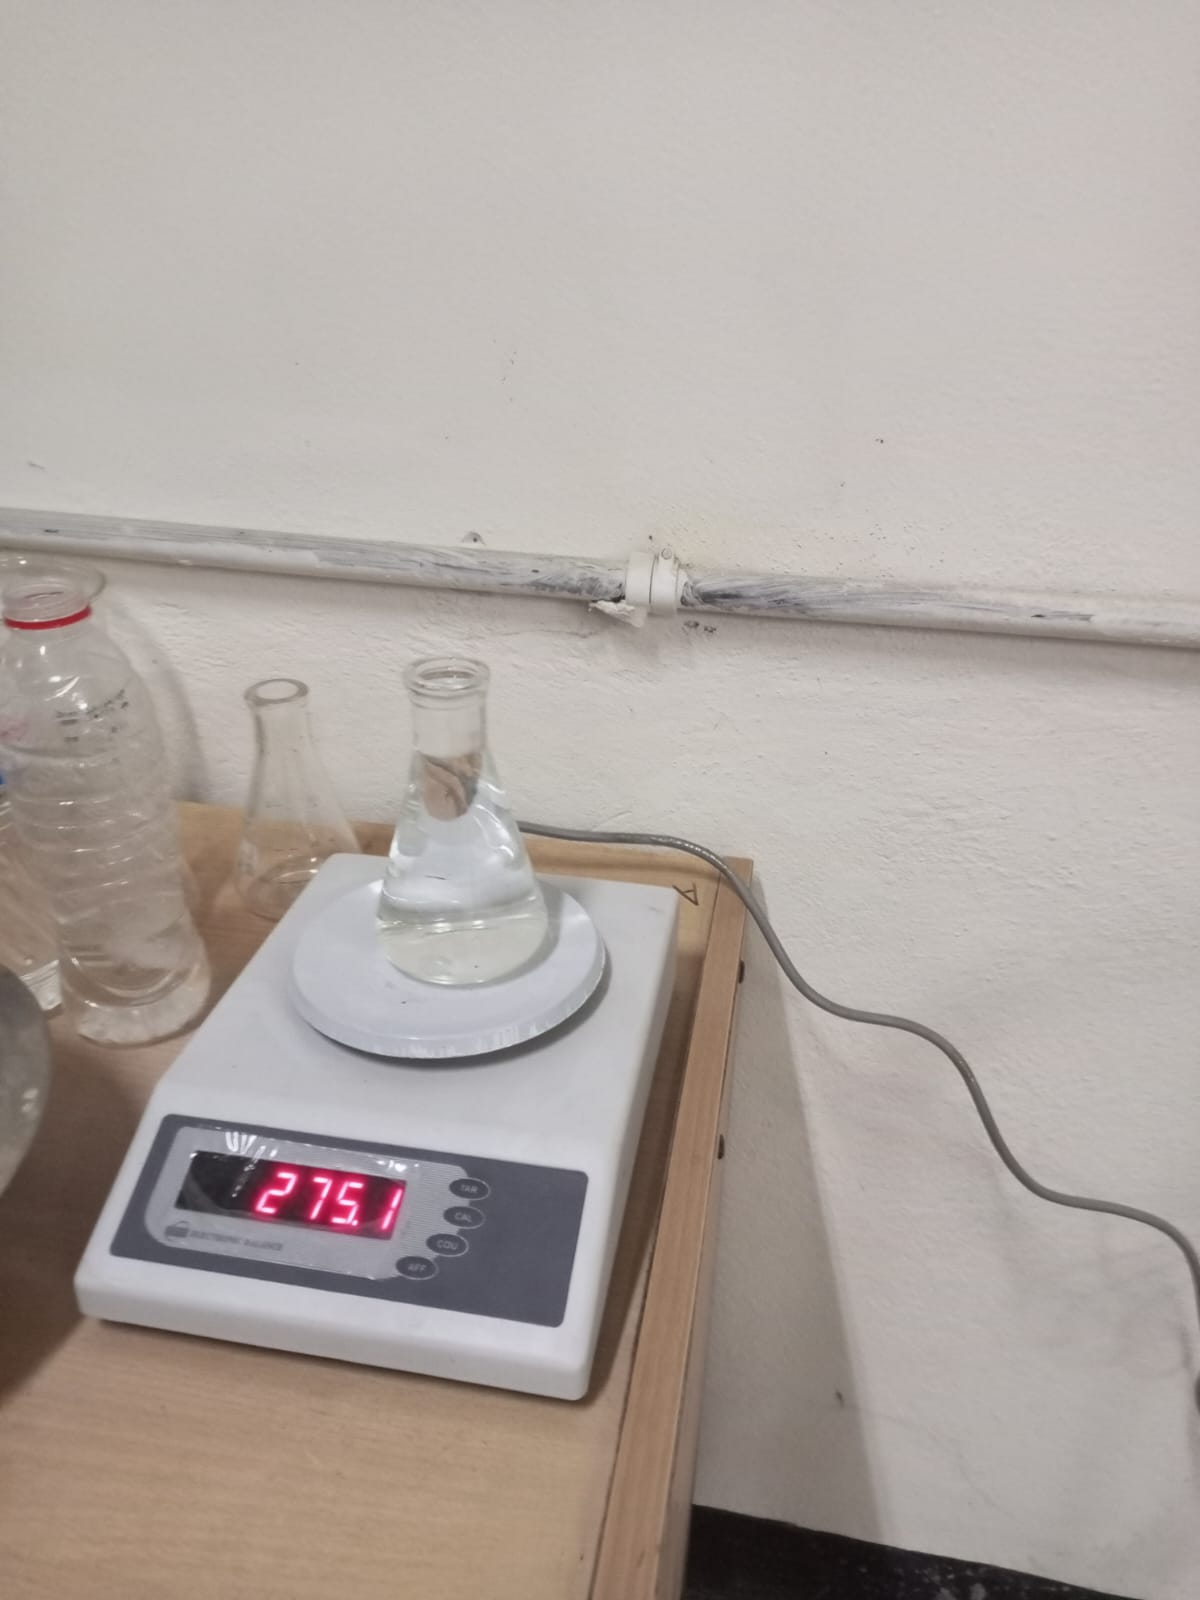
\includegraphics[width=4in, height=4in]{albums/appendix_14.jpeg}
\vspace{0.5cm}

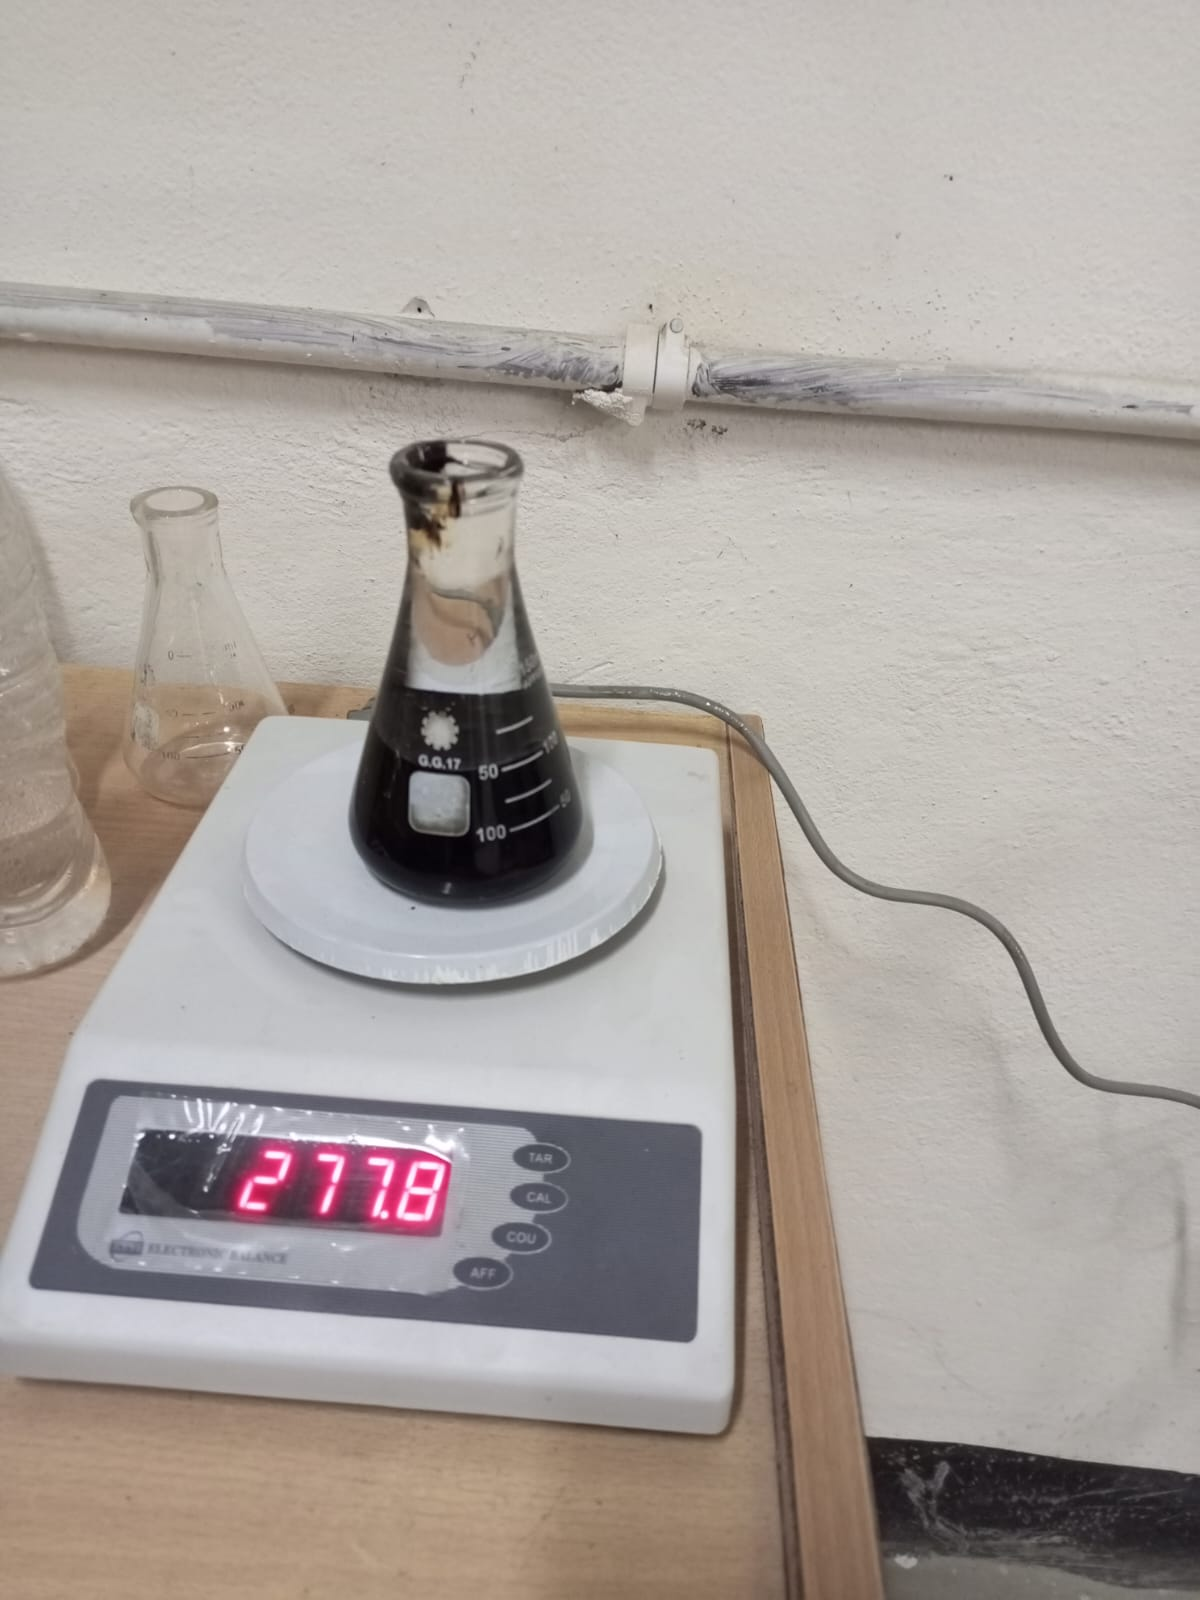
\includegraphics[width=4in, height=4in]{albums/appendix_15.jpeg}
\vspace{0.5cm}

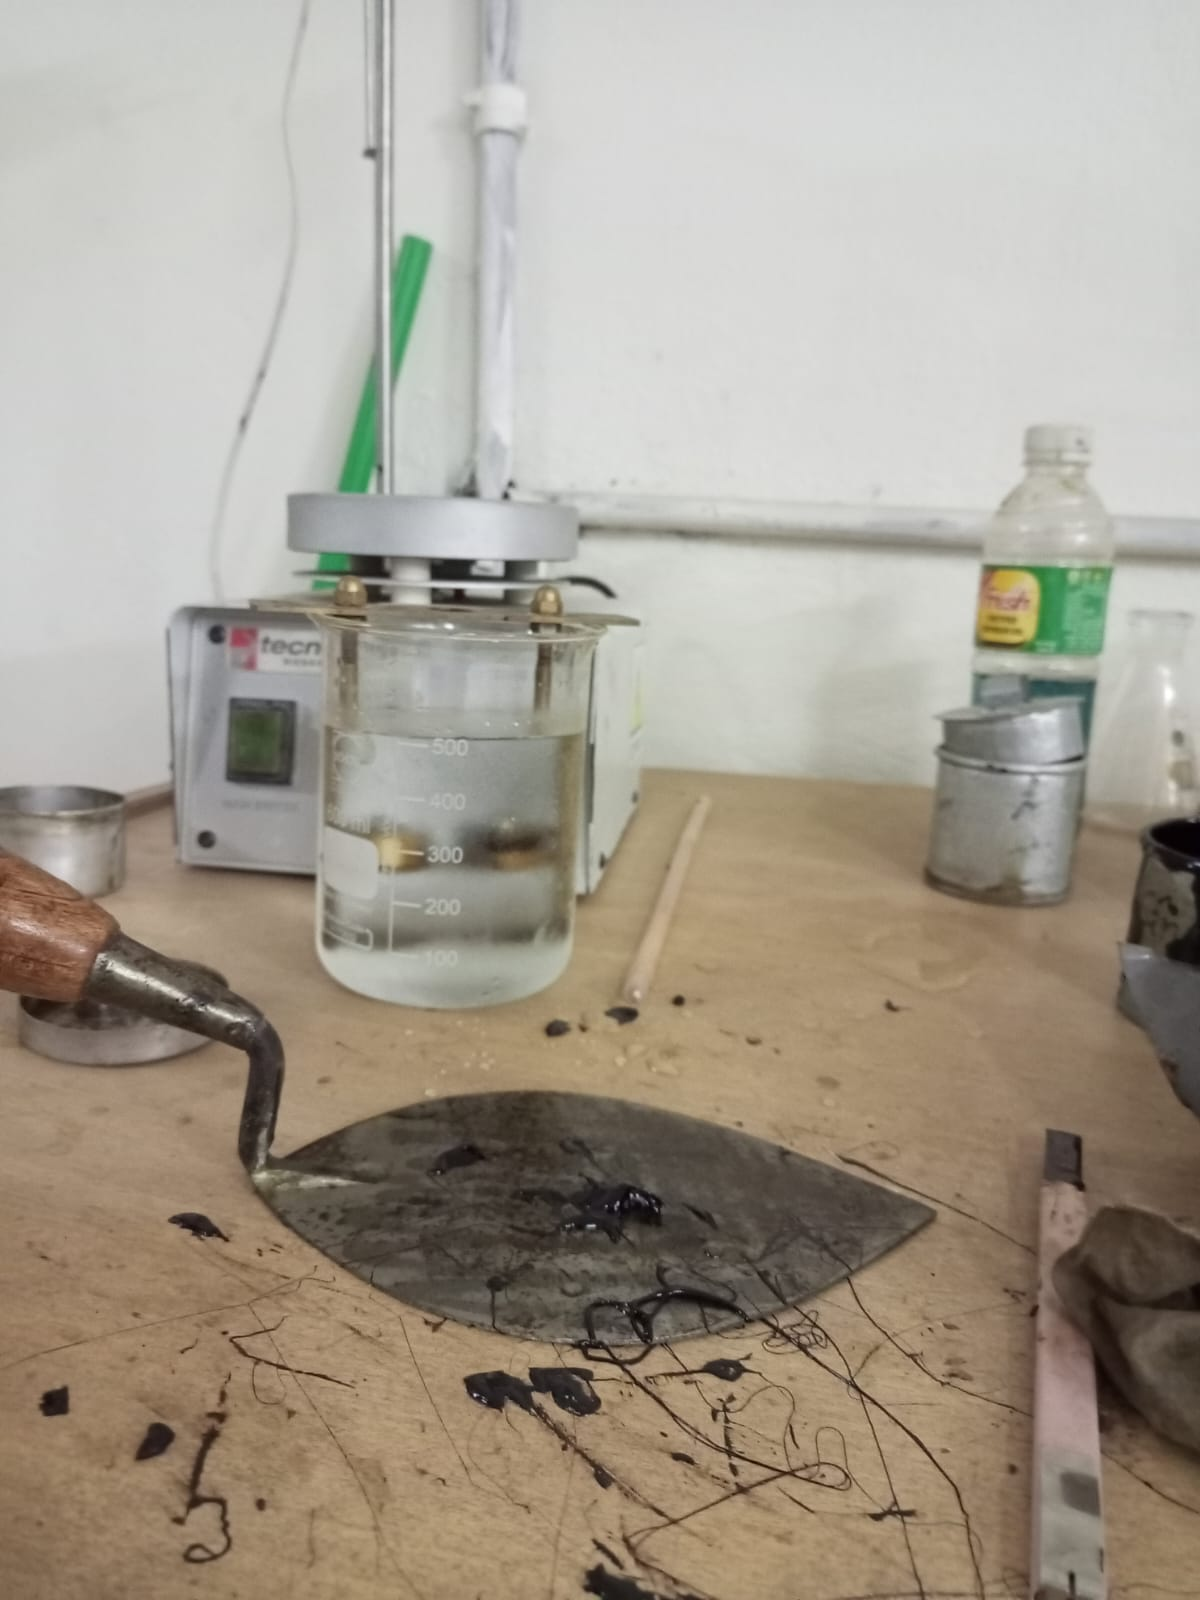
\includegraphics[width=4in, height=4in]{albums/appendix_16.jpeg}
\vspace{0.5cm}

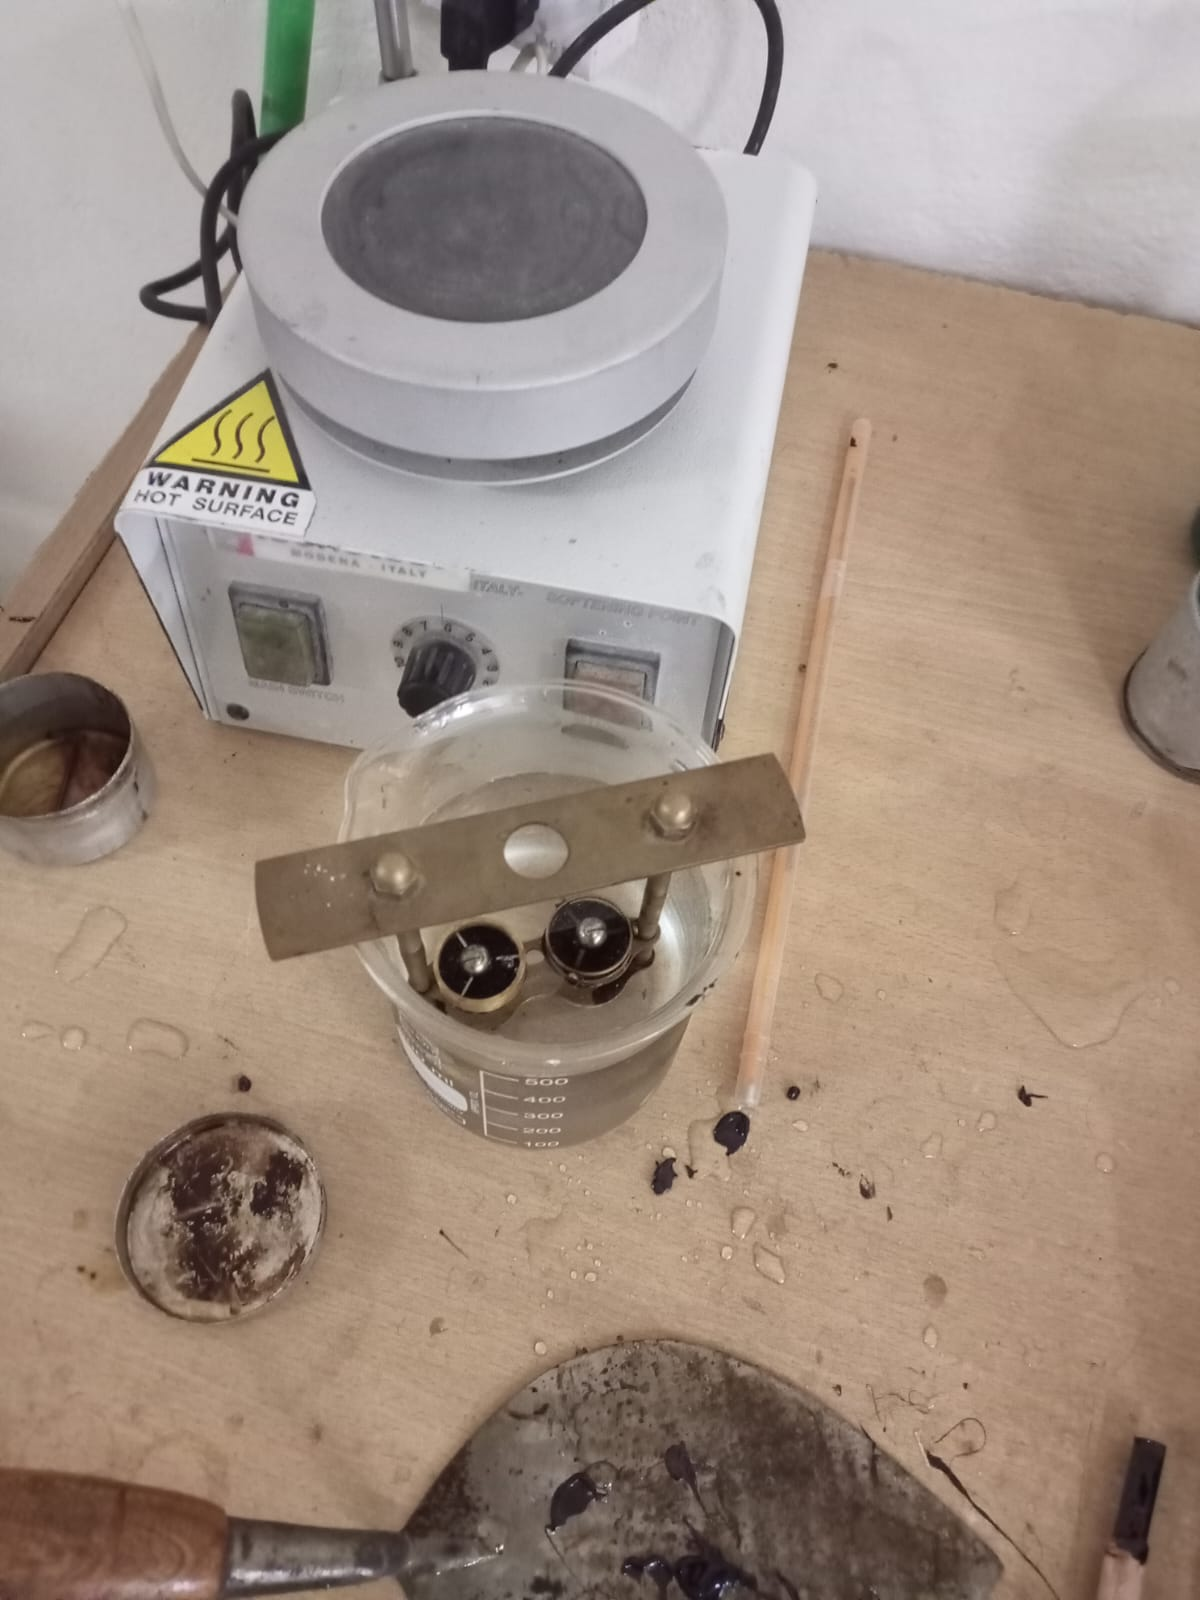
\includegraphics[width=4in, height=4in]{albums/appendix_17.jpeg}
\vspace{0.5cm}

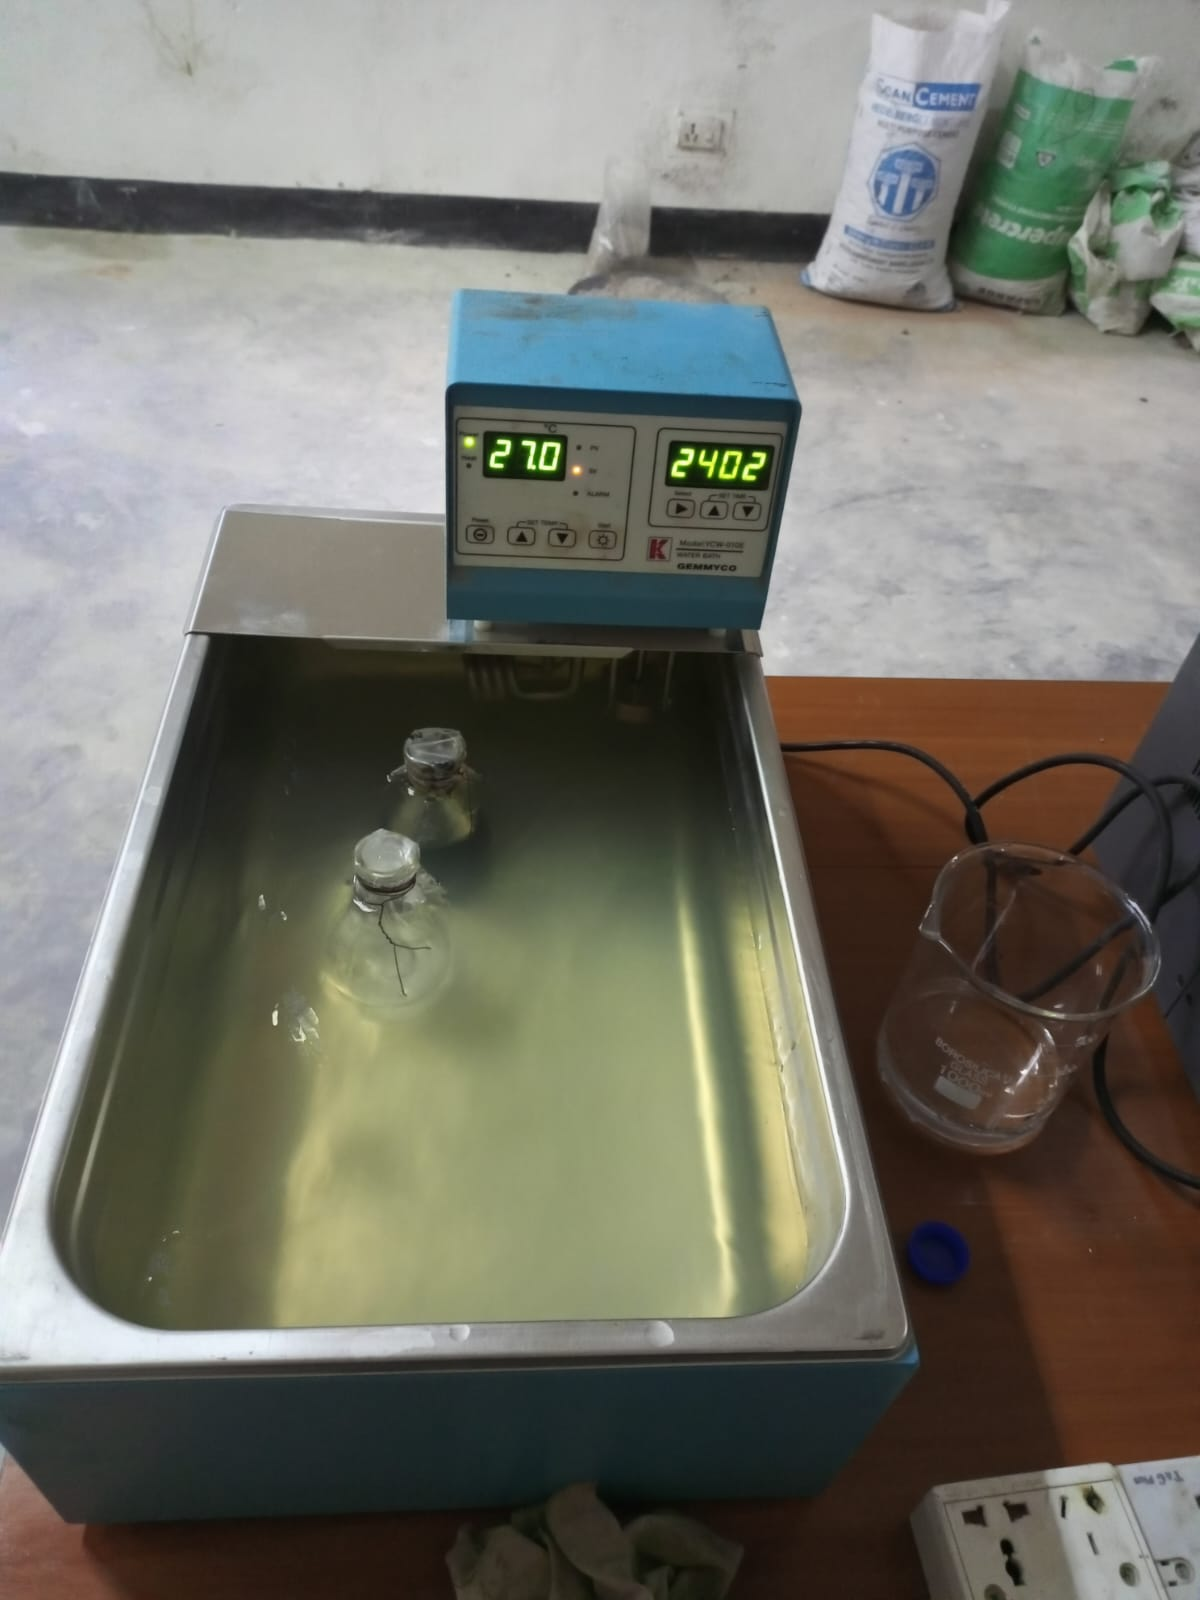
\includegraphics[width=4in, height=4in]{albums/appendix_18.jpeg}
\vspace{0.5cm}

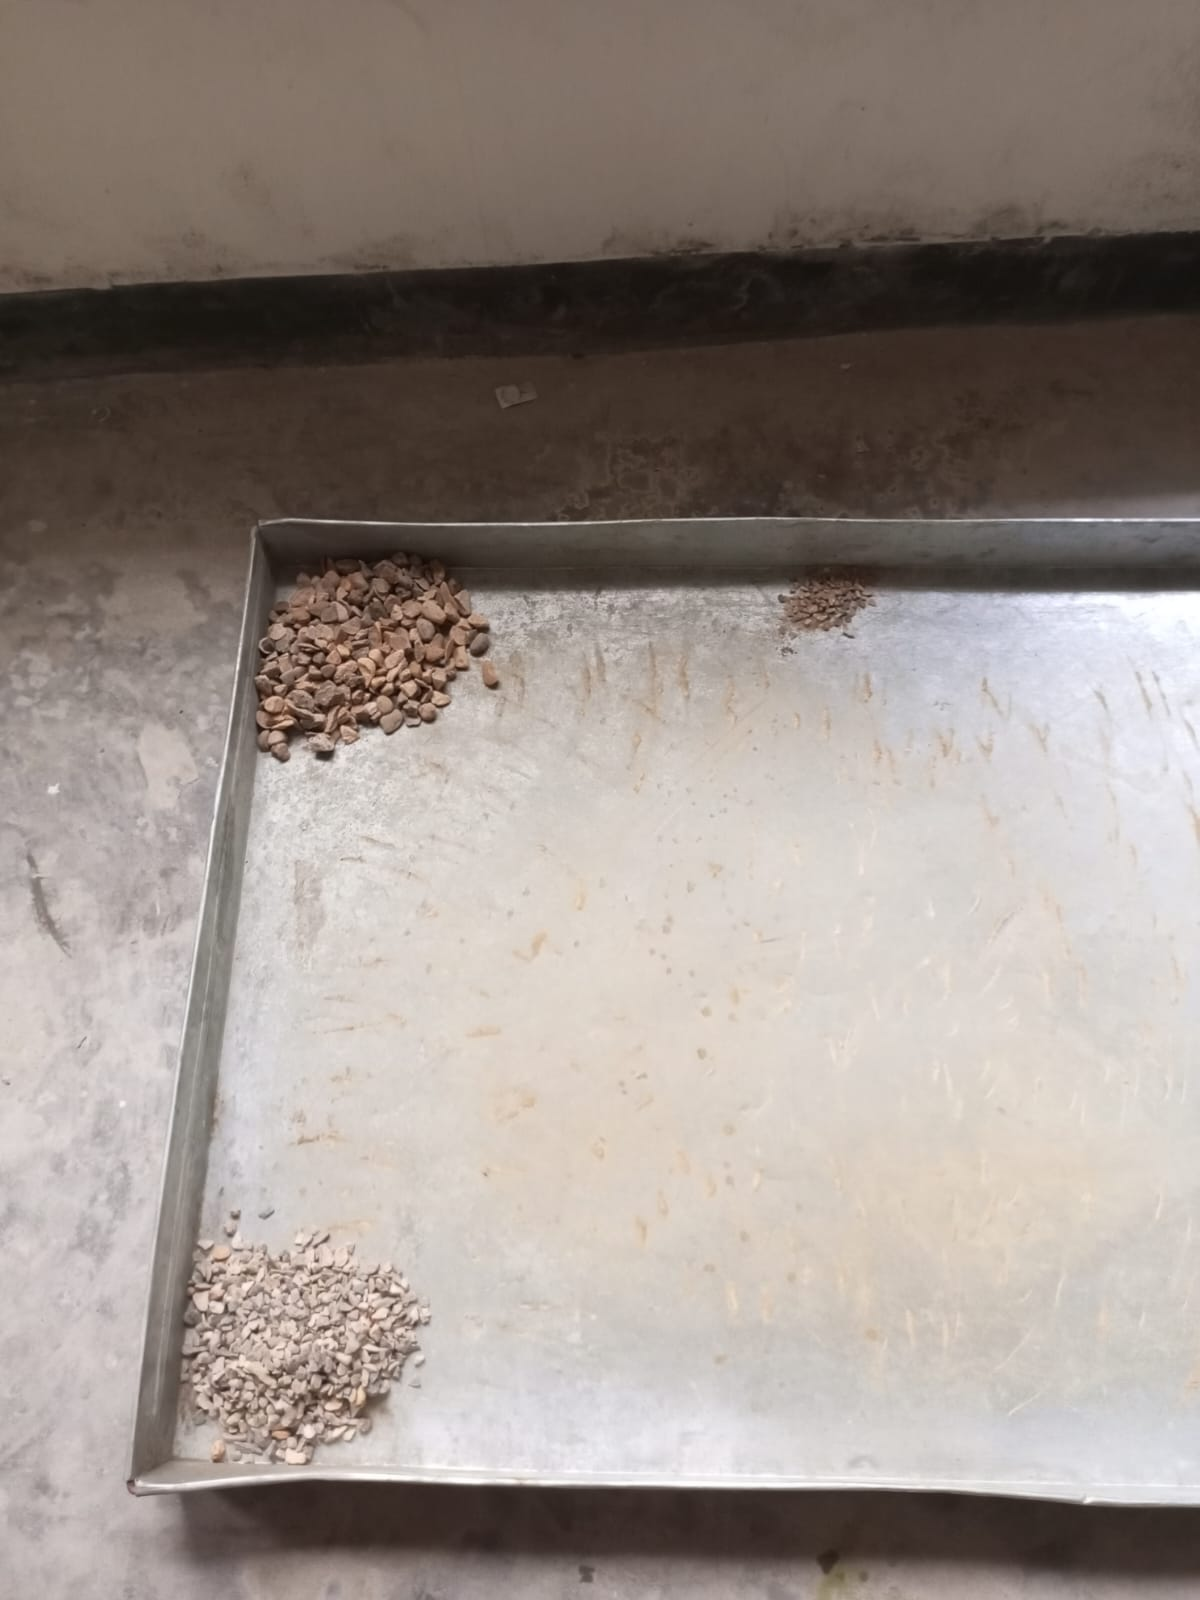
\includegraphics[width=4in, height=4in]{albums/appendix_19.jpeg}
\vspace{0.5cm}

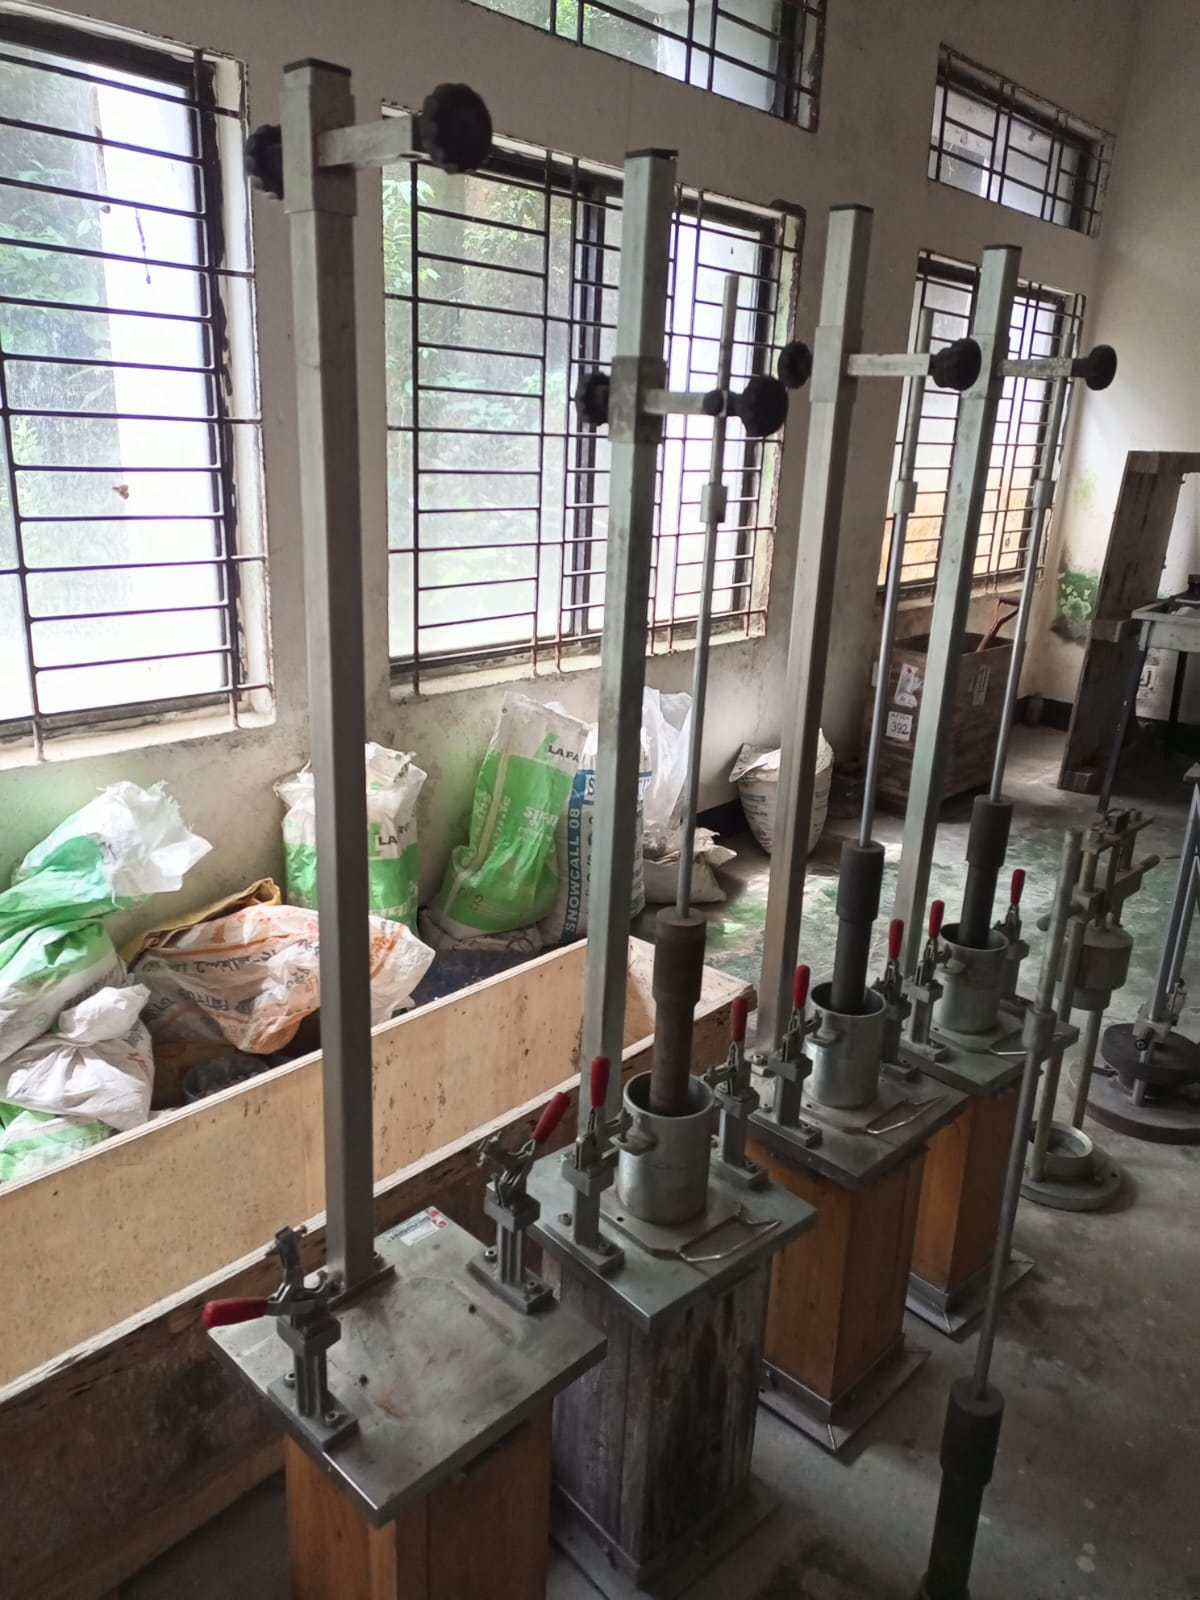
\includegraphics[width=4in, height=4in]{albums/appendix_20.jpeg}
\vspace{0.5cm}

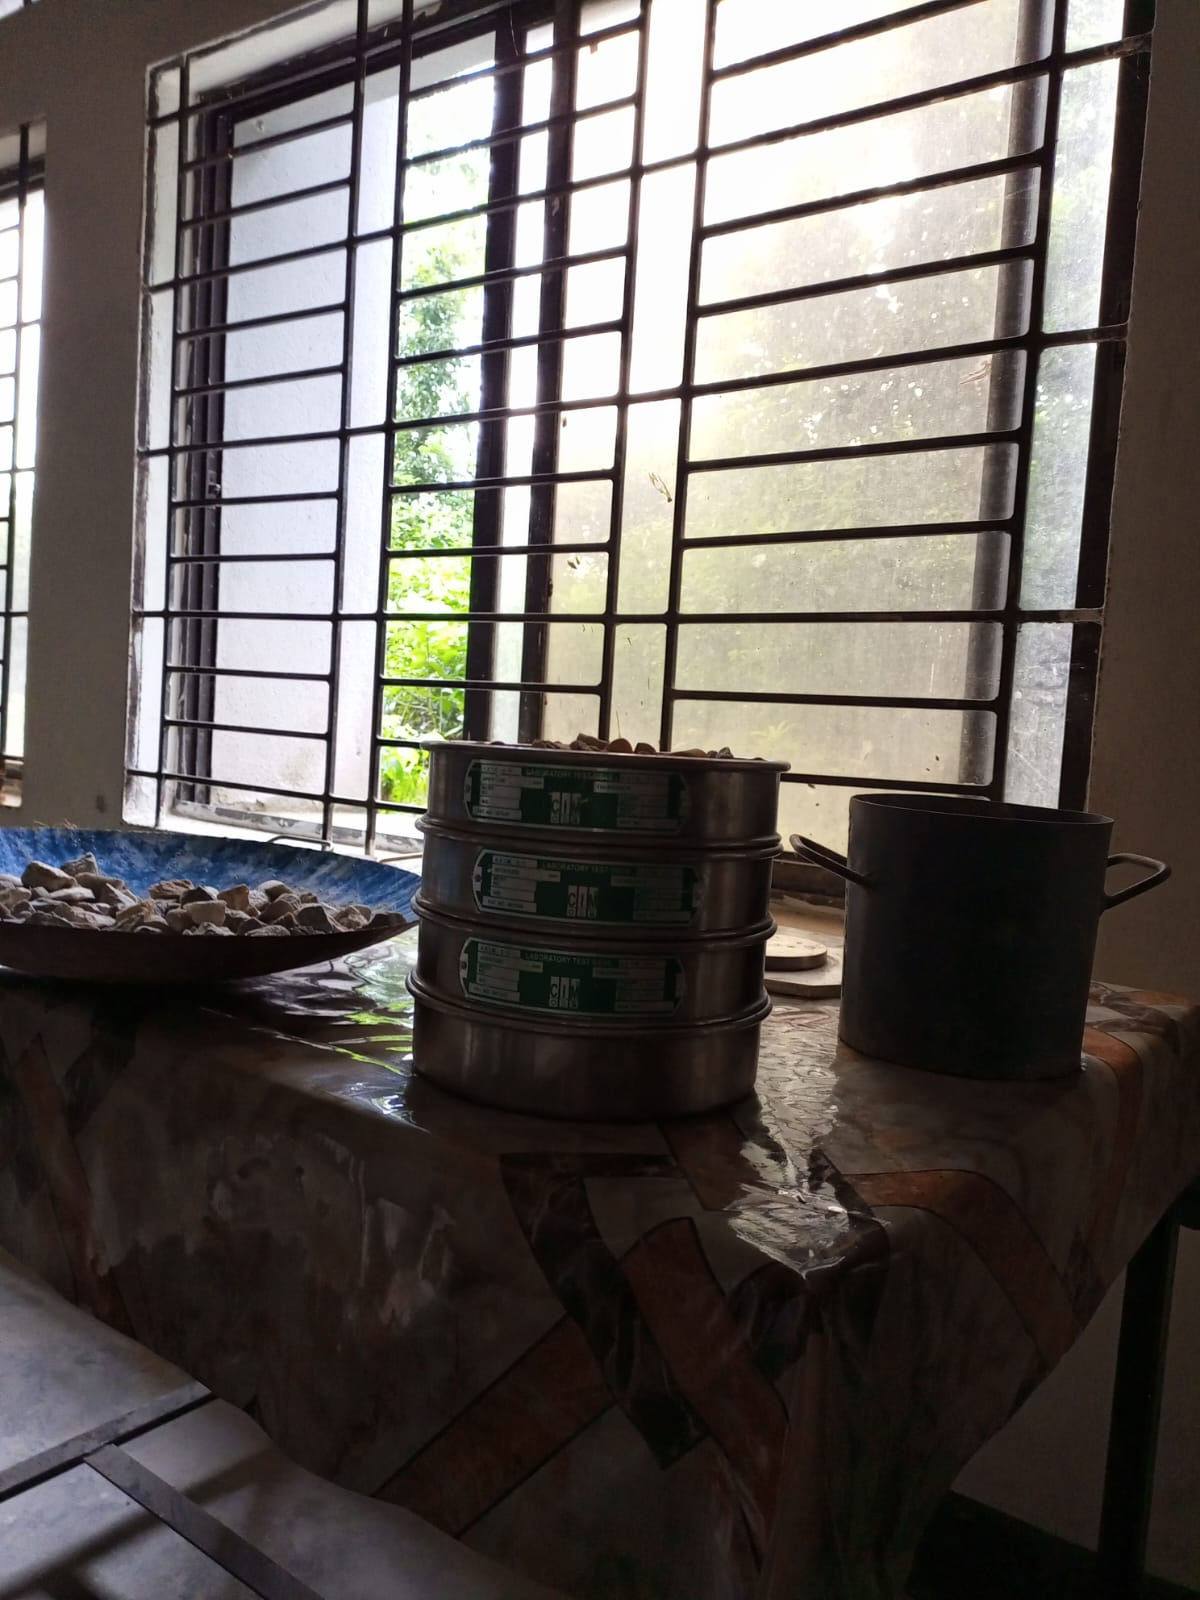
\includegraphics[width=4in, height=4in]{albums/appendix_21.jpeg}
\vspace{0.5cm}

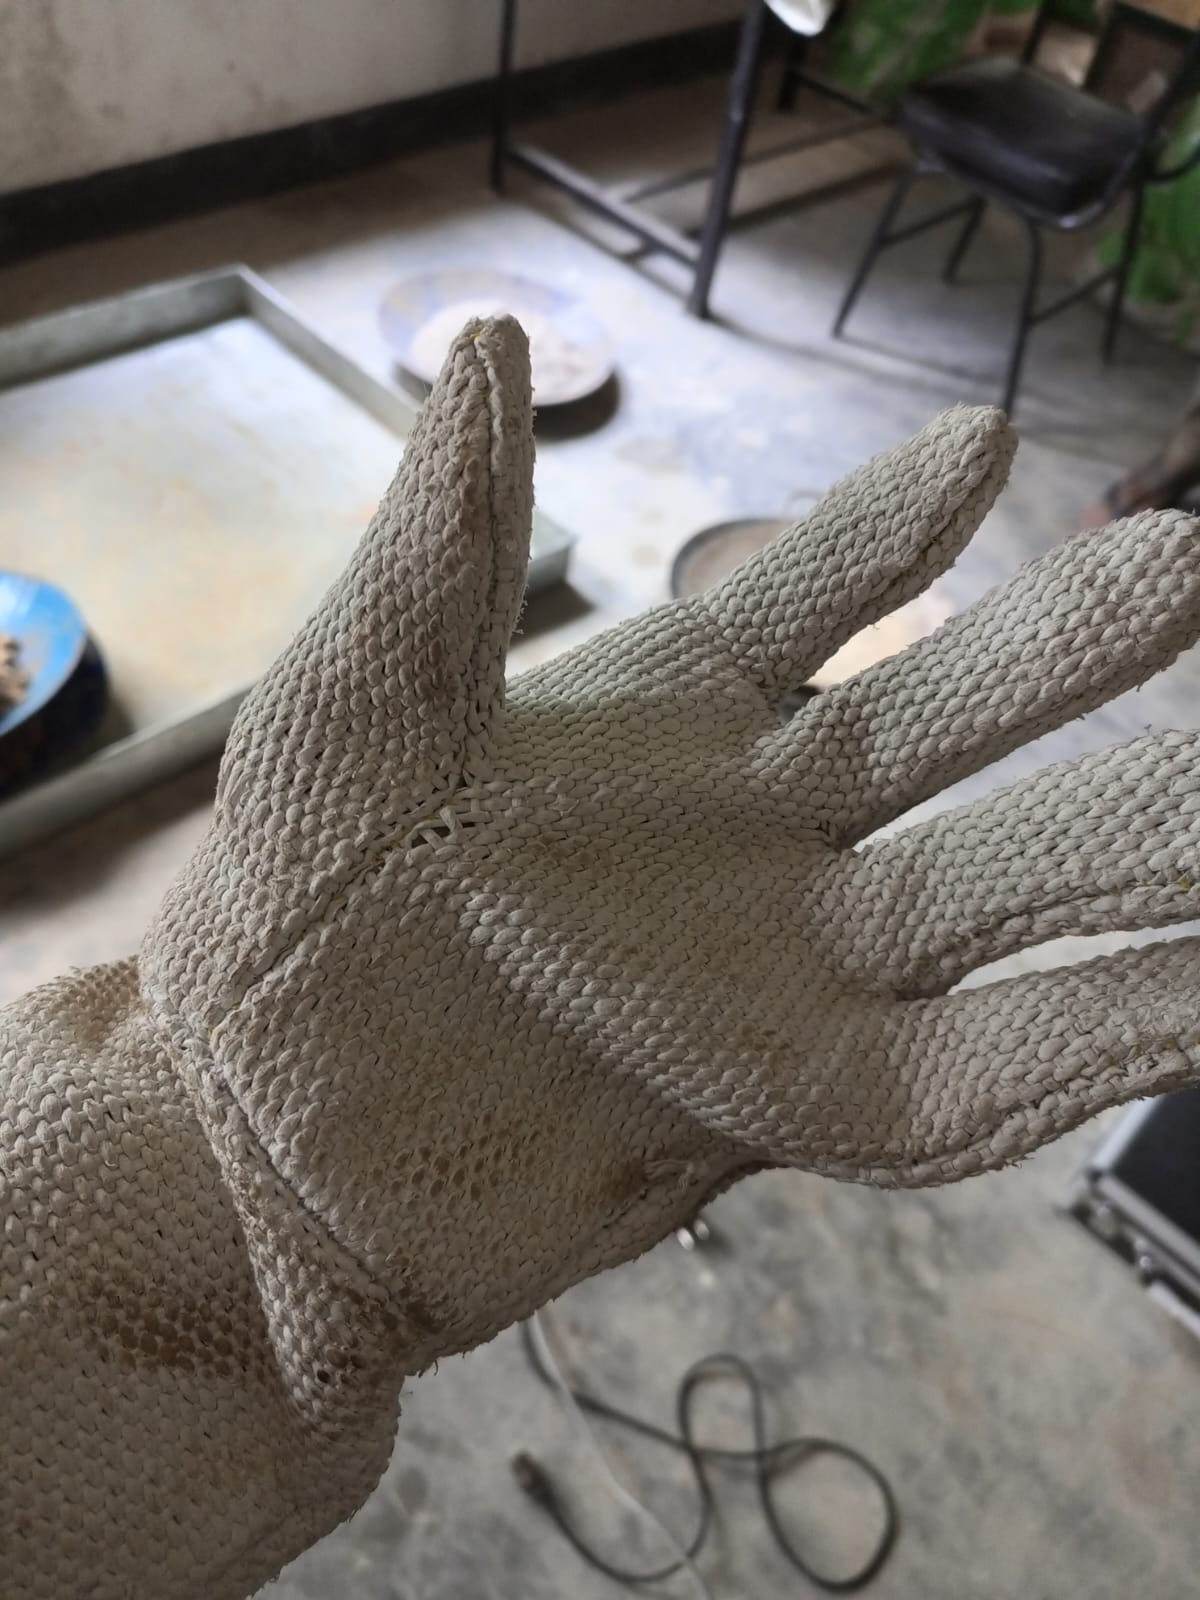
\includegraphics[width=4in, height=4in]{albums/appendix_22.jpeg}
\vspace{0.5cm}

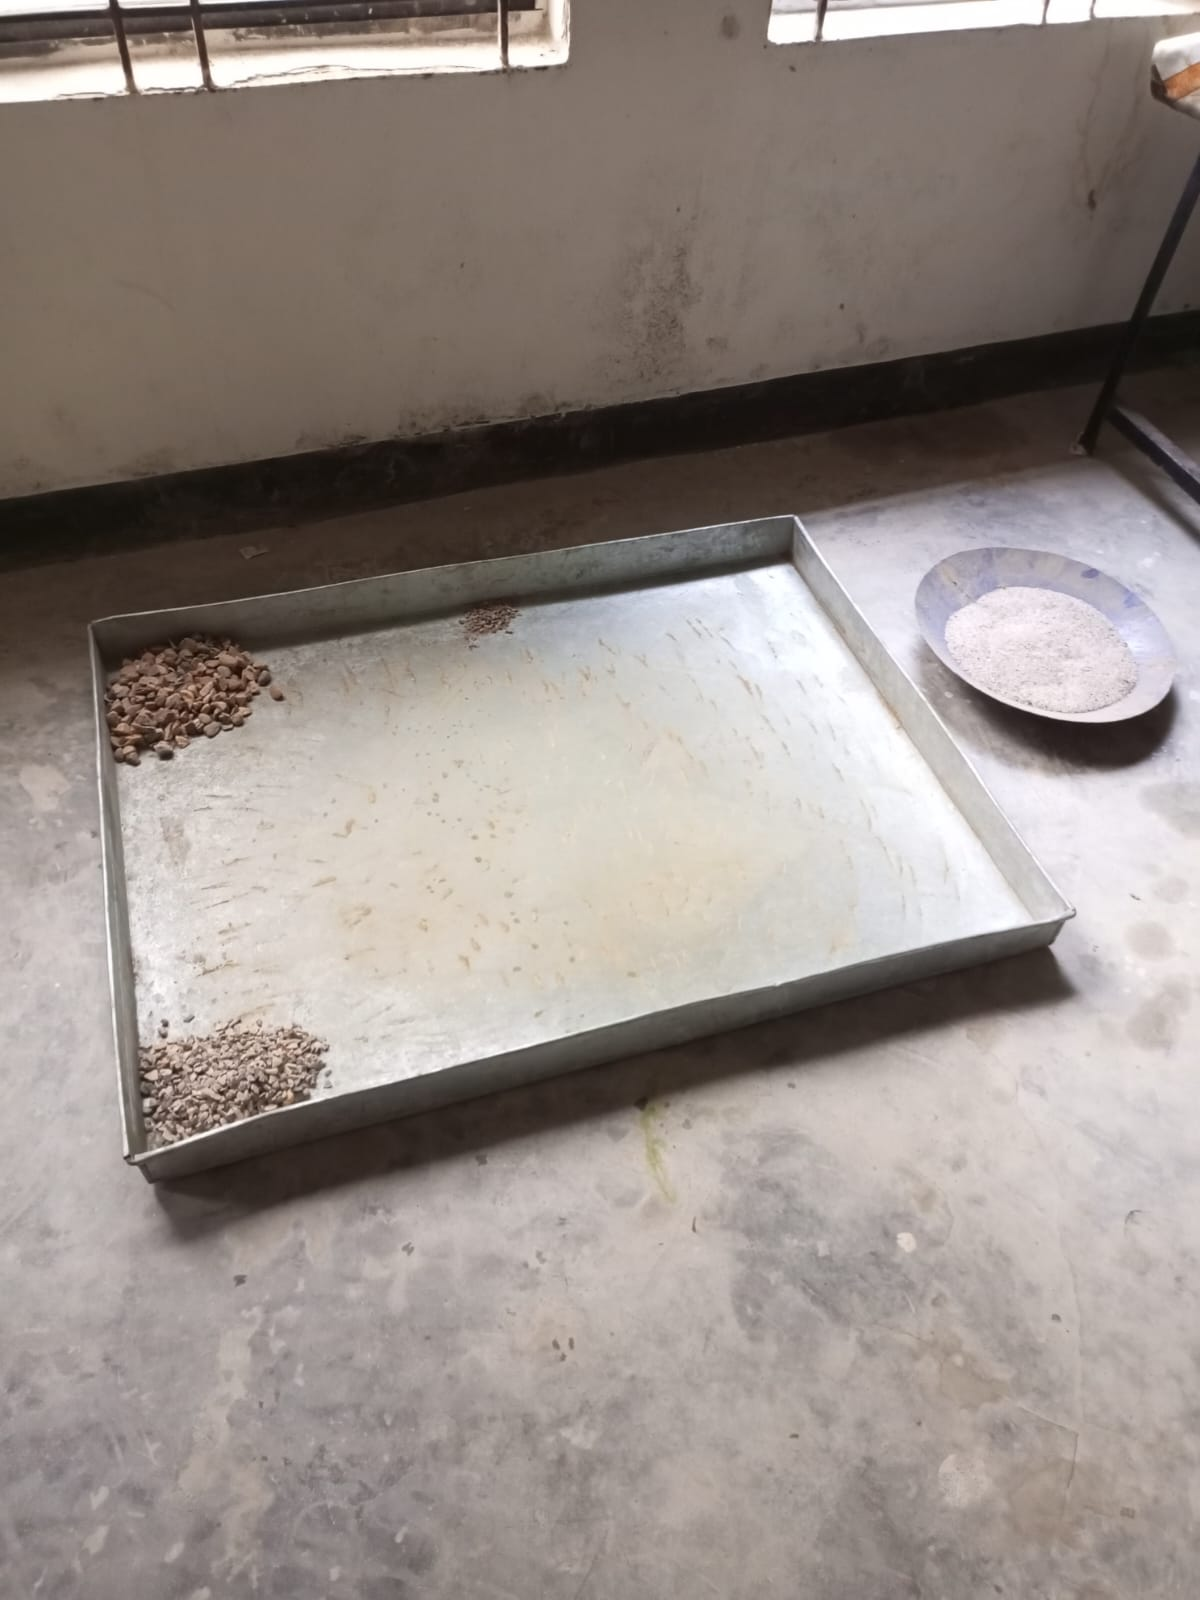
\includegraphics[width=4in, height=4in]{albums/appendix_23.jpeg}
\vspace{0.5cm}

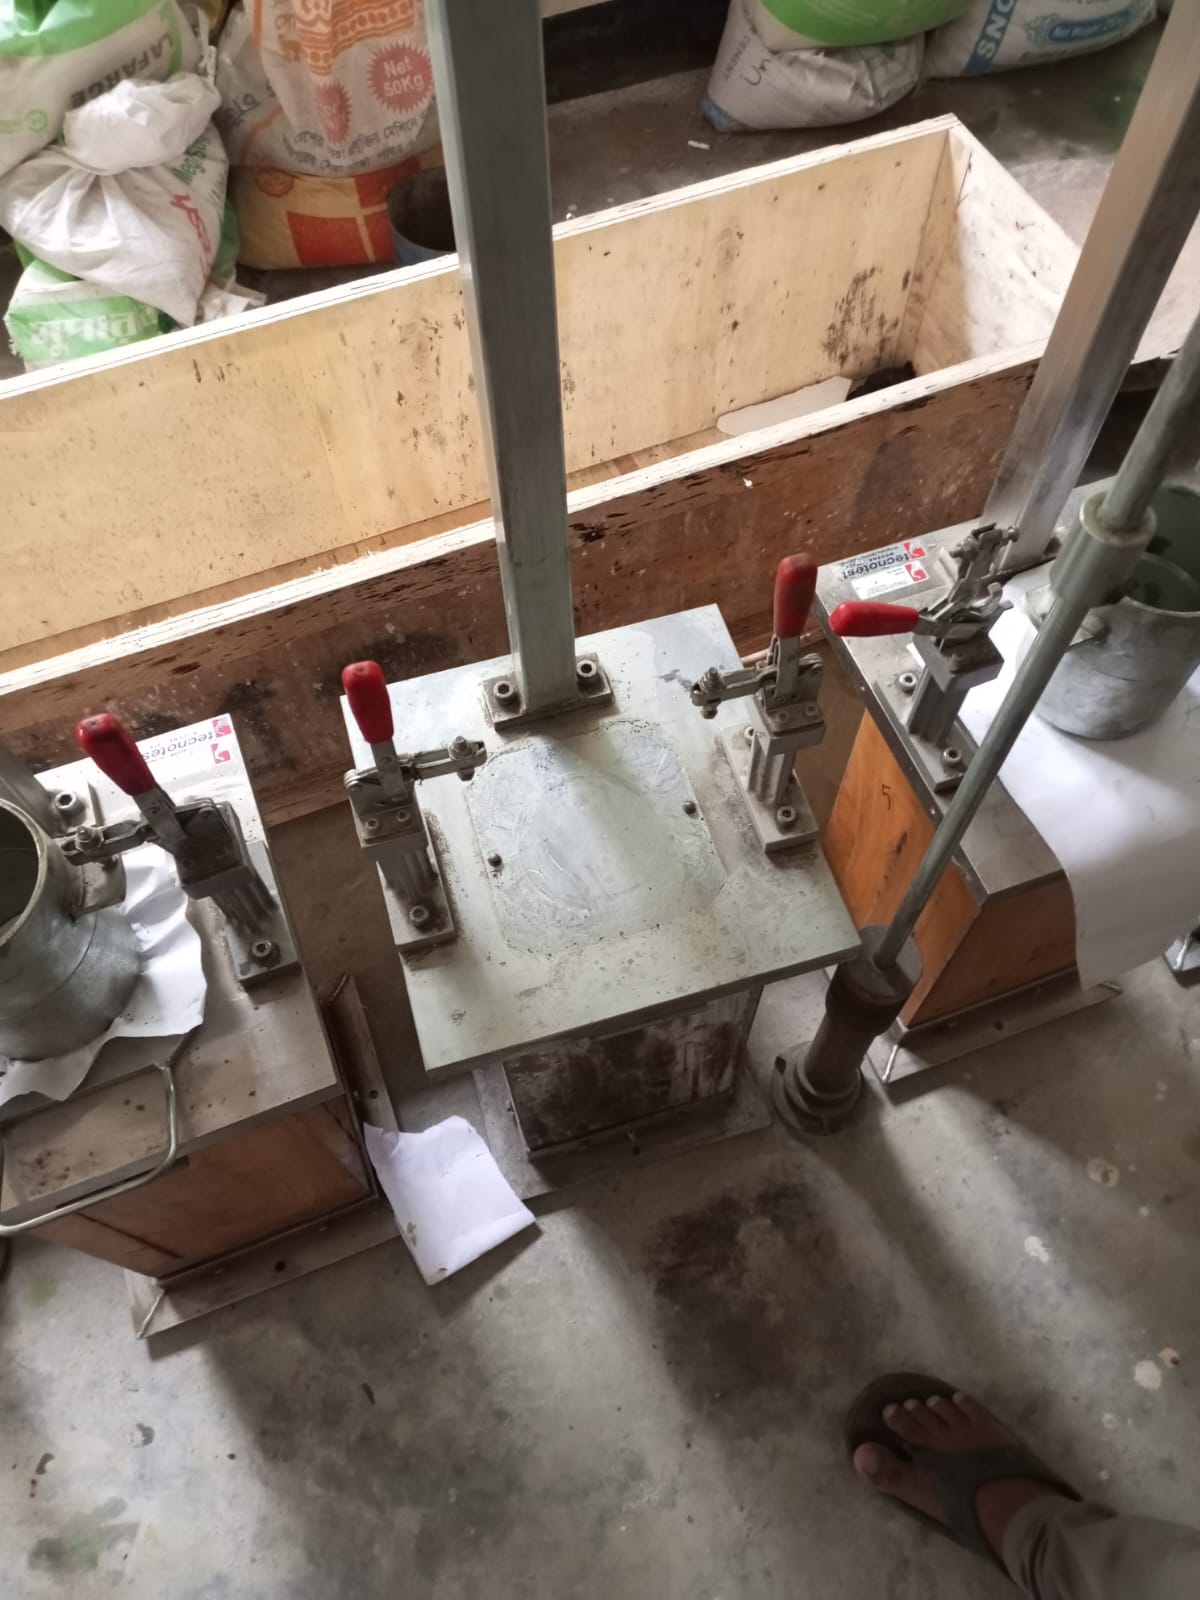
\includegraphics[width=4in, height=4in]{albums/appendix_24.jpeg}
\vspace{0.5cm}

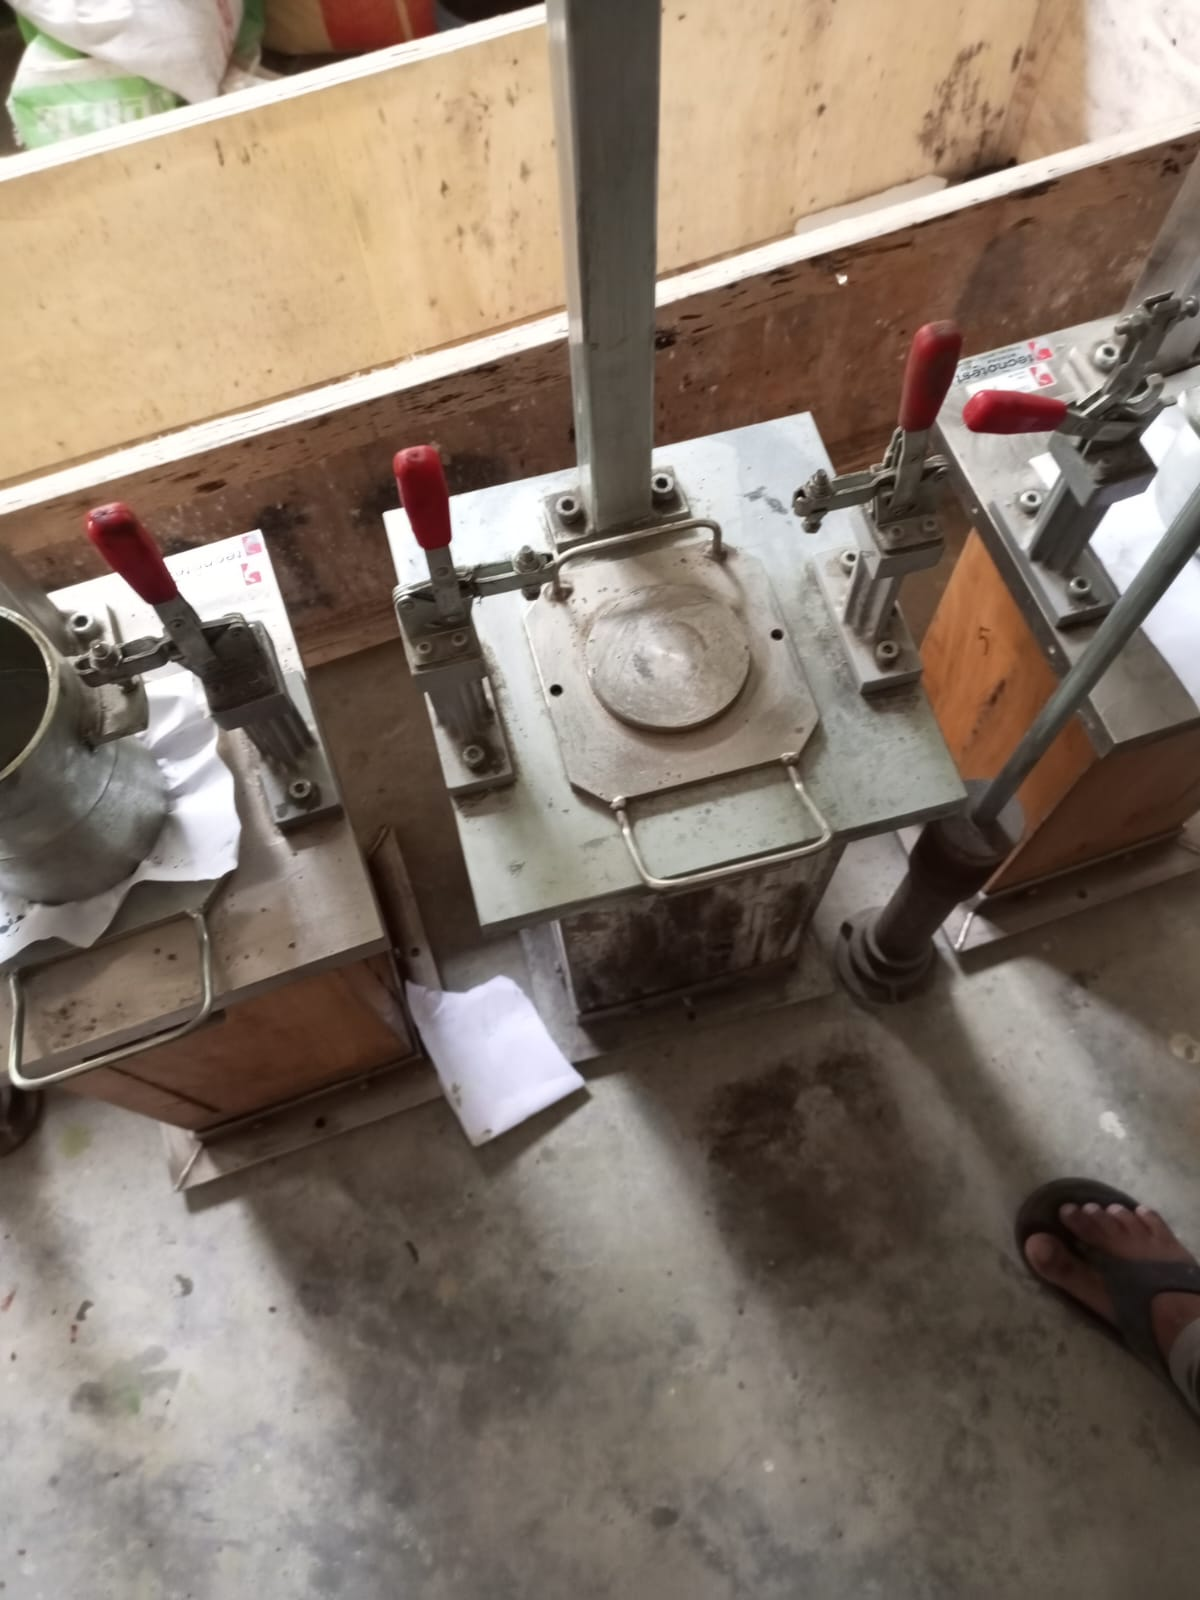
\includegraphics[width=4in, height=4in]{albums/appendix_25.jpeg}
\vspace{0.5cm}

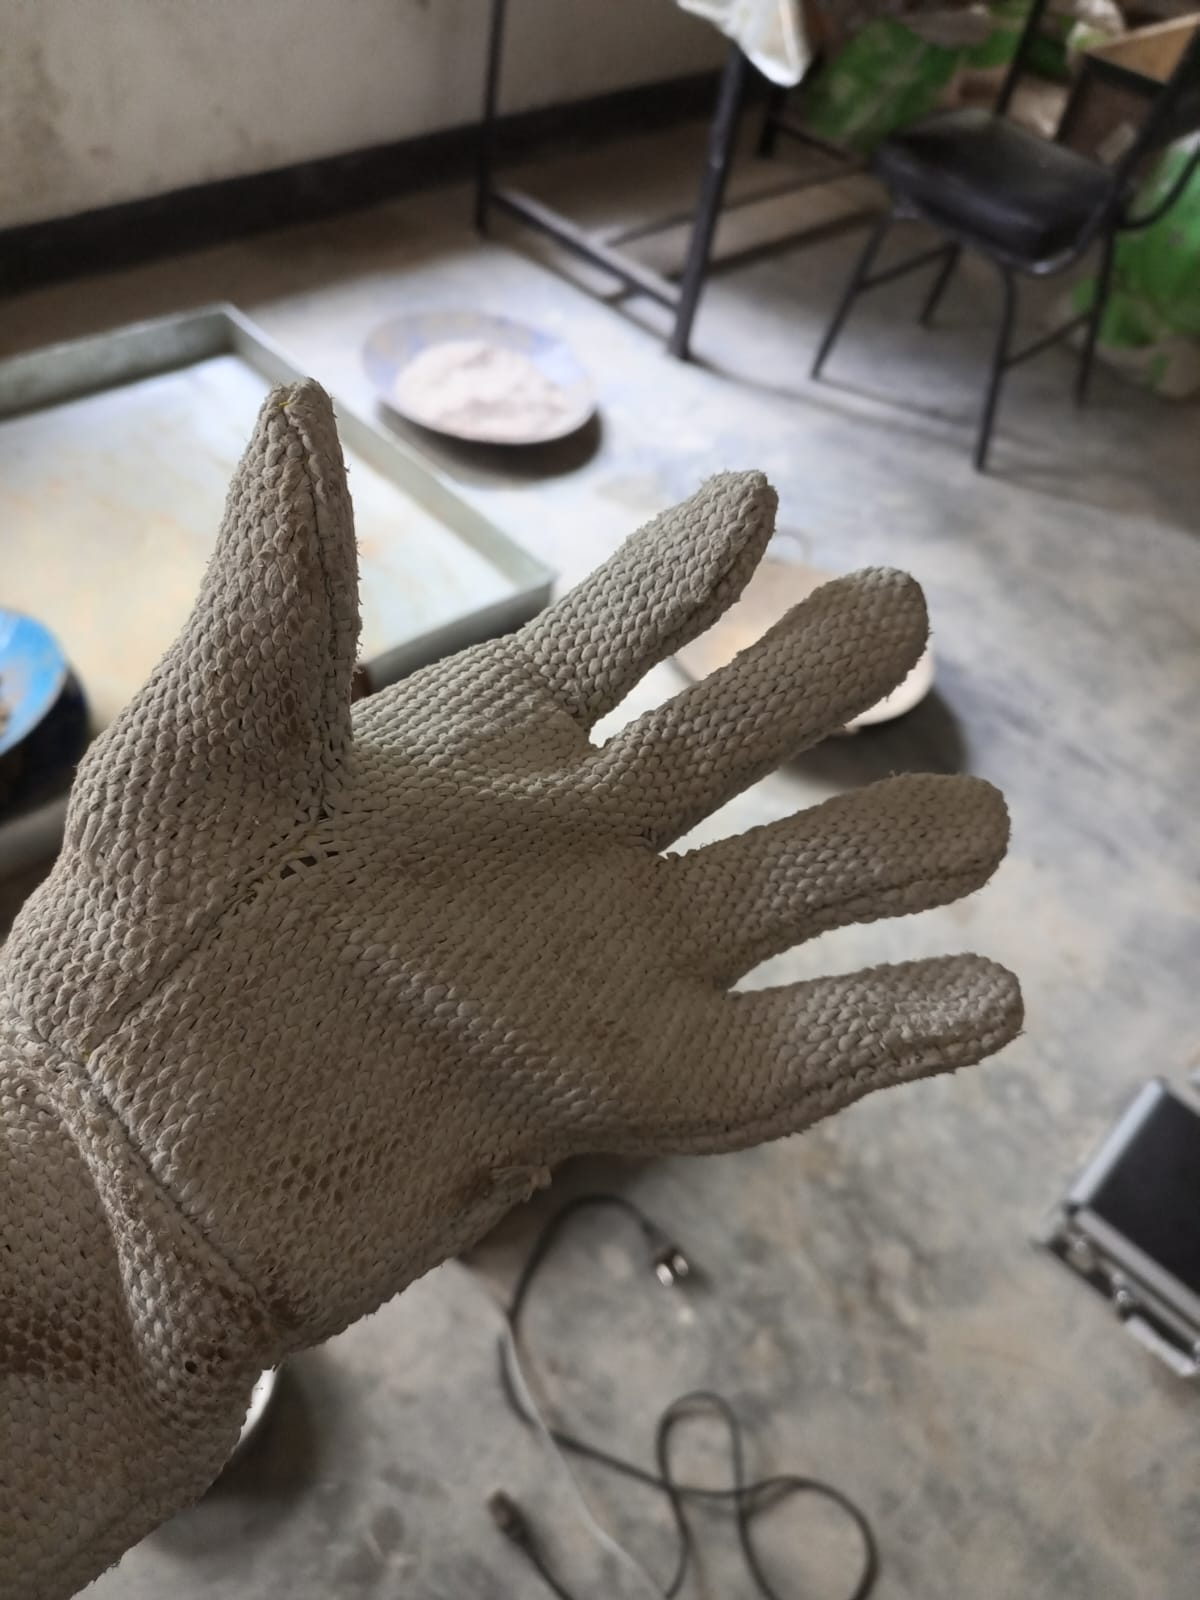
\includegraphics[width=4in, height=4in]{albums/appendix_26.jpeg}
\vspace{0.5cm}

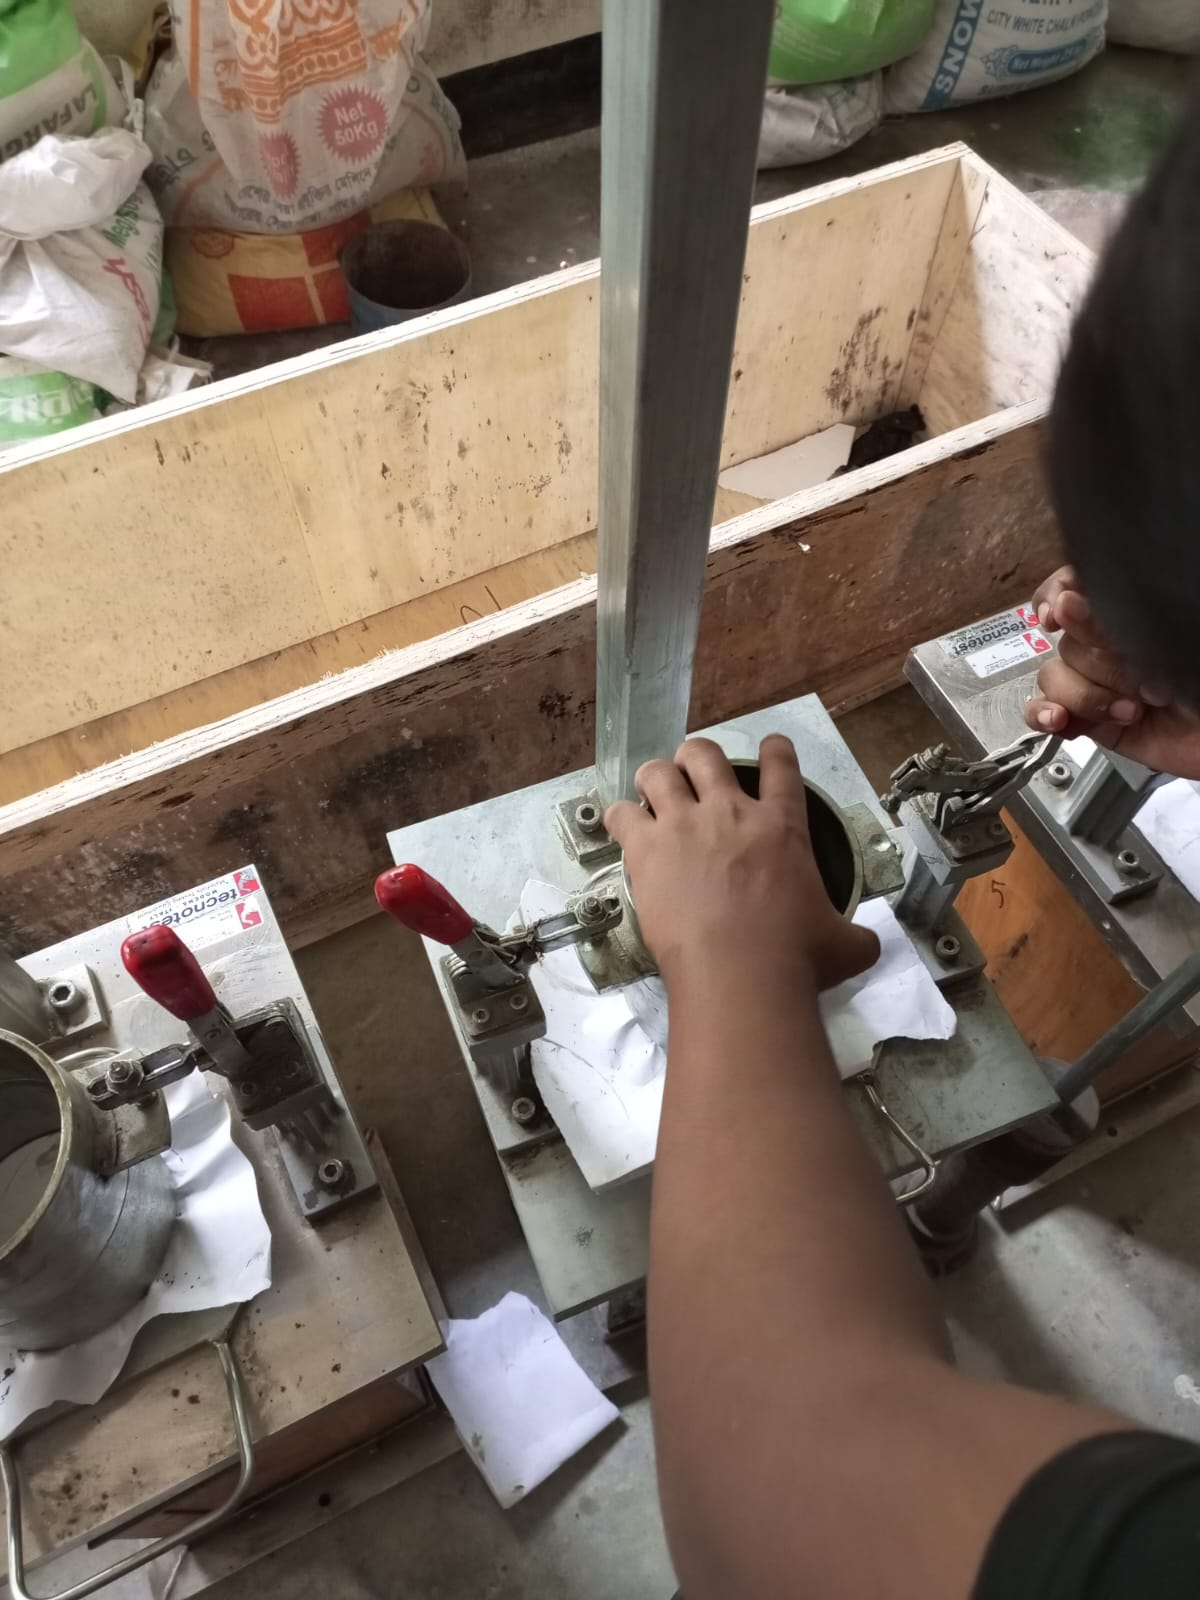
\includegraphics[width=4in, height=4in]{albums/appendix_27.jpeg}
\vspace{0.5cm}

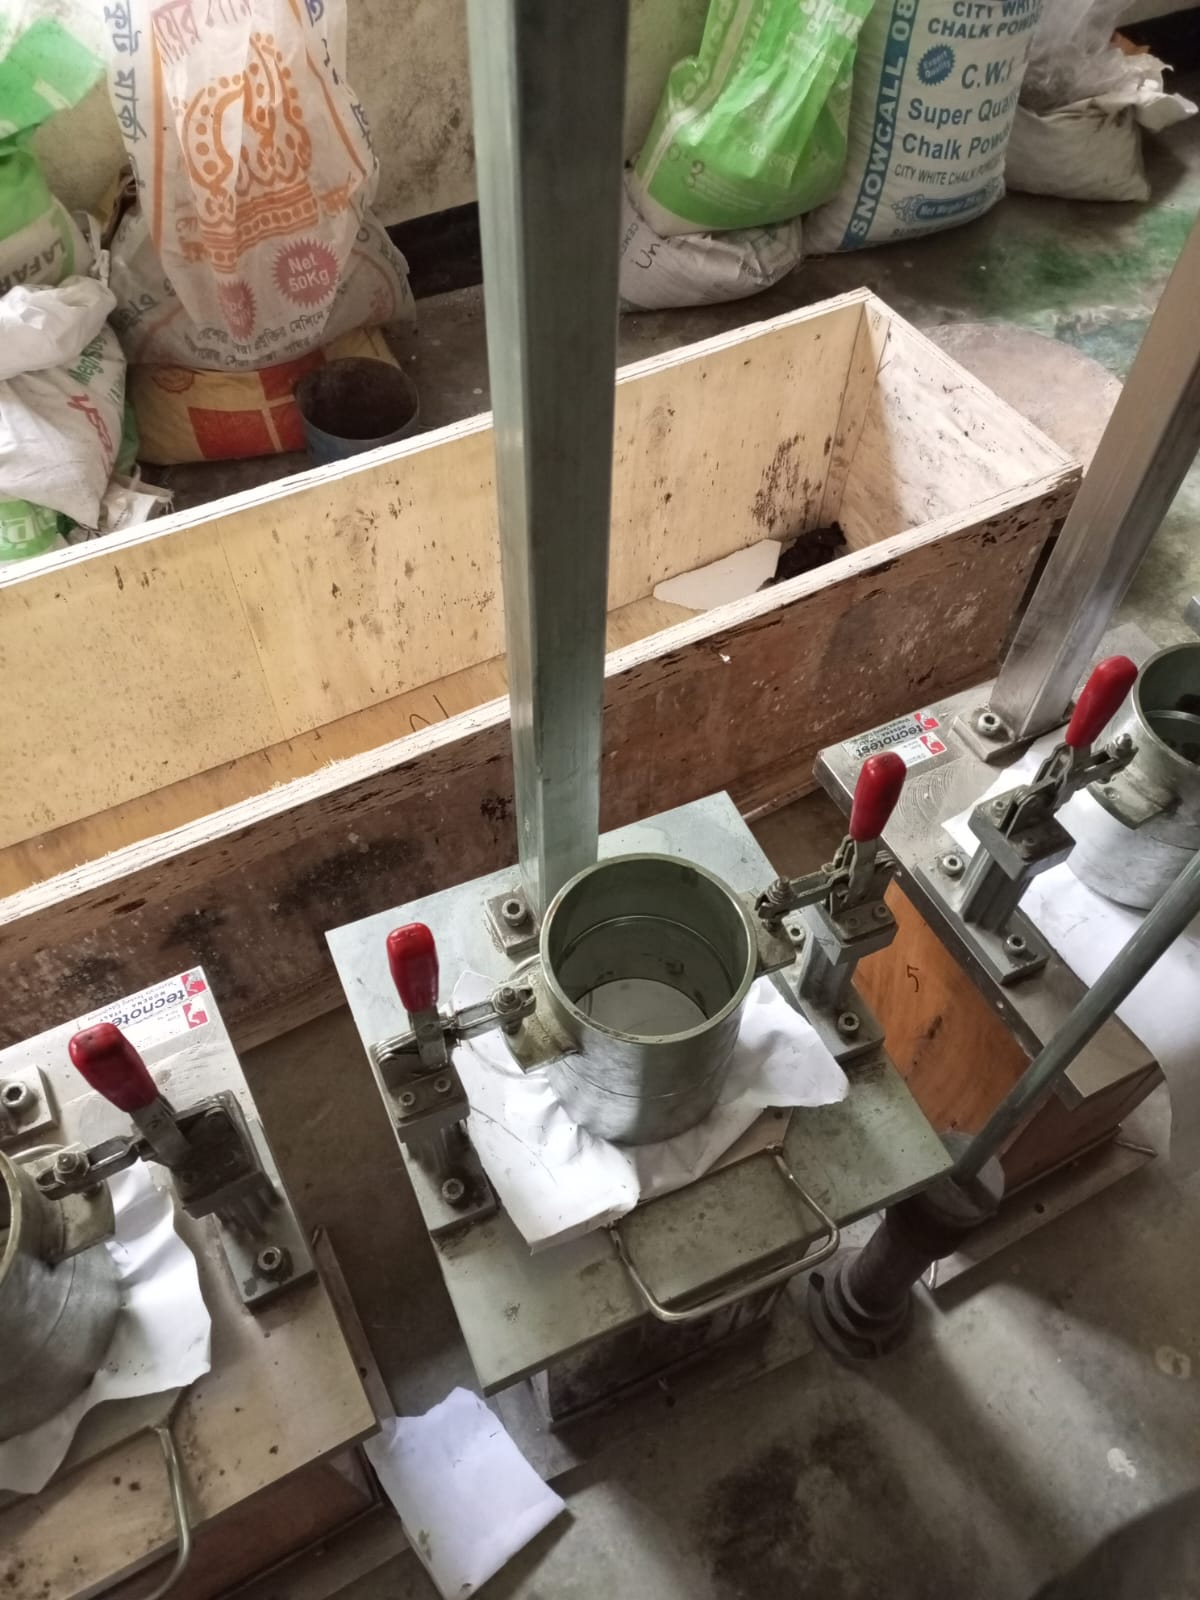
\includegraphics[width=4in, height=4in]{albums/appendix_28.jpeg}
\vspace{0.5cm}

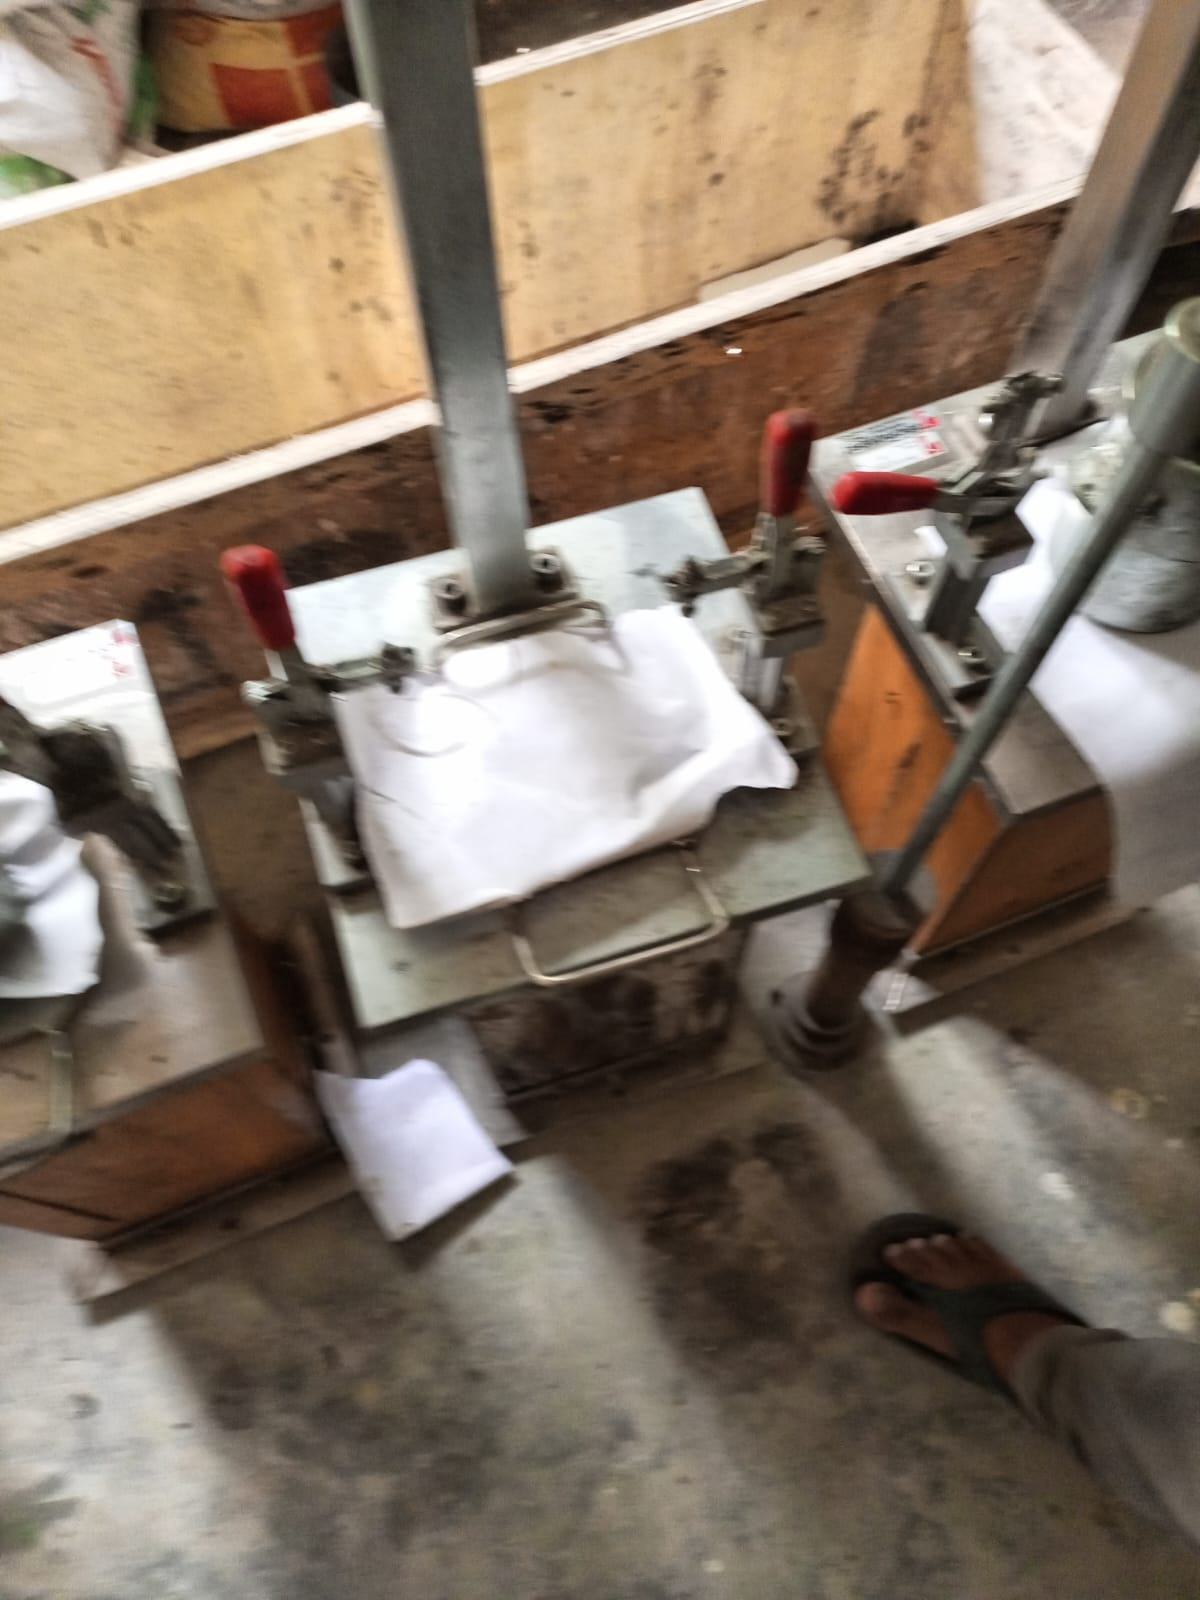
\includegraphics[width=4in, height=4in]{albums/appendix_29.jpeg}
\vspace{0.5cm}

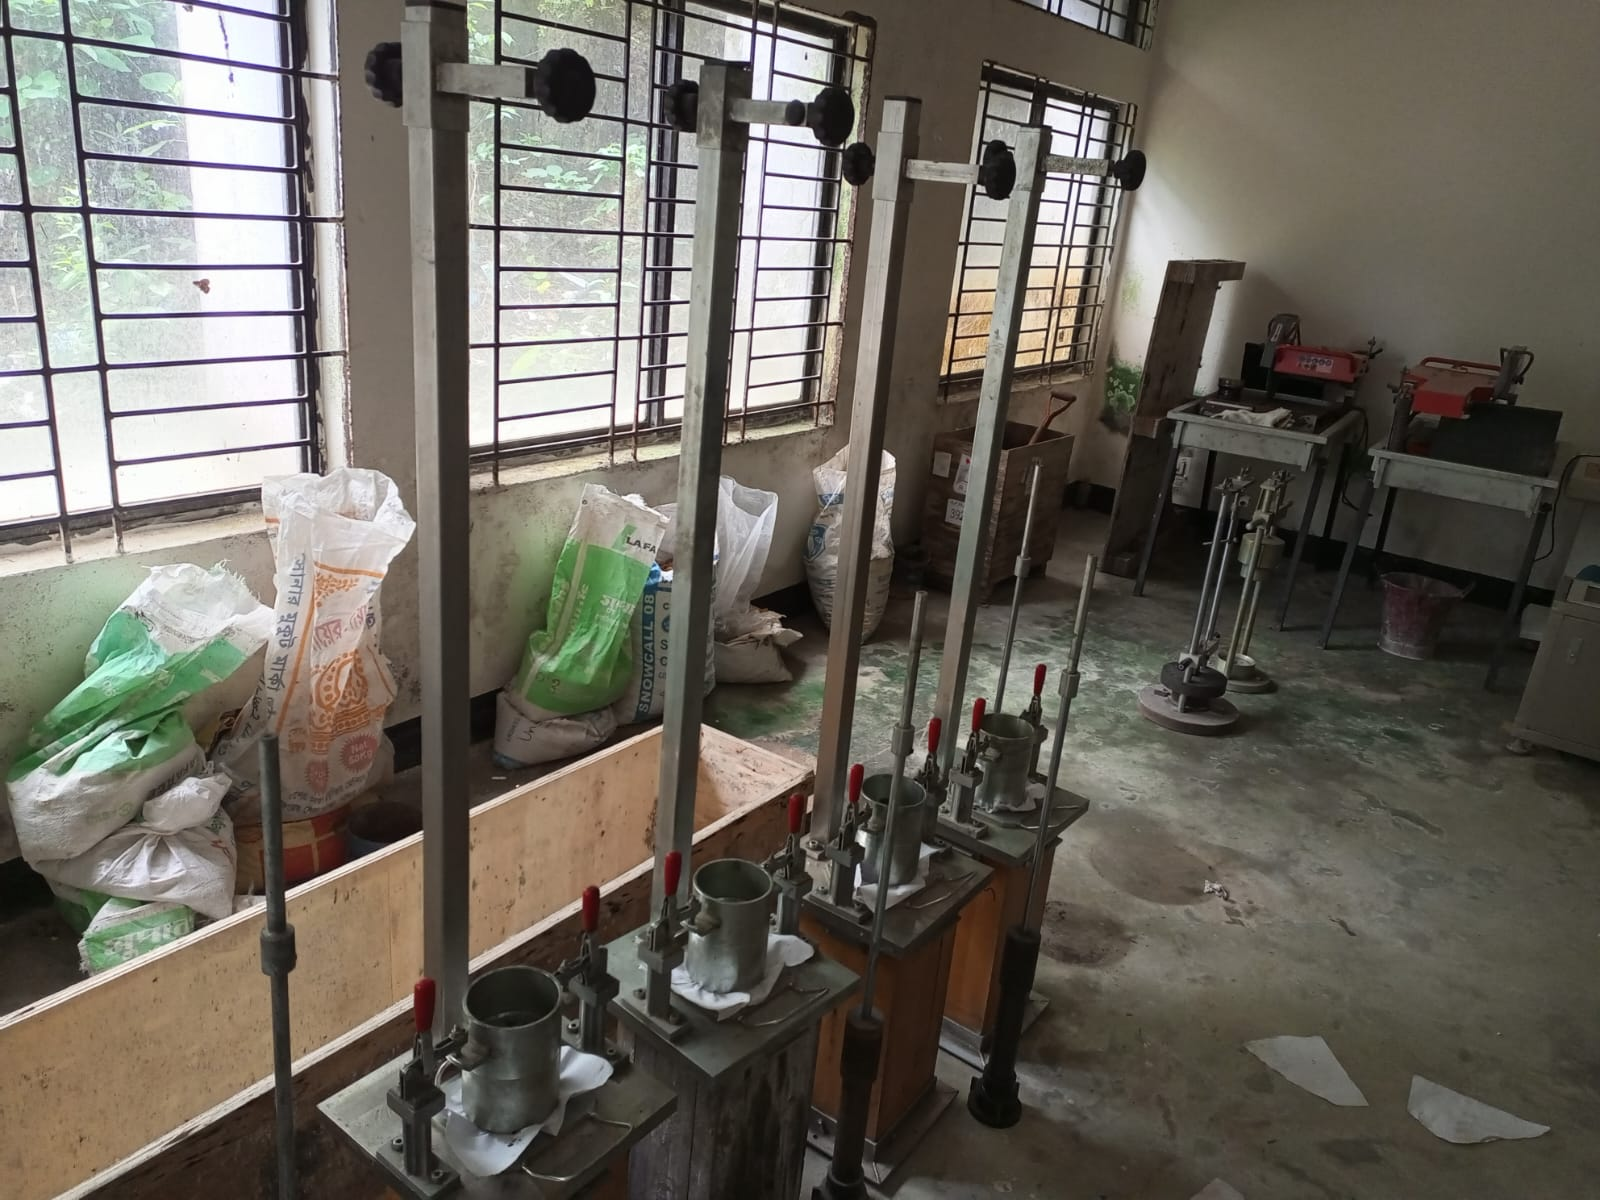
\includegraphics[width=4in, height=4in]{albums/appendix_30.jpeg}
\vspace{0.5cm}

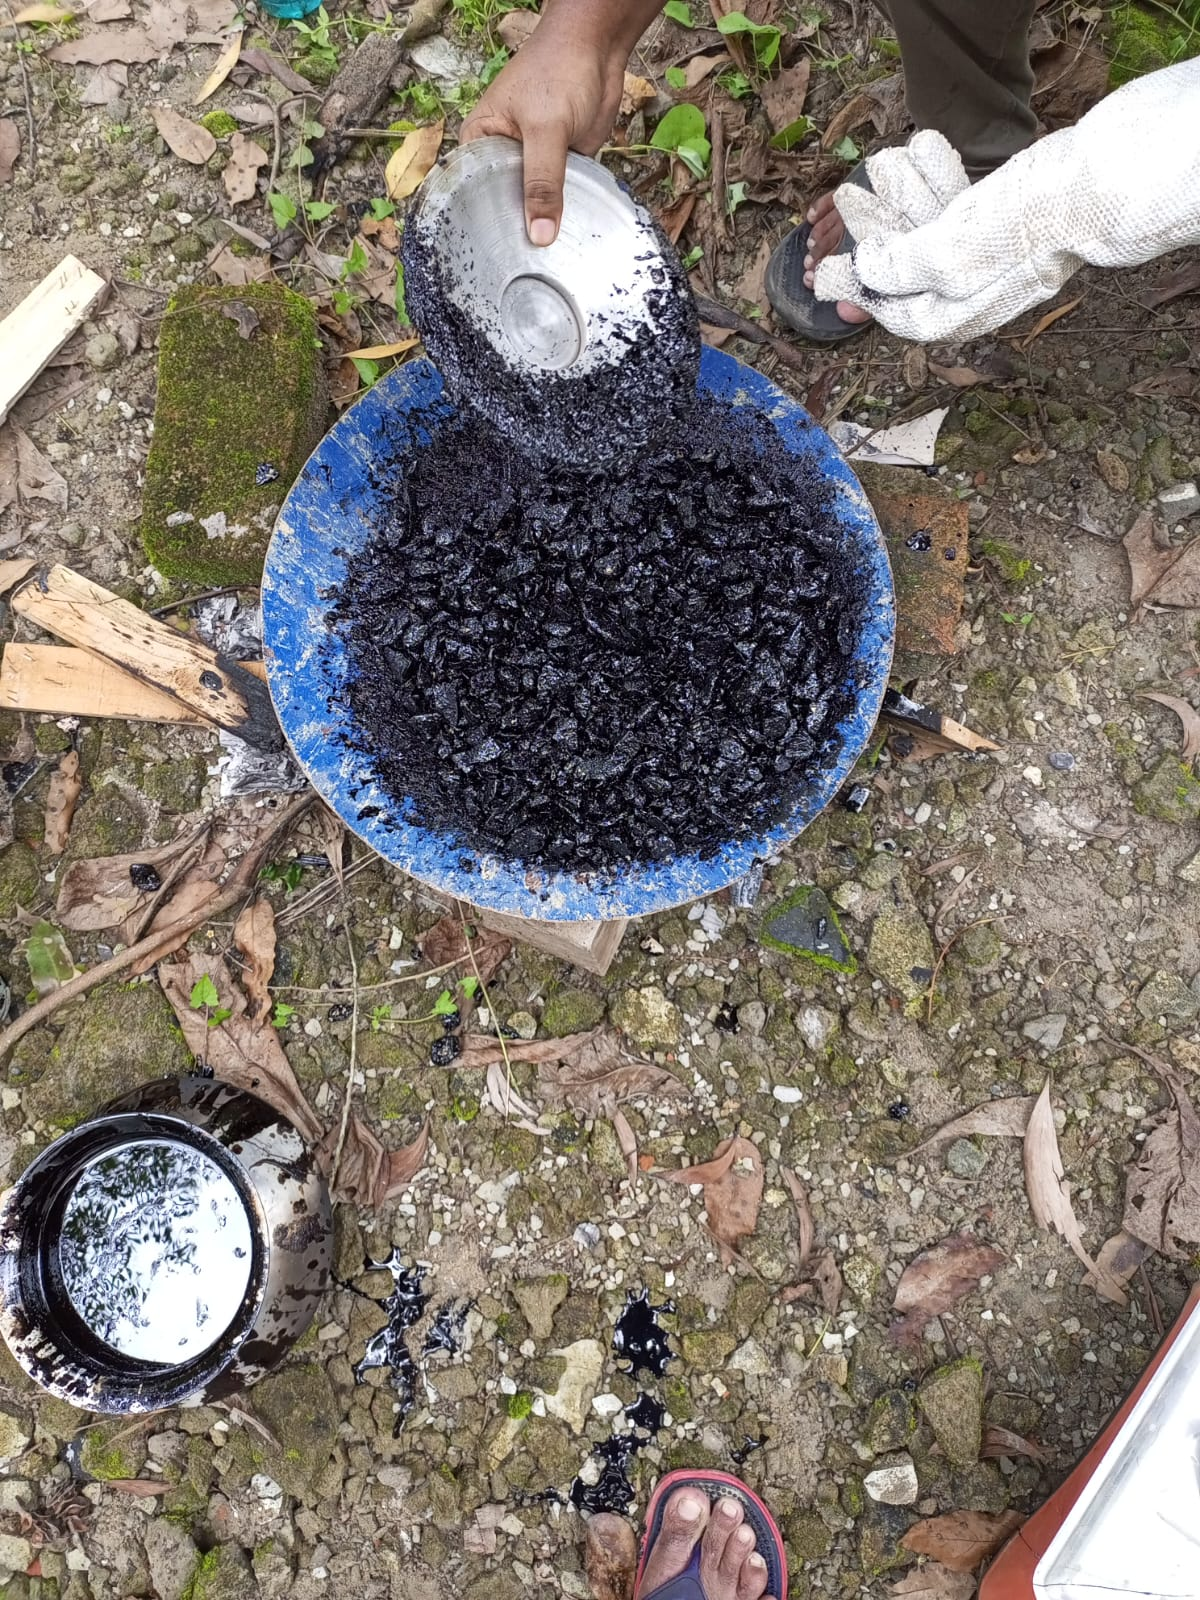
\includegraphics[width=4in, height=4in]{albums/appendix_31.jpeg}
\vspace{0.5cm}

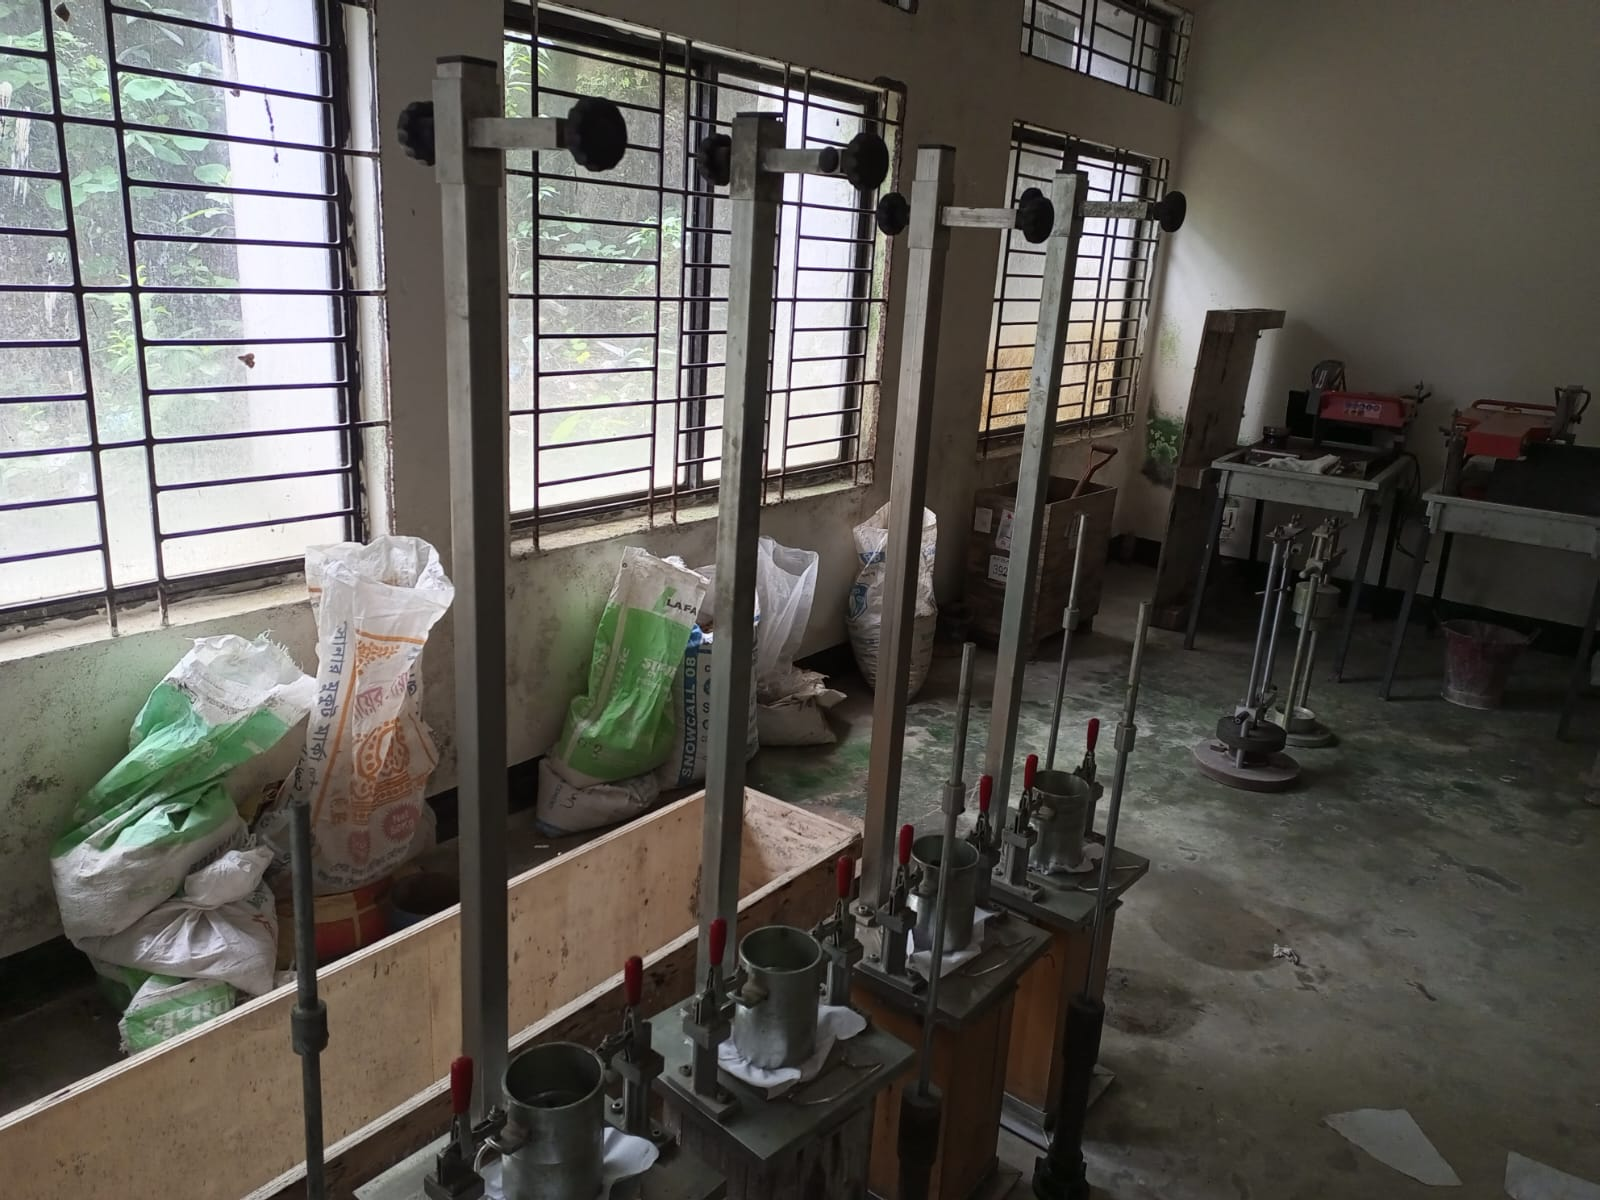
\includegraphics[width=4in, height=4in]{albums/appendix_32.jpeg}
\vspace{0.5cm}

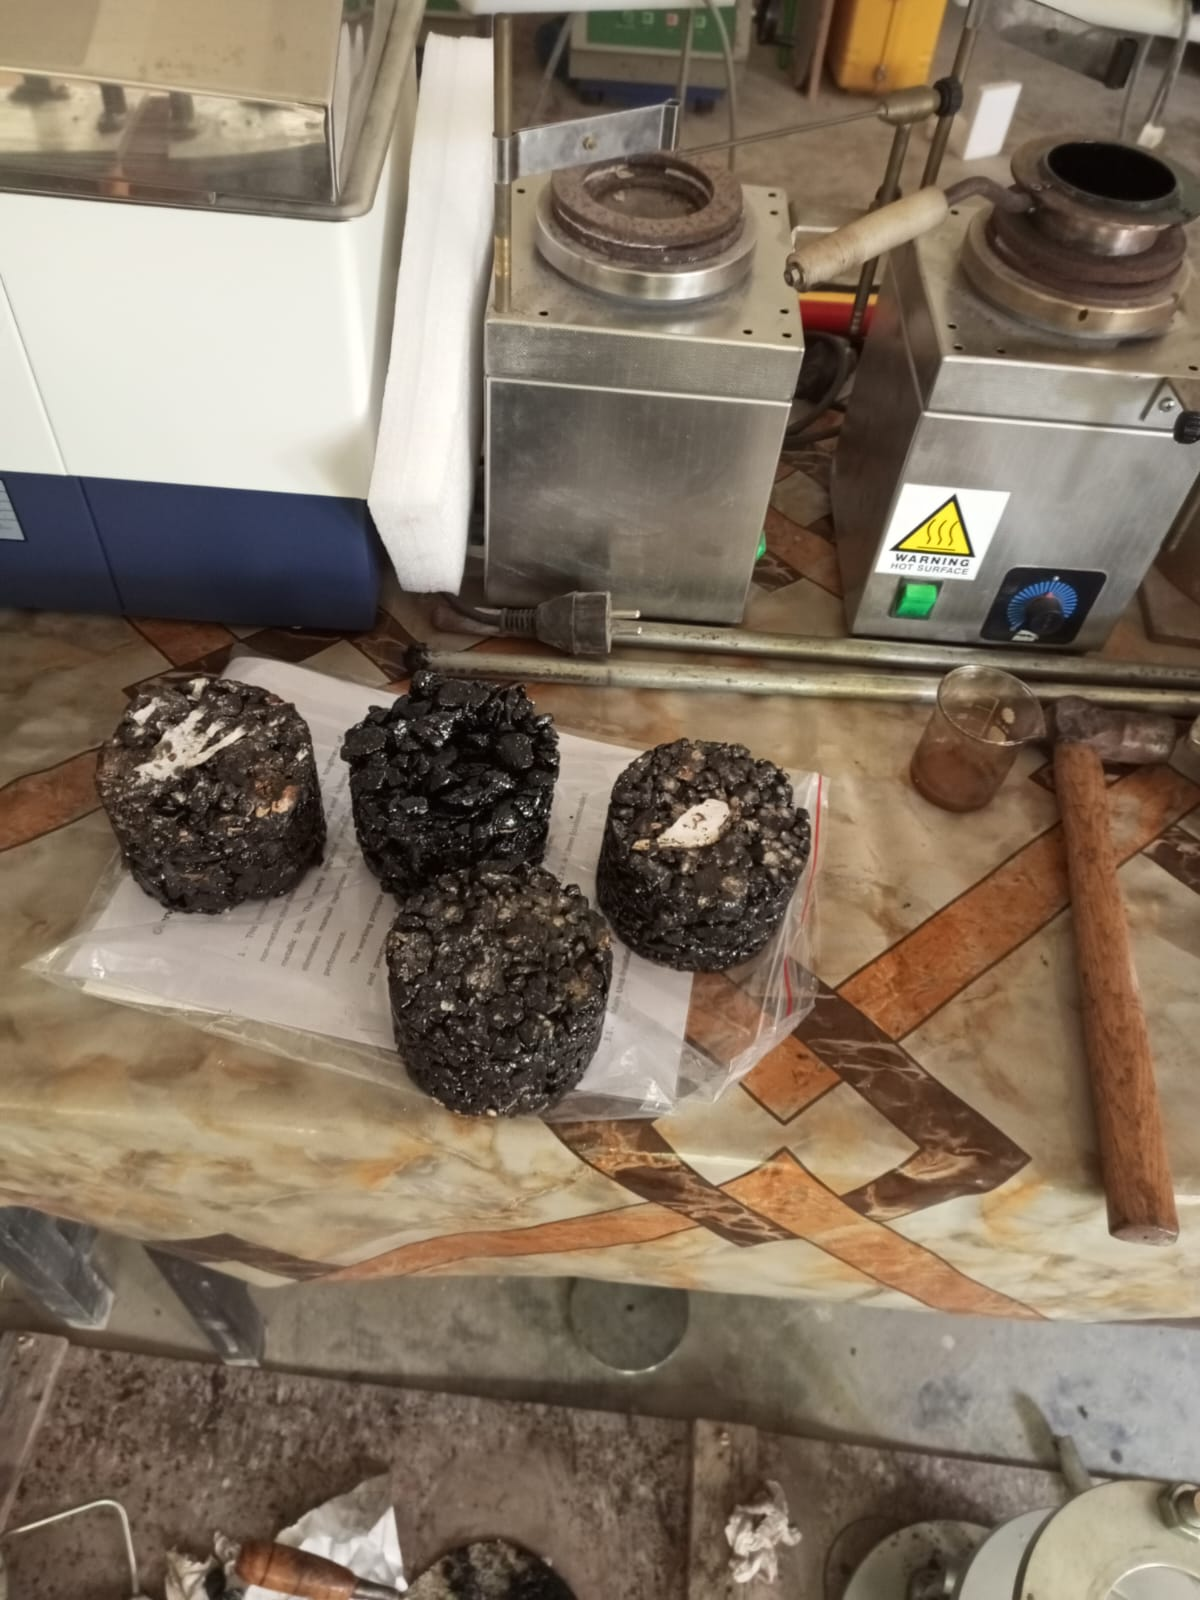
\includegraphics[width=4in, height=4in]{albums/appendix_33.jpeg}
\vspace{0.5cm}

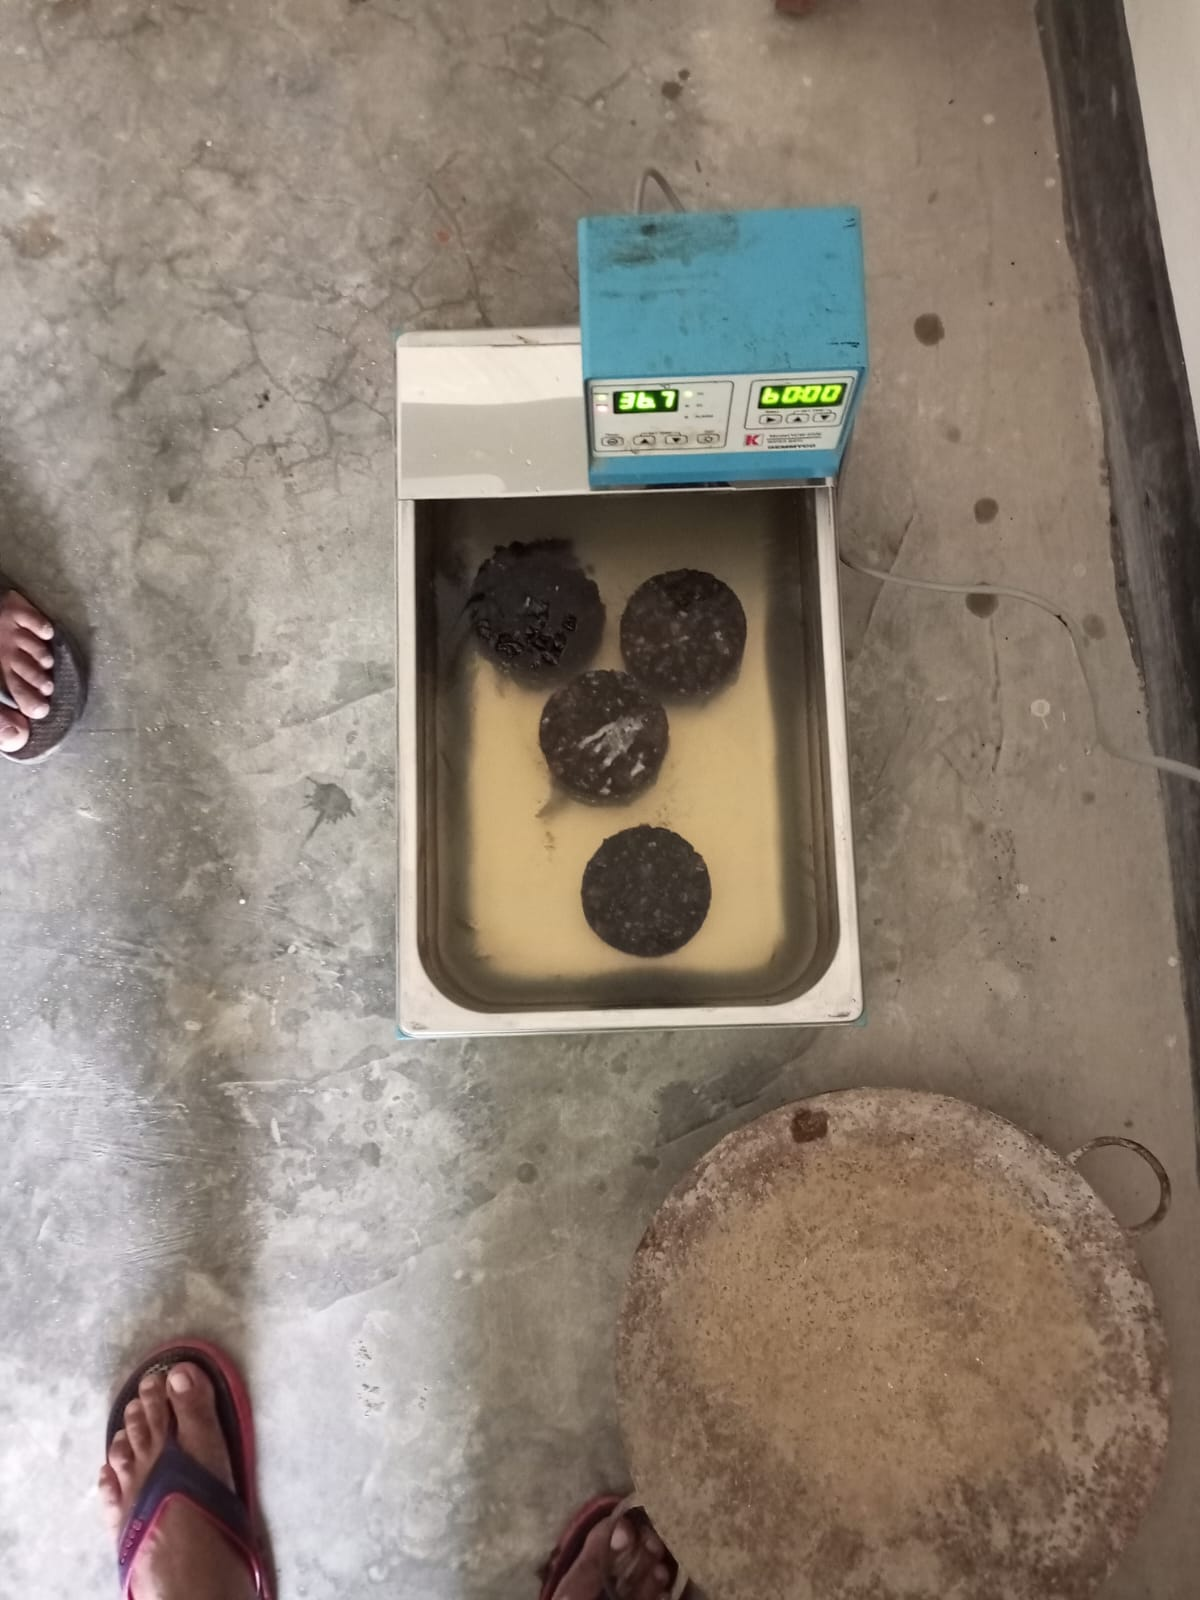
\includegraphics[width=4in, height=4in]{albums/appendix_34.jpeg}
\vspace{0.5cm}

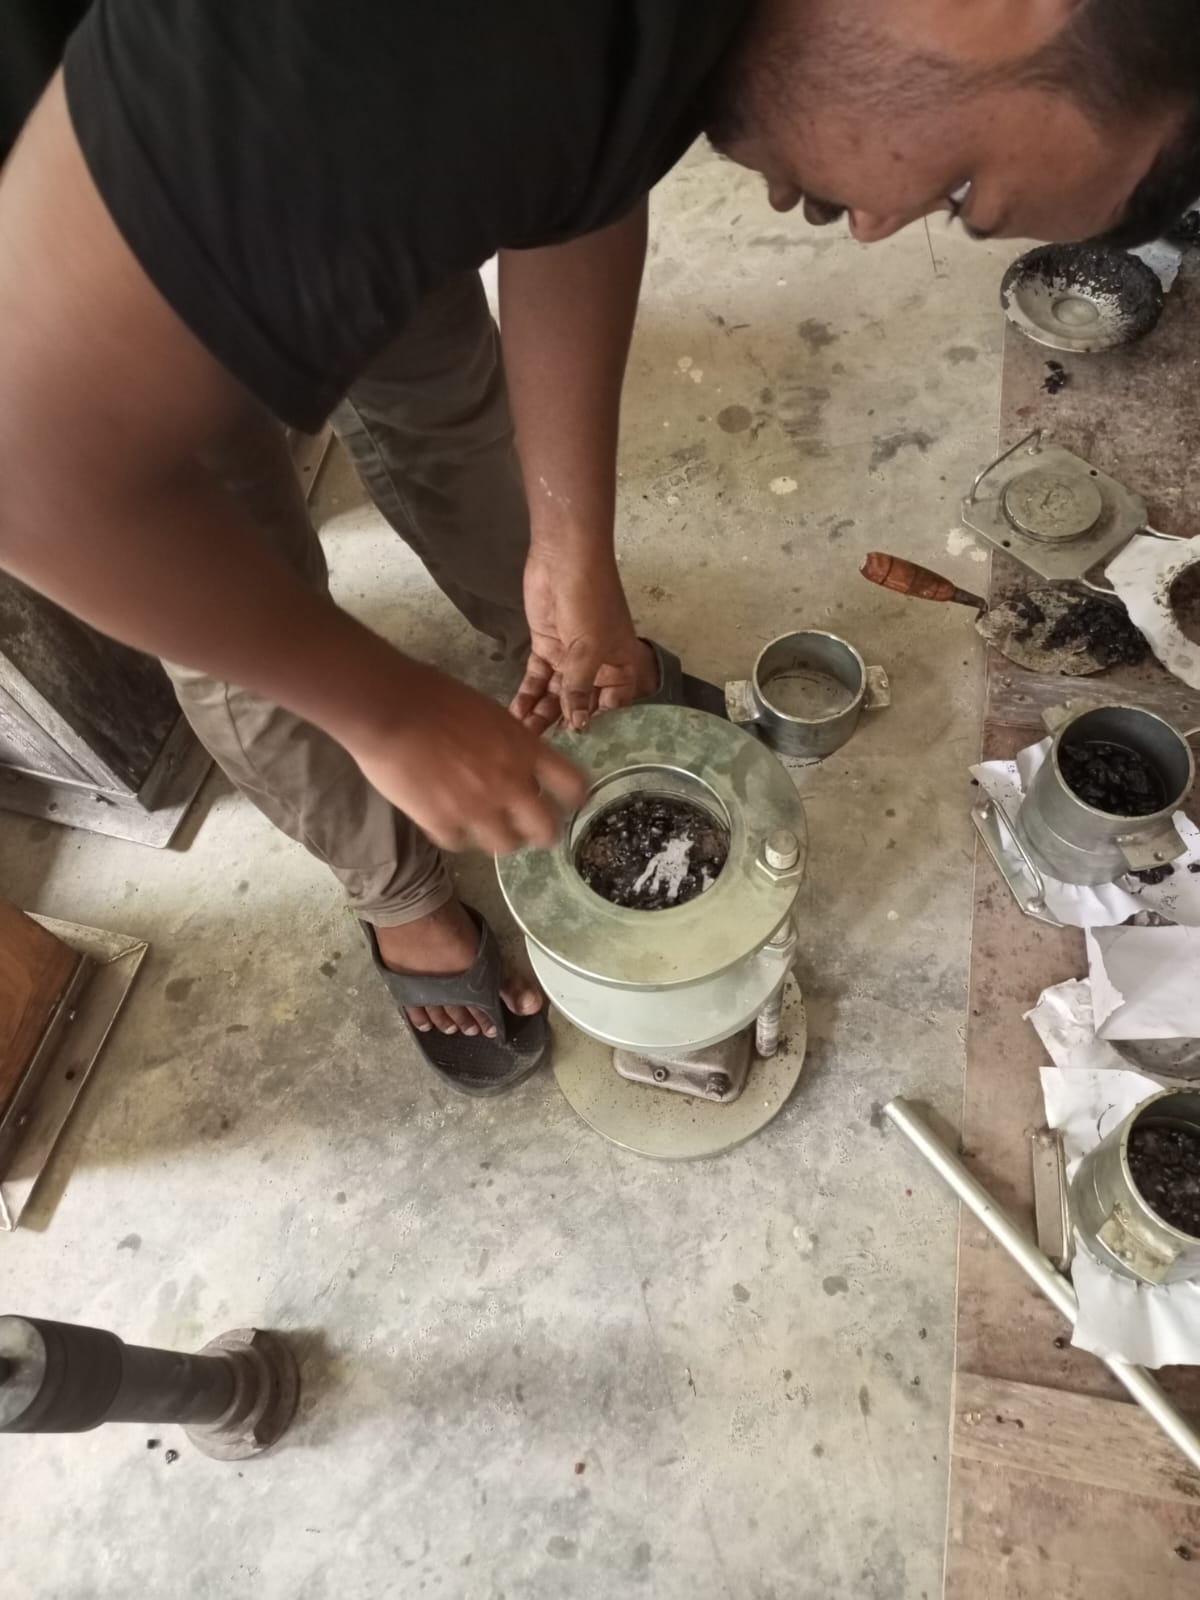
\includegraphics[width=4in, height=4in]{albums/appendix_35.jpeg}
\vspace{0.5cm}

\end{center}

\end{document}